\subsection{Déroulé de la semaine}

\subsubsection{Préparation et contrôles initiaux}
L'équipe est arrivée au C'Space avec une fusée entièrement peinte et un premier étage intégré, prêt à recevoir 
le deuxième. Cependant, l'intégration électrique de ce dernier n'était pas finalisée en raison 
d'un changement de position de deux PCB en lien avec la dernière position des batteries, nécessaire pour ajuster 
le centre de masse comme convenu dans le Stabtraj. Ce contretemps, parmi d'autres, a causé quelques retards pour tout
passage en contrôle dès dimanche après-midi.

\begin{figure}[!ht]
    \centering
    \begin{subfigure}[b]{0.63\textwidth}
        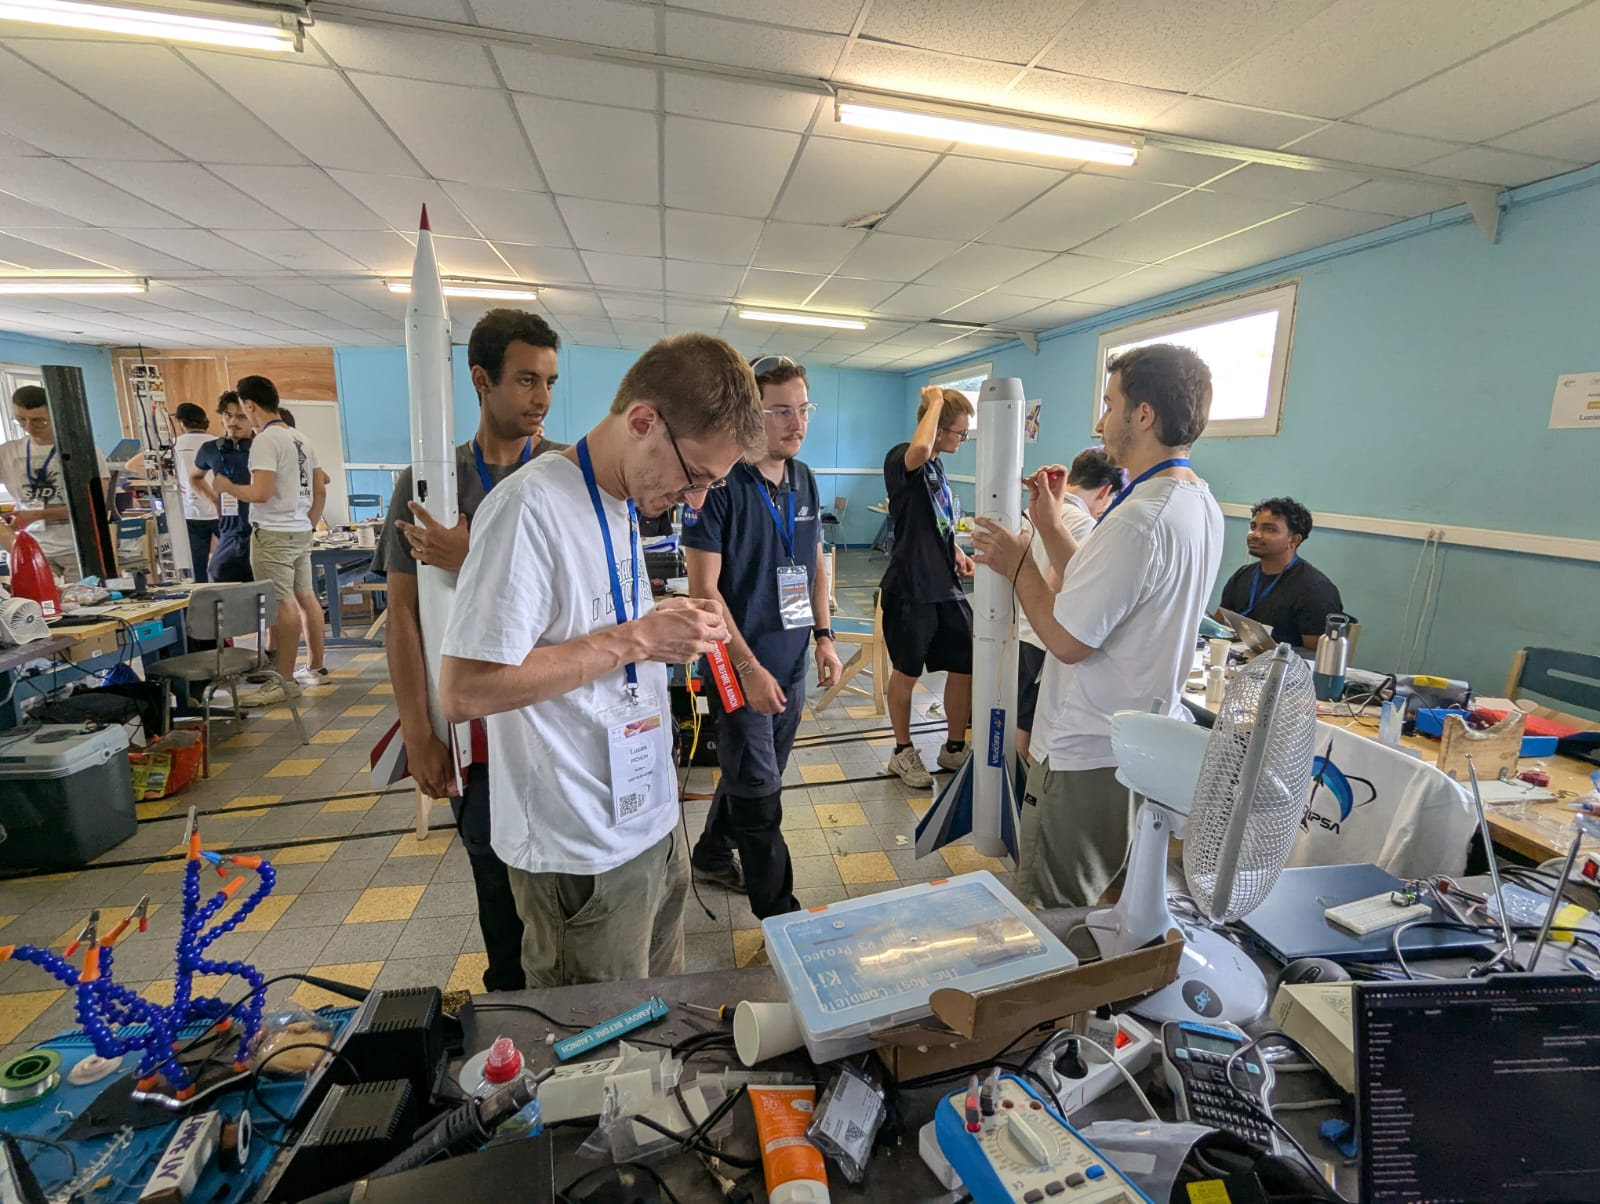
\includegraphics[width=\textwidth]{figures/Montage_club.jpeg}
    \end{subfigure}
    \hfill
    \begin{subfigure}[b]{0.36\textwidth}
        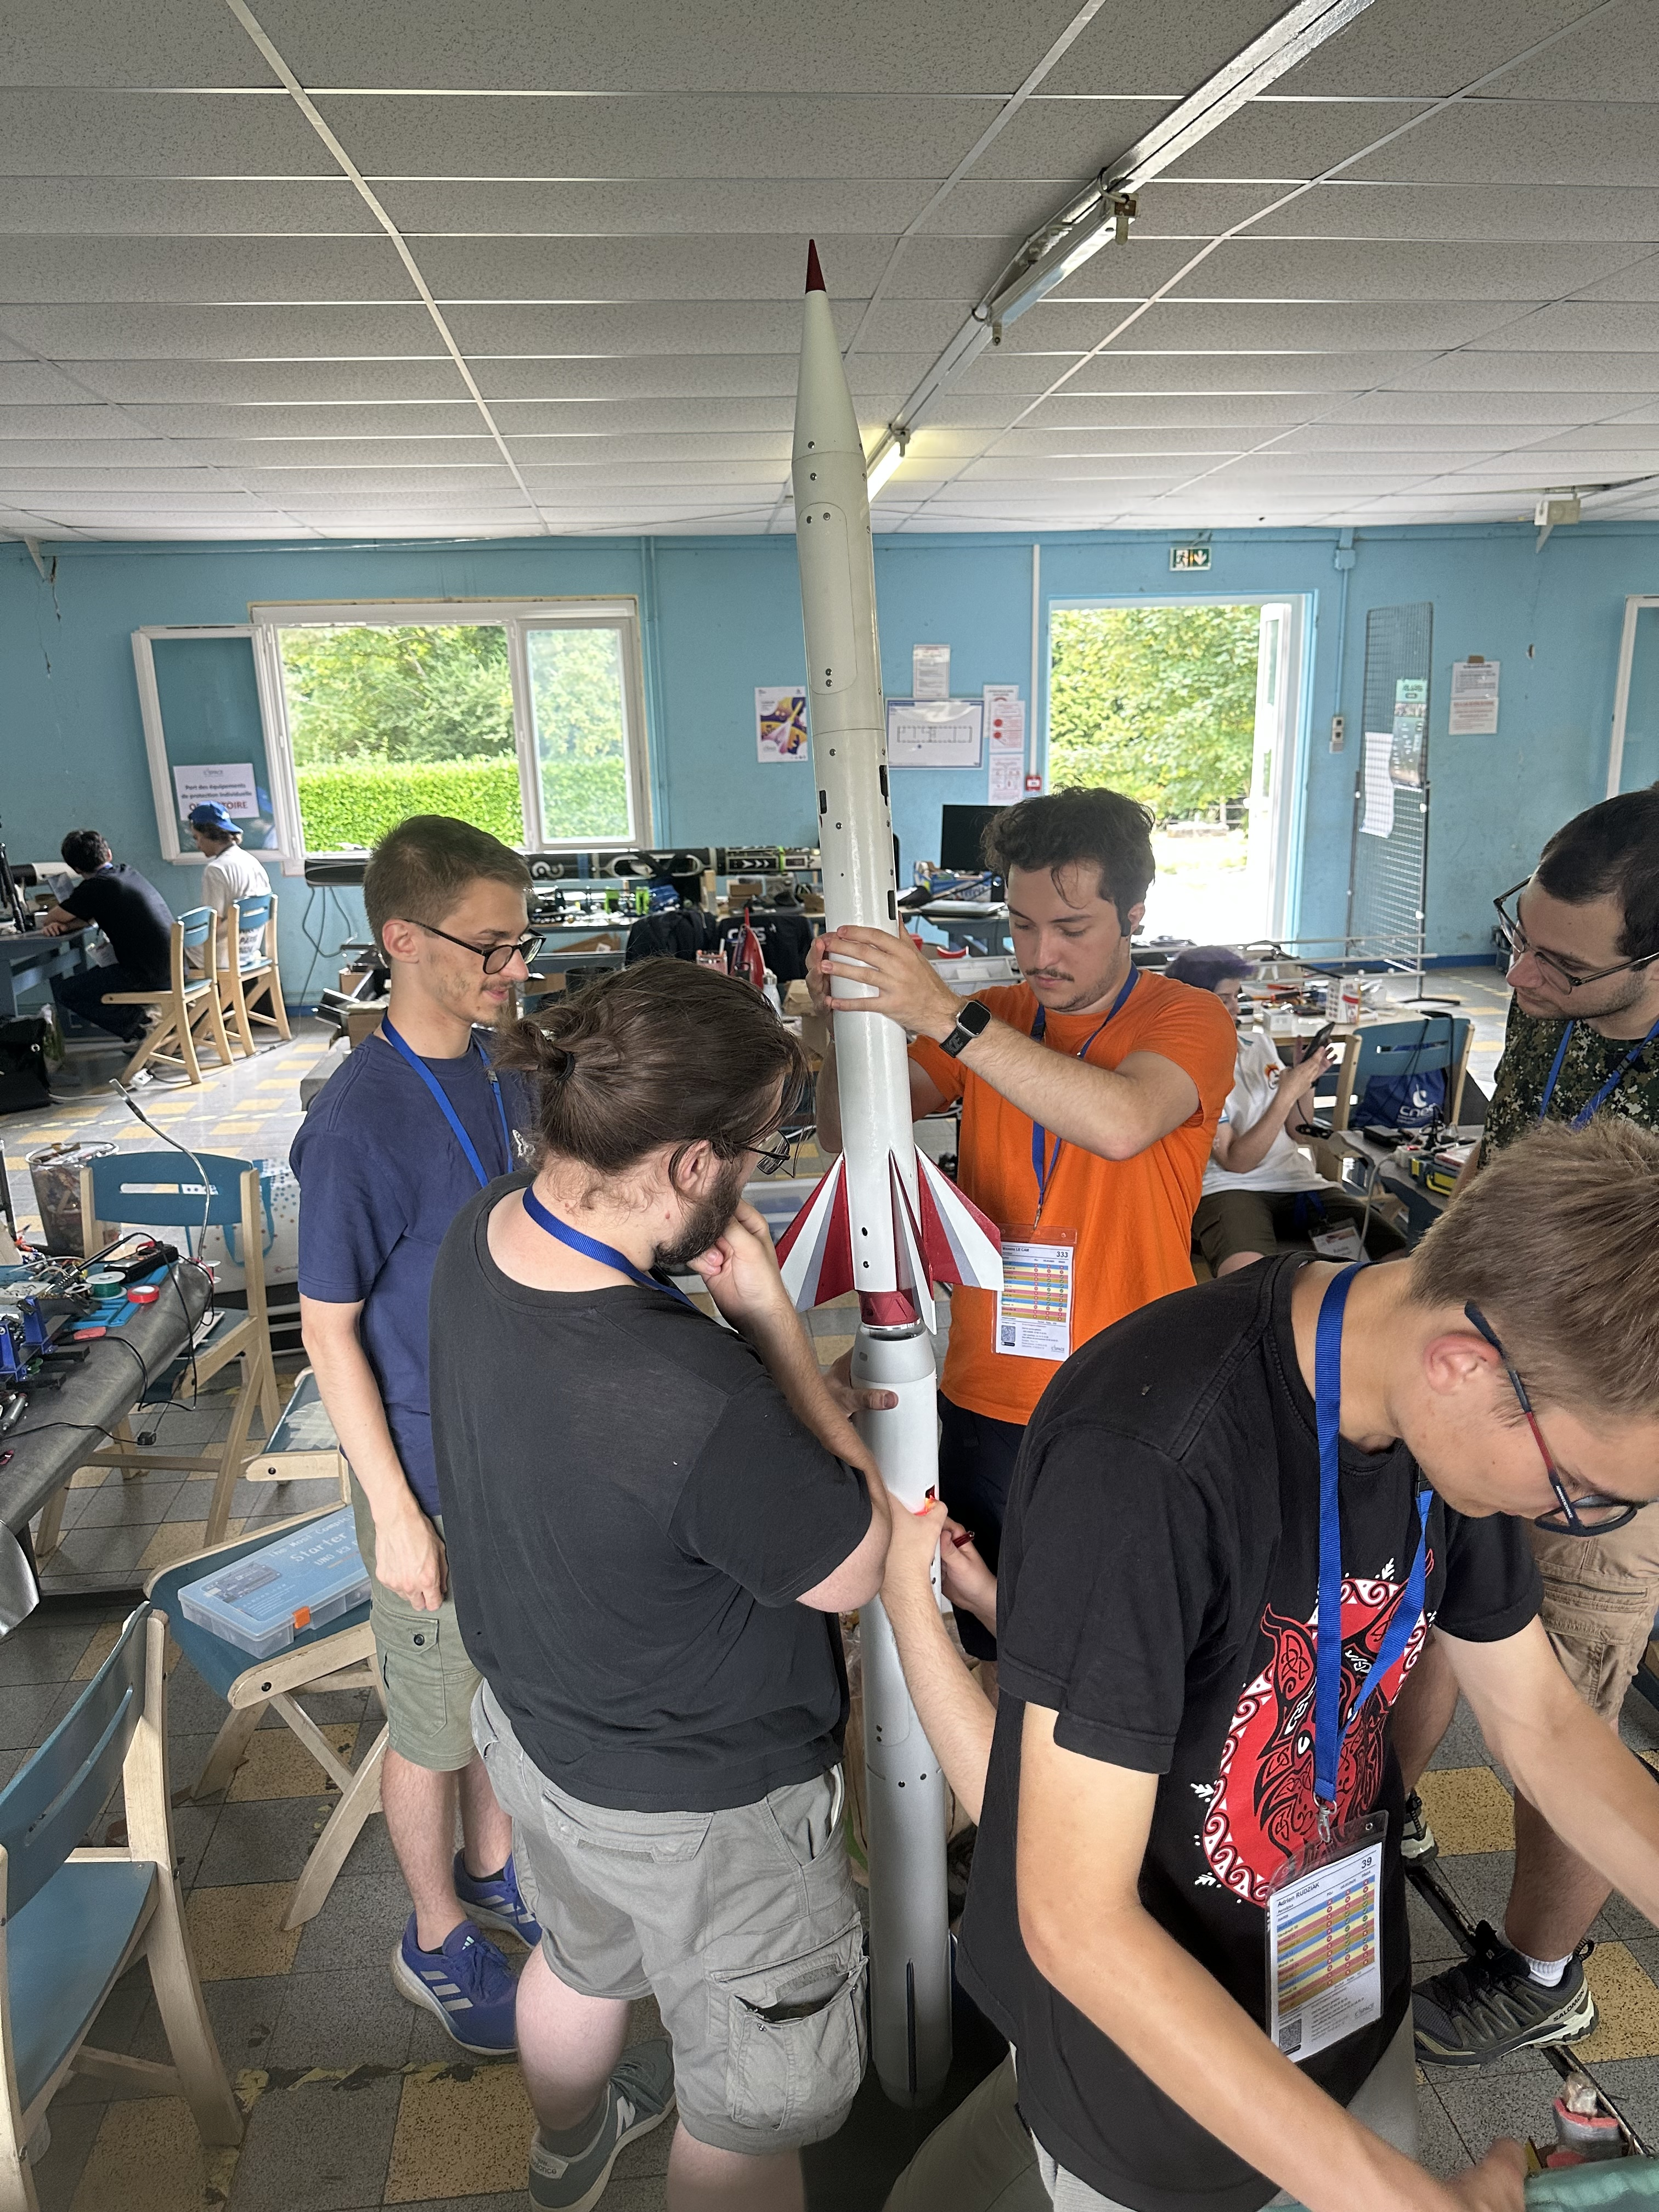
\includegraphics[width=\textwidth]{figures/sp02_controle35.jpg}
    \end{subfigure}
    \caption{Assemblage de la fusée en zone Club}
    \label{fig:montage_club}
\end{figure}

\subsubsection{Lundi : premiers contrôles}
Les premiers contrôles, principalement mécaniques, ont été passés avec succès malgré leur durée exceptionnelle, 
due à la complexité d'une fusée bi-étage. Le test de flèche, point critique pour ce type de structure, a été validé 
du premier coup, sans retouche et avec des marges de sécurité exemplaires. La plupart des systèmes électroniques ont 
également été vérifiés et approuvés.

\begin{figure}[!ht]
    \centering
    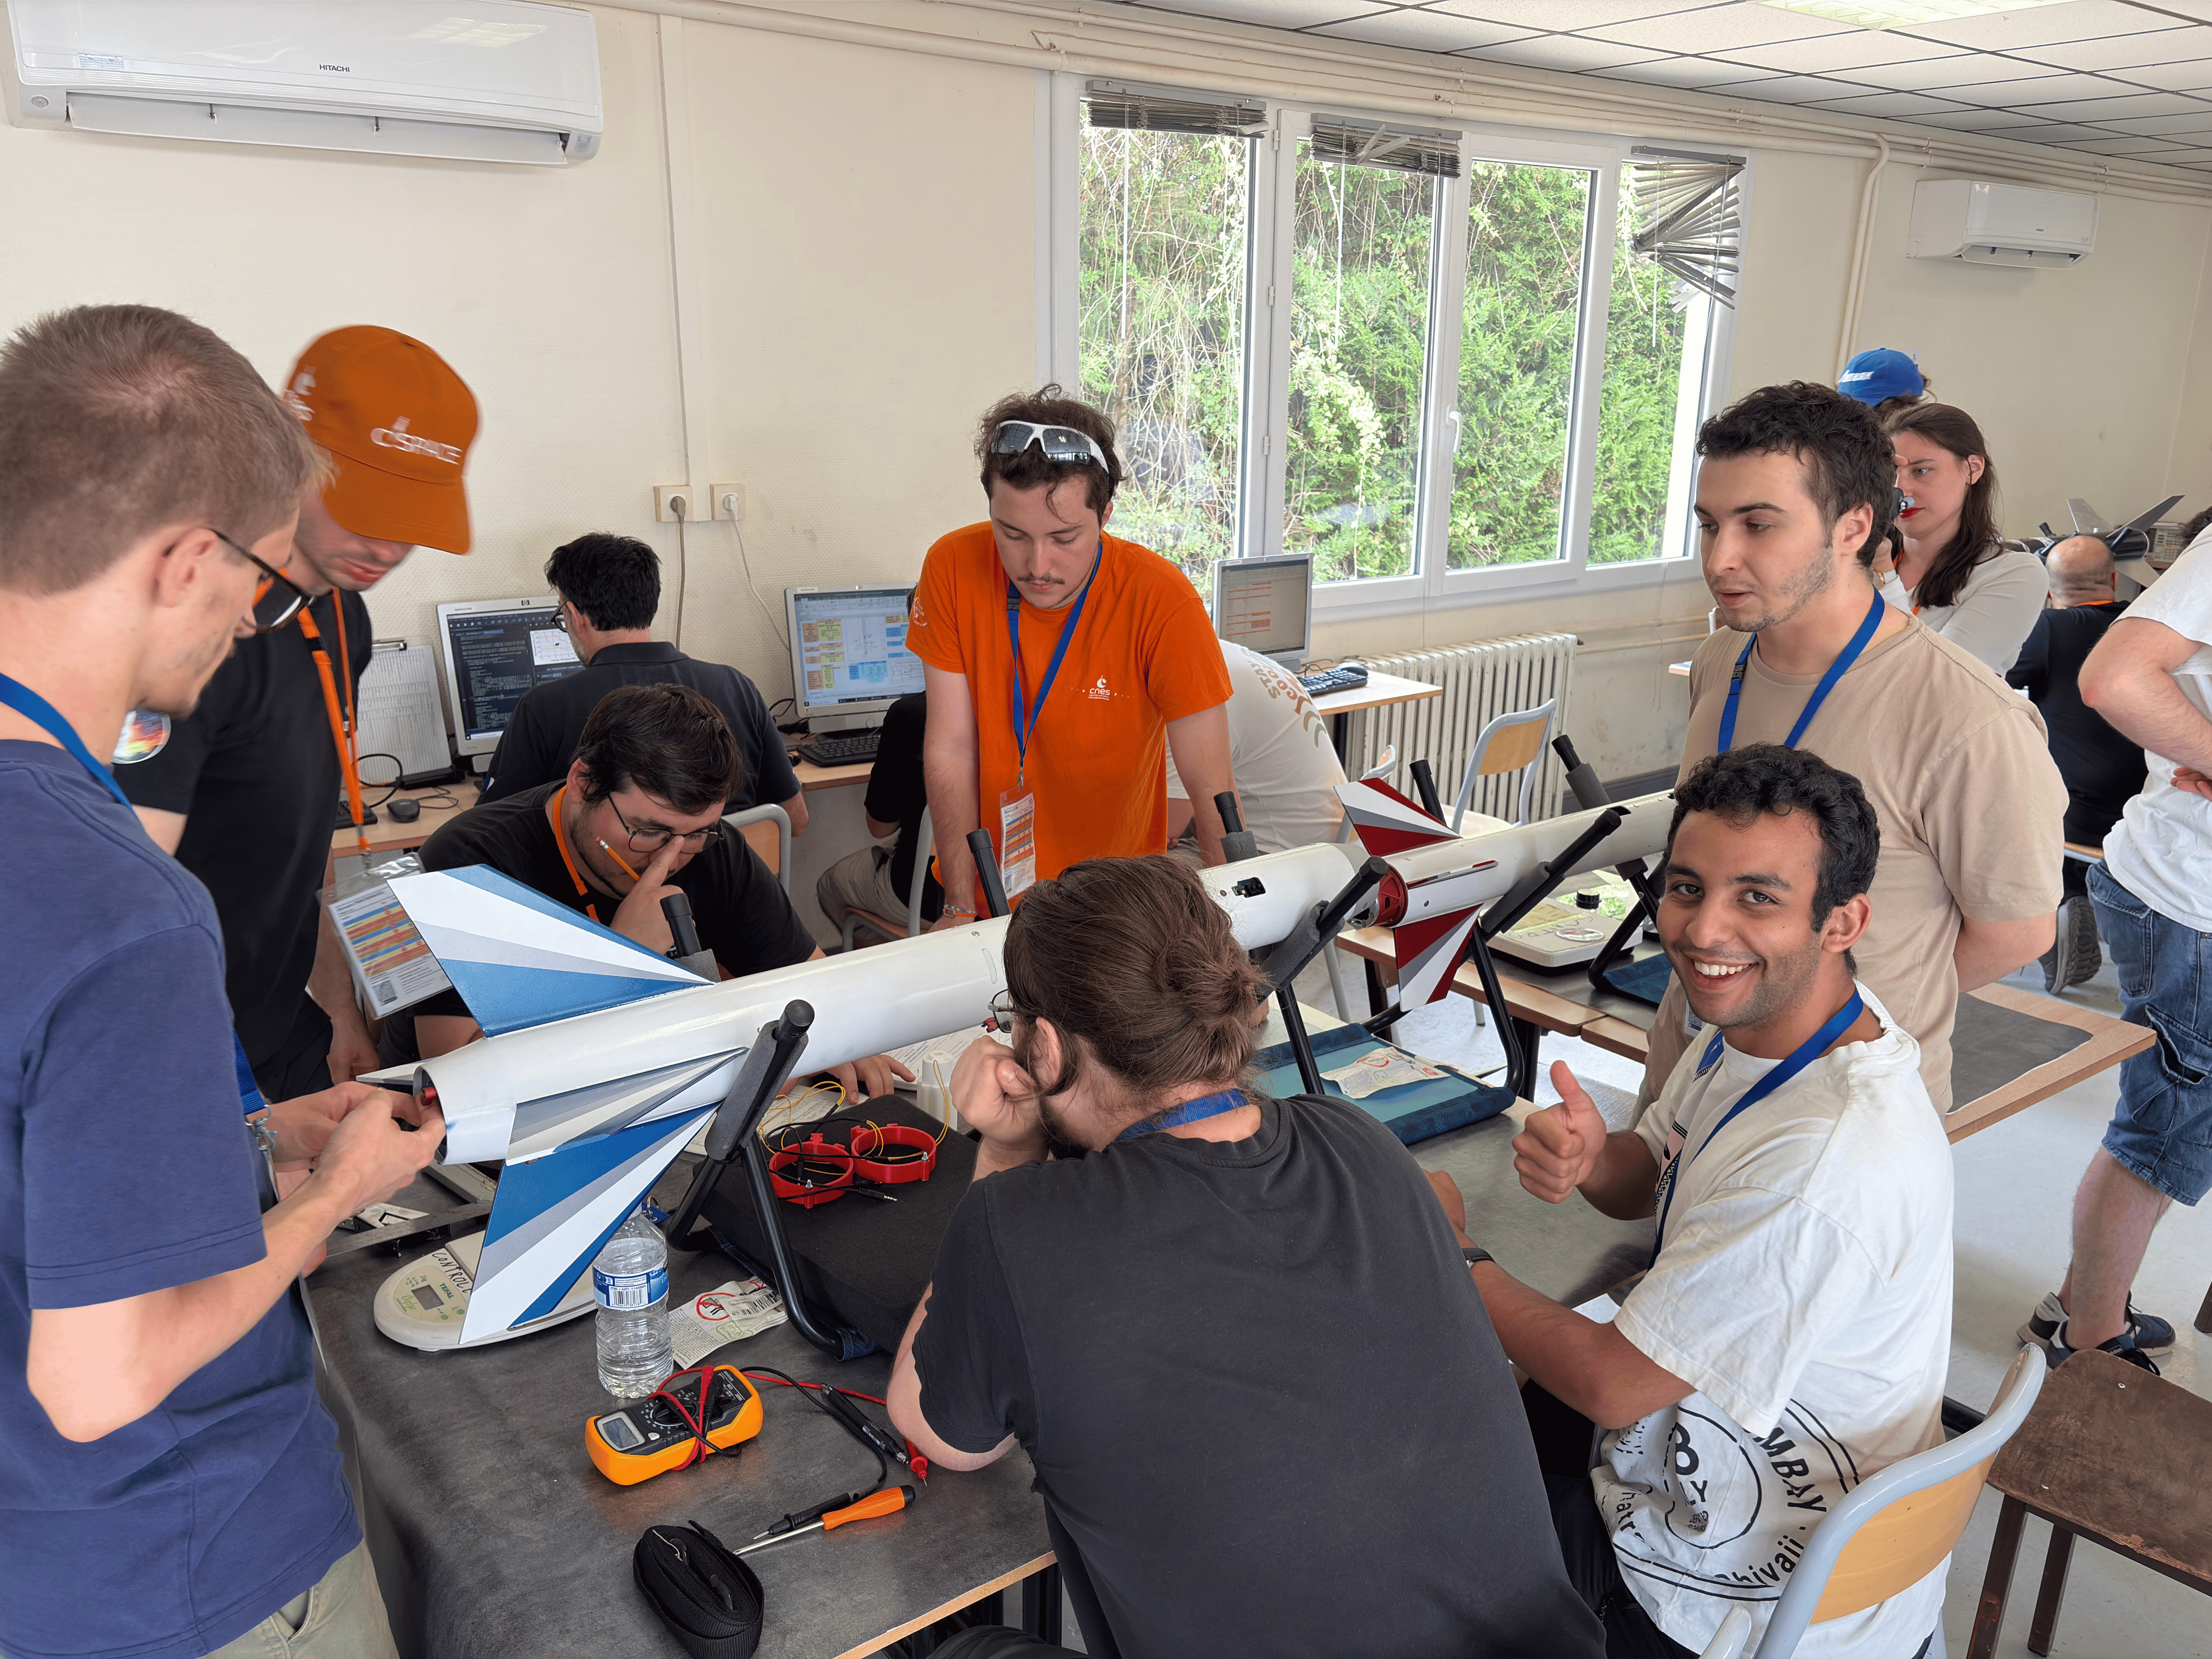
\includegraphics[width=0.5\linewidth]{figures/sp02_controle25.png}
    \caption{Premiers contrôles}
    \label{fig:controle_j1}
\end{figure}

\newpage

\begin{figure}[!ht]
    \centering
    \begin{subfigure}[b]{0.49\textwidth}
        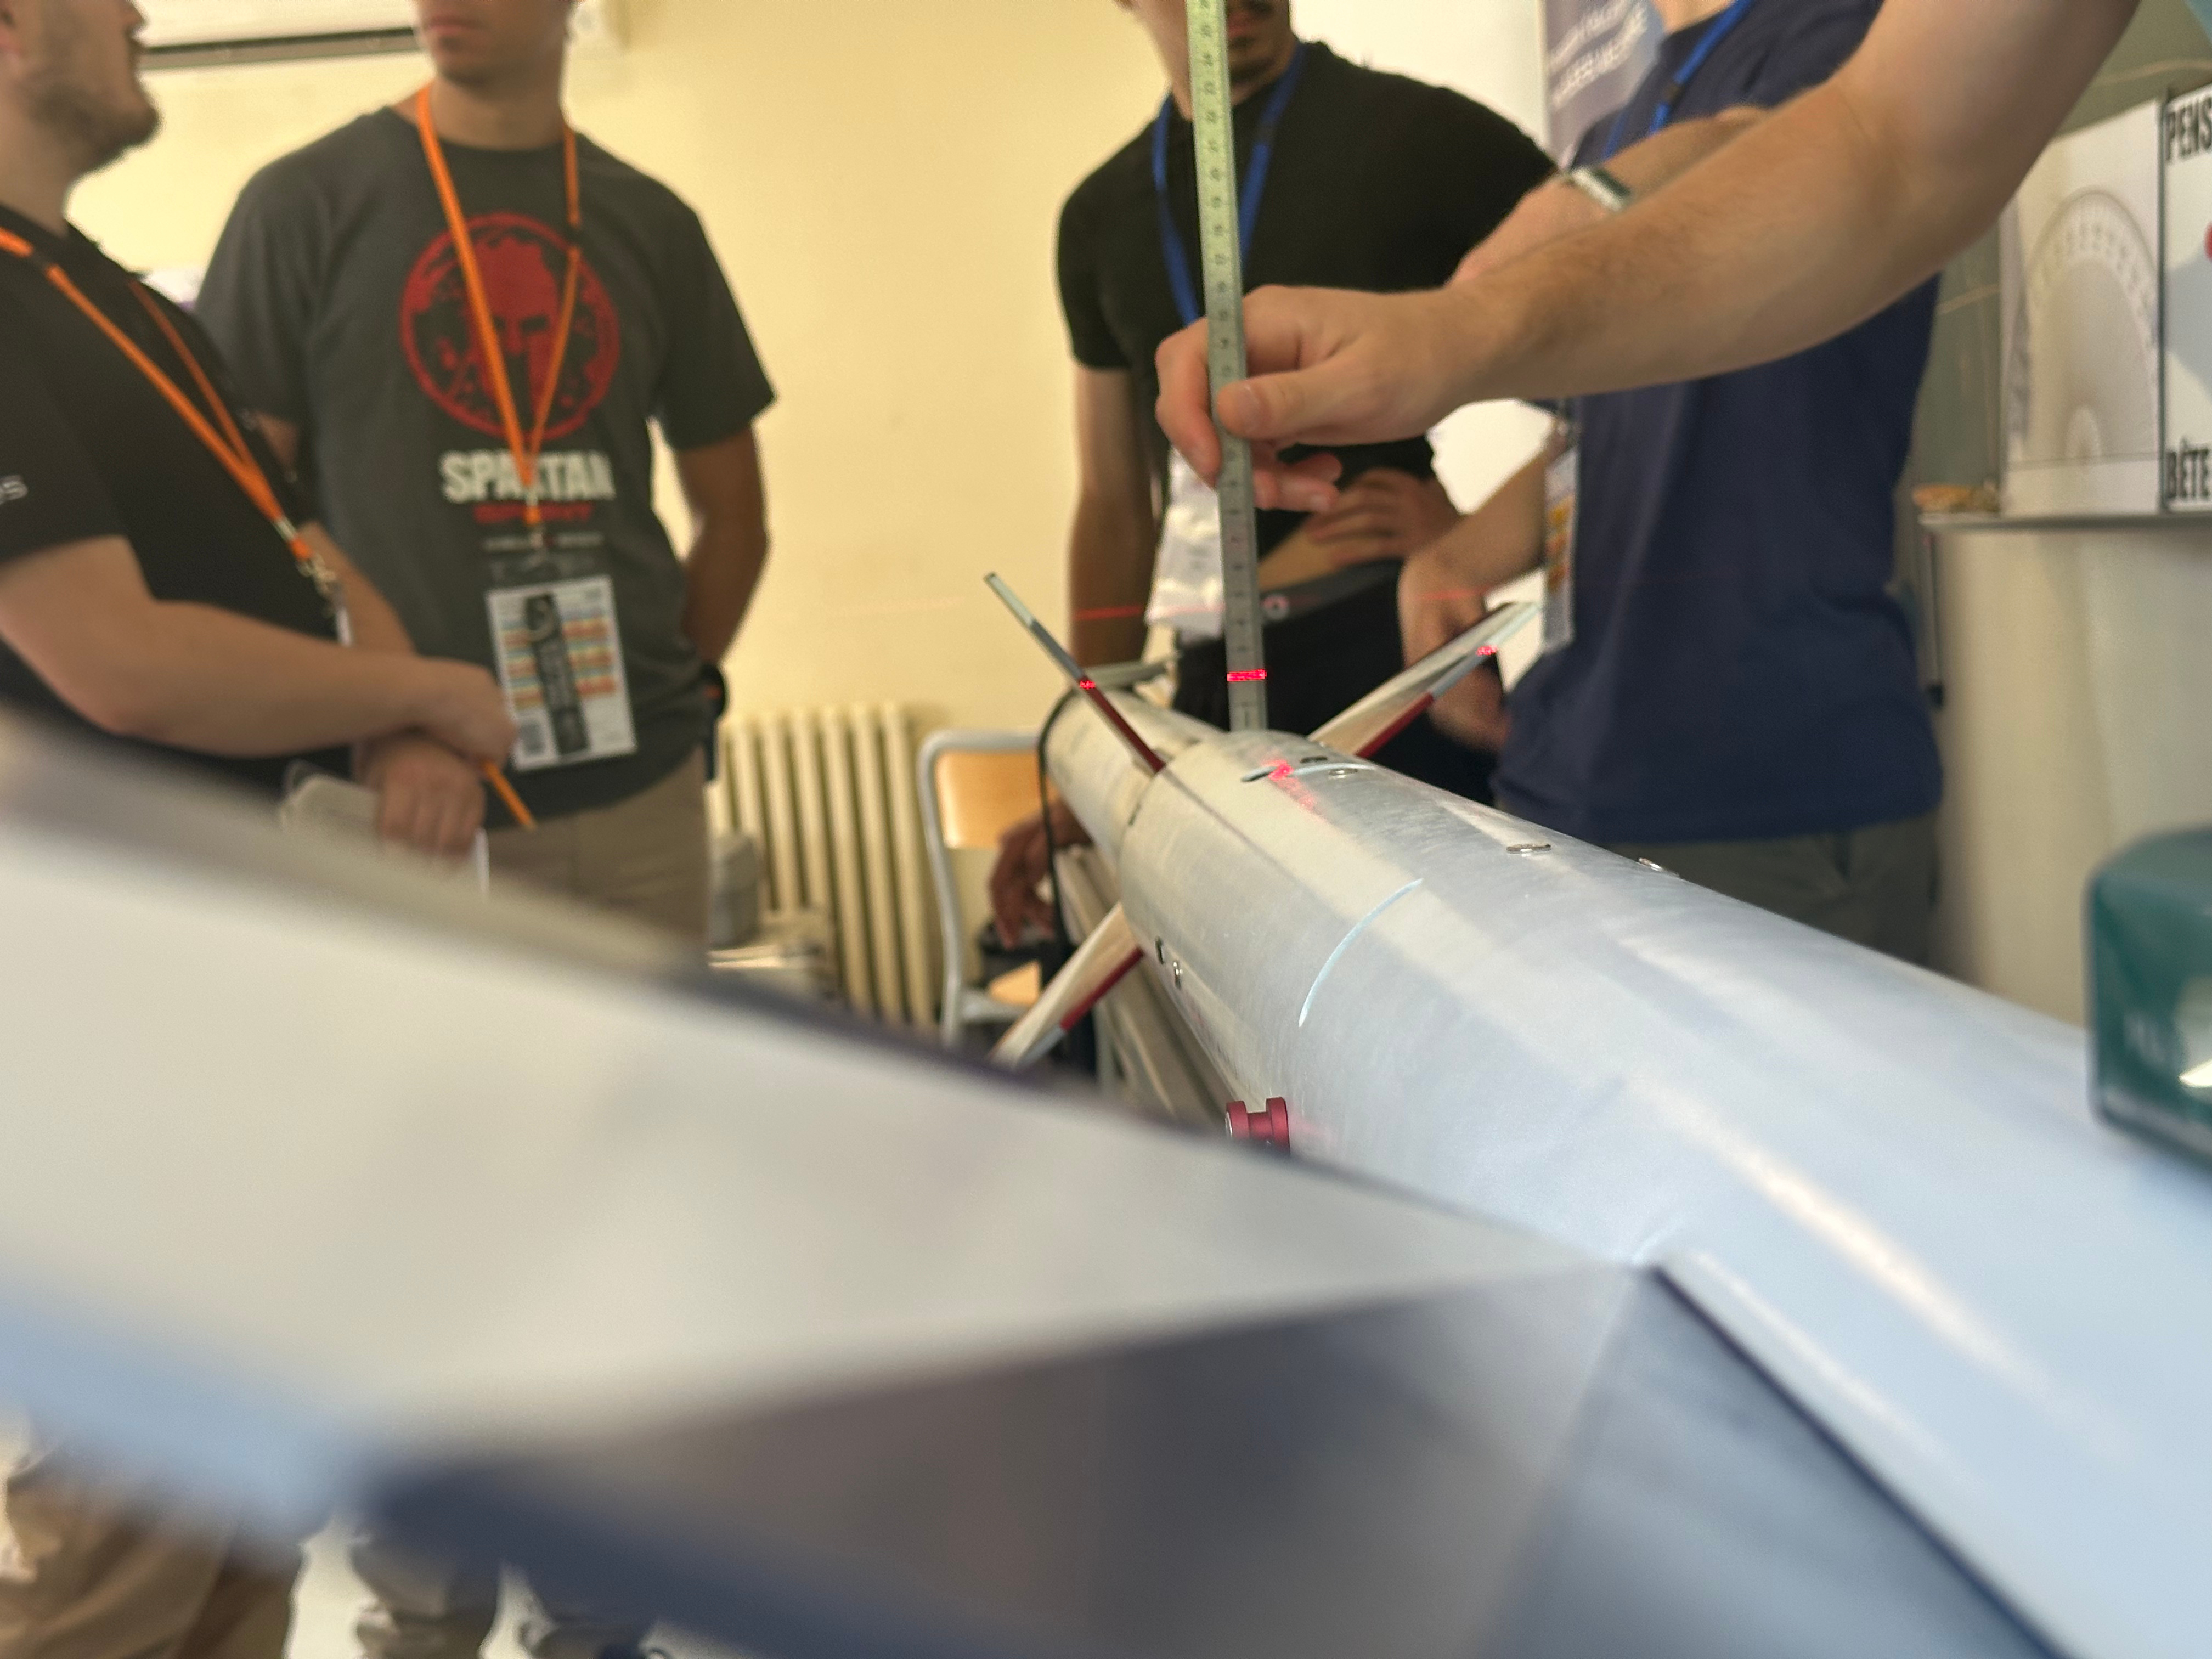
\includegraphics[width=\textwidth]{figures/sp02_controle18.png}
    \end{subfigure}
    \hfill
    \begin{subfigure}[b]{0.49\textwidth}
        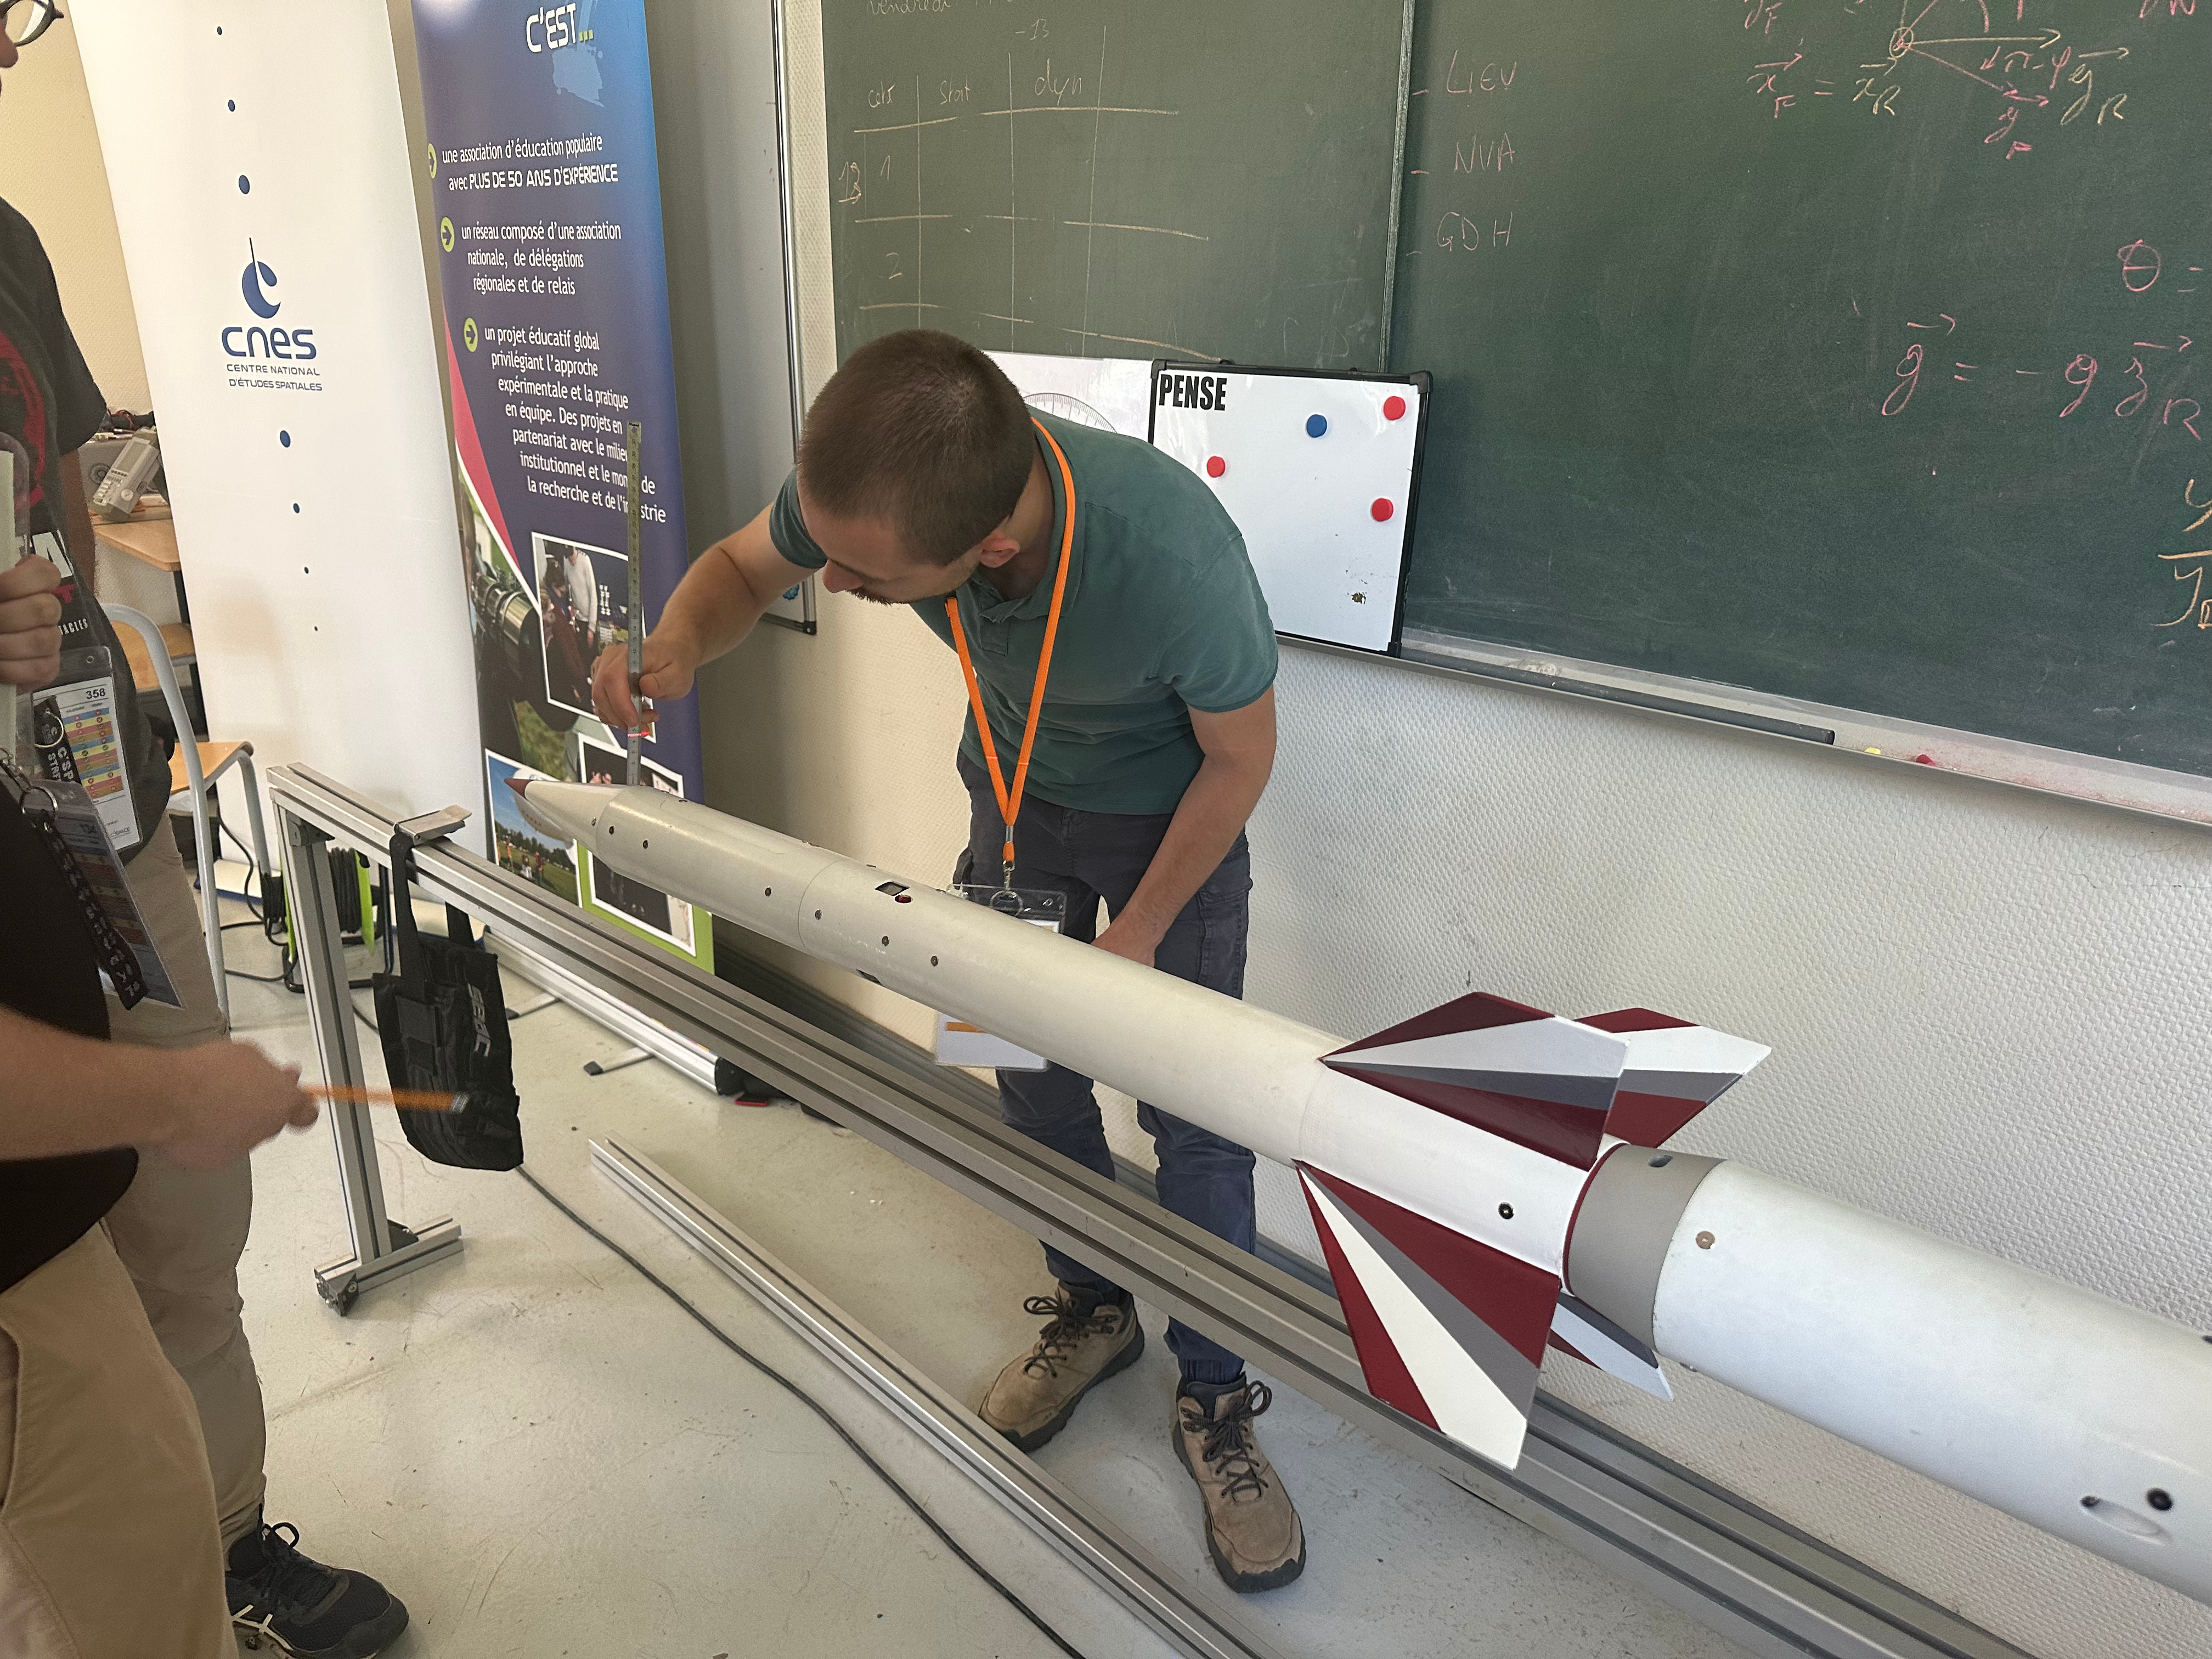
\includegraphics[width=\textwidth]{figures/sp02_controle22.png}
    \end{subfigure}
    \caption{Contrôle de la flèche}
    \label{fig:controle_j2}
\end{figure}

\begin{figure}[!ht]
    \centering
    \begin{subfigure}[b]{0.32\textwidth}
        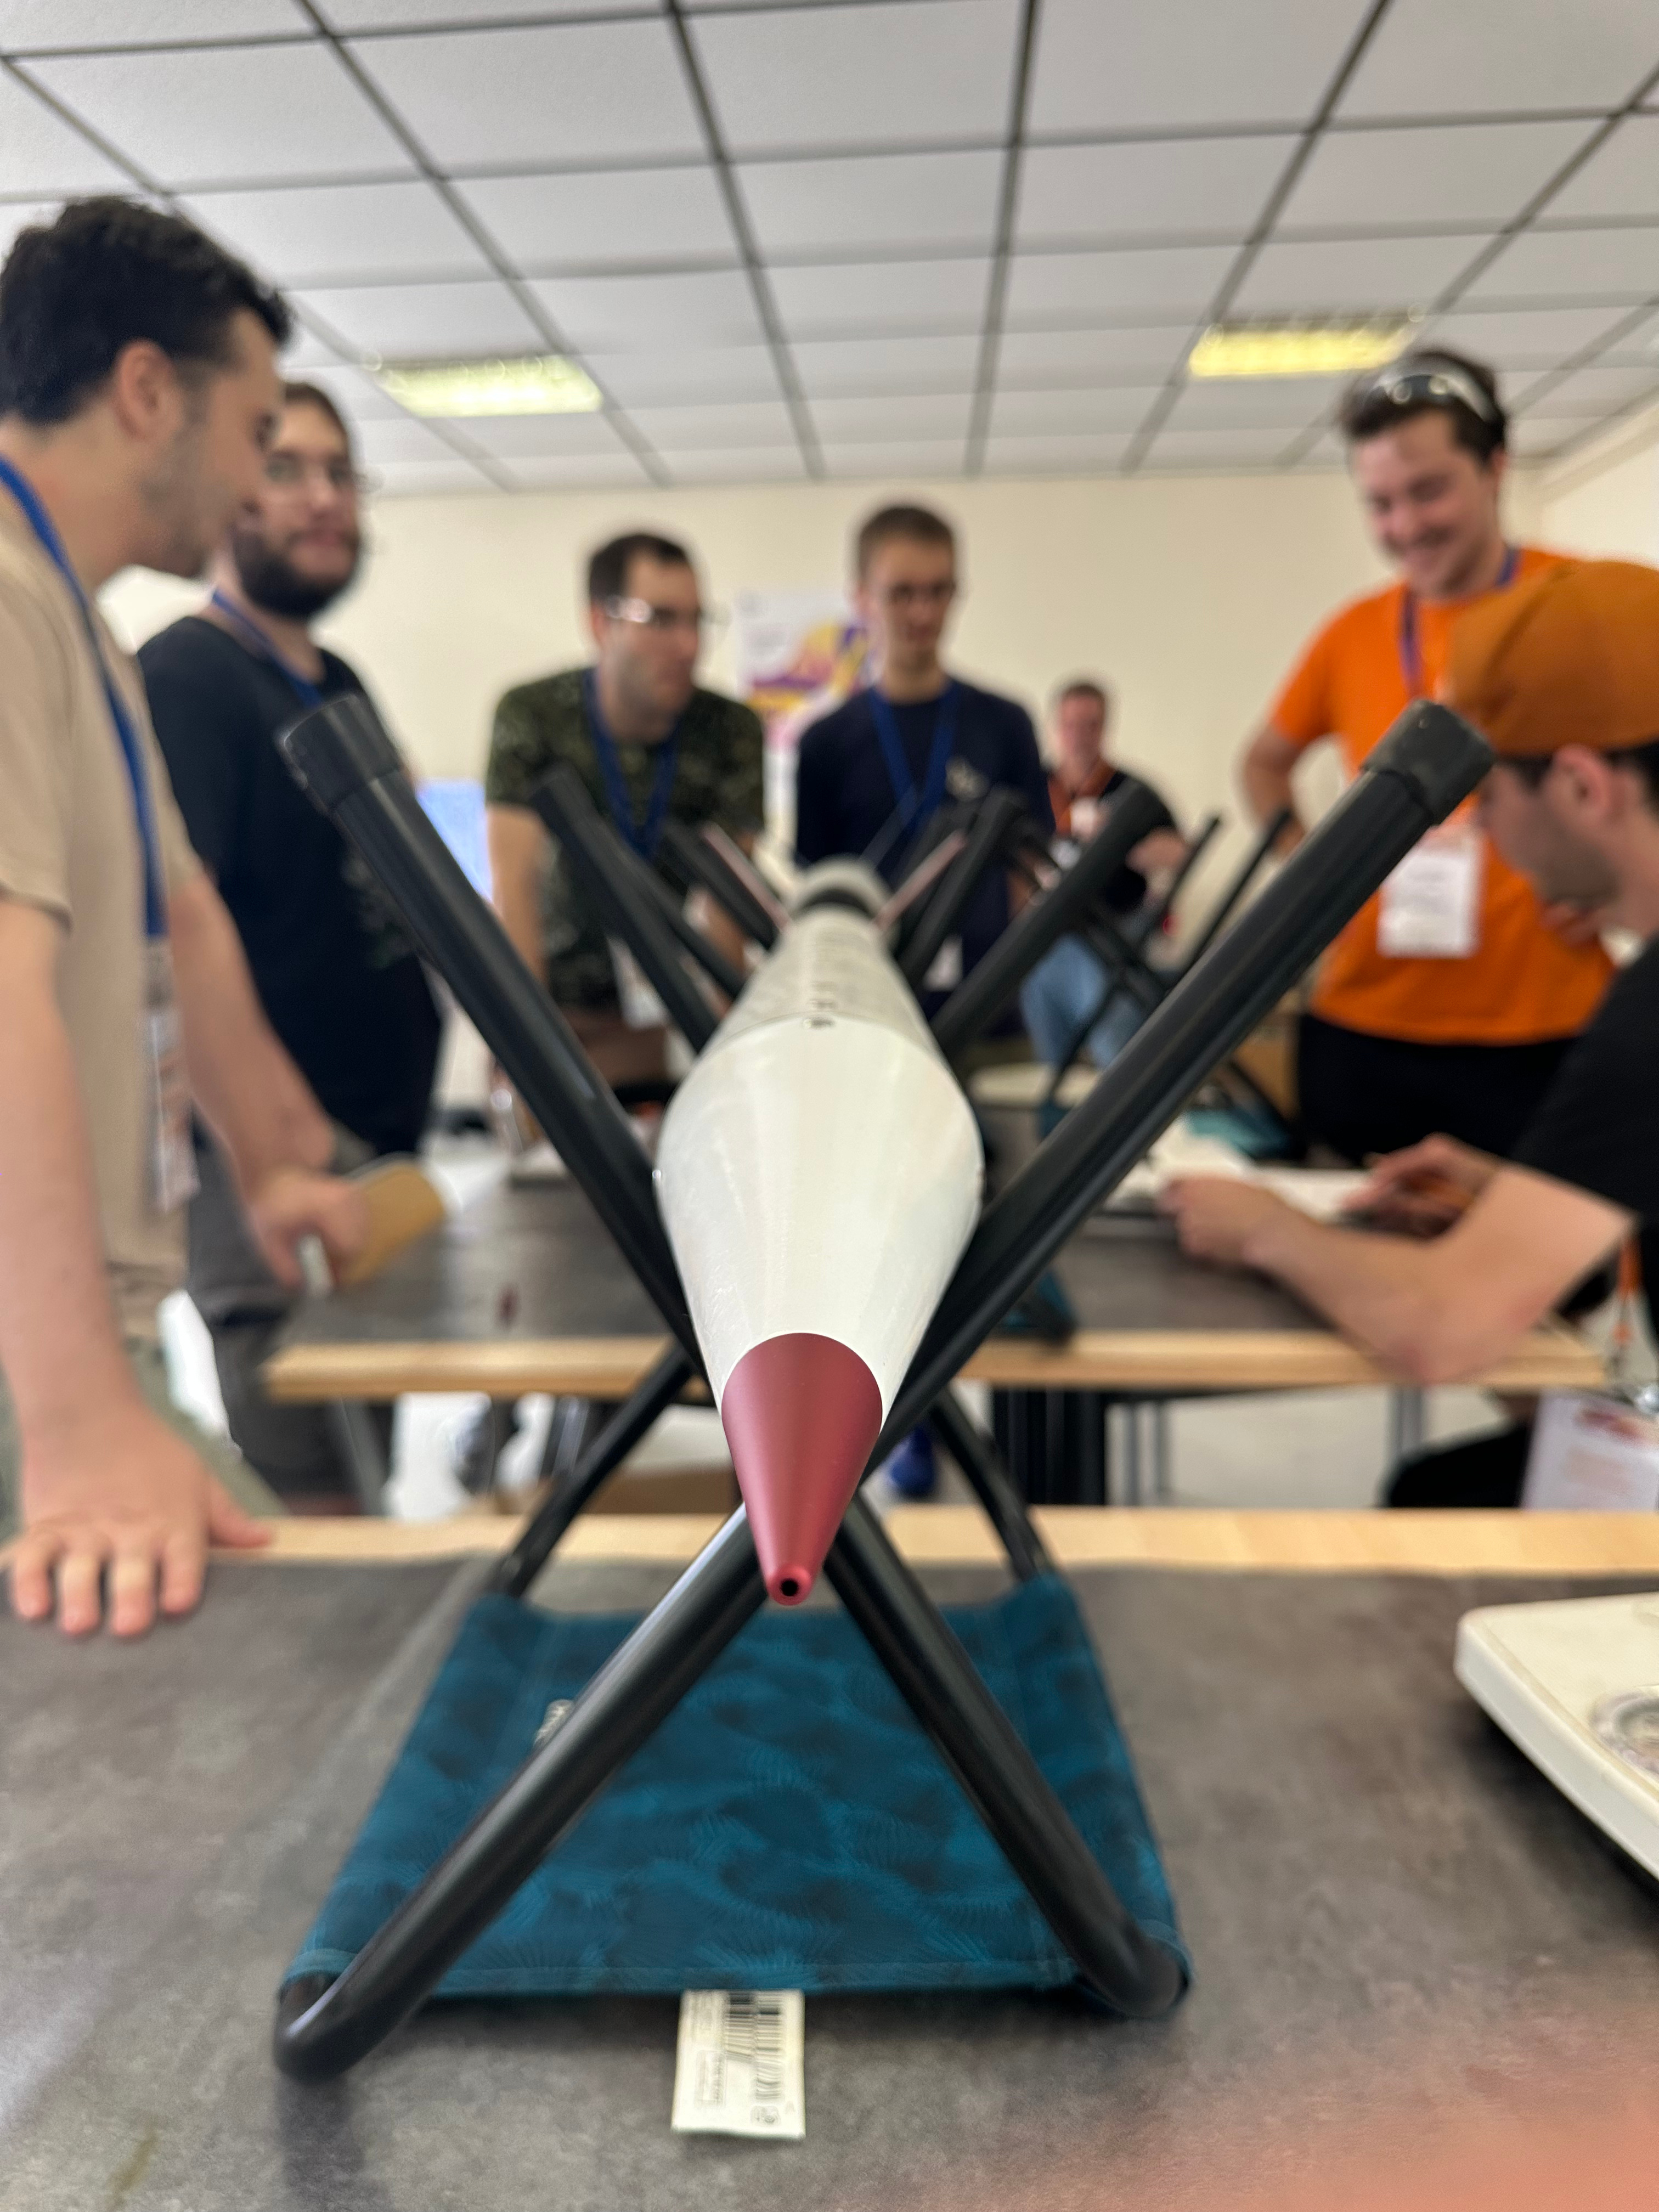
\includegraphics[width=\textwidth]{figures/sp02_controle9.png}
    \end{subfigure}
    \hfill
    \begin{subfigure}[b]{0.32\textwidth}
        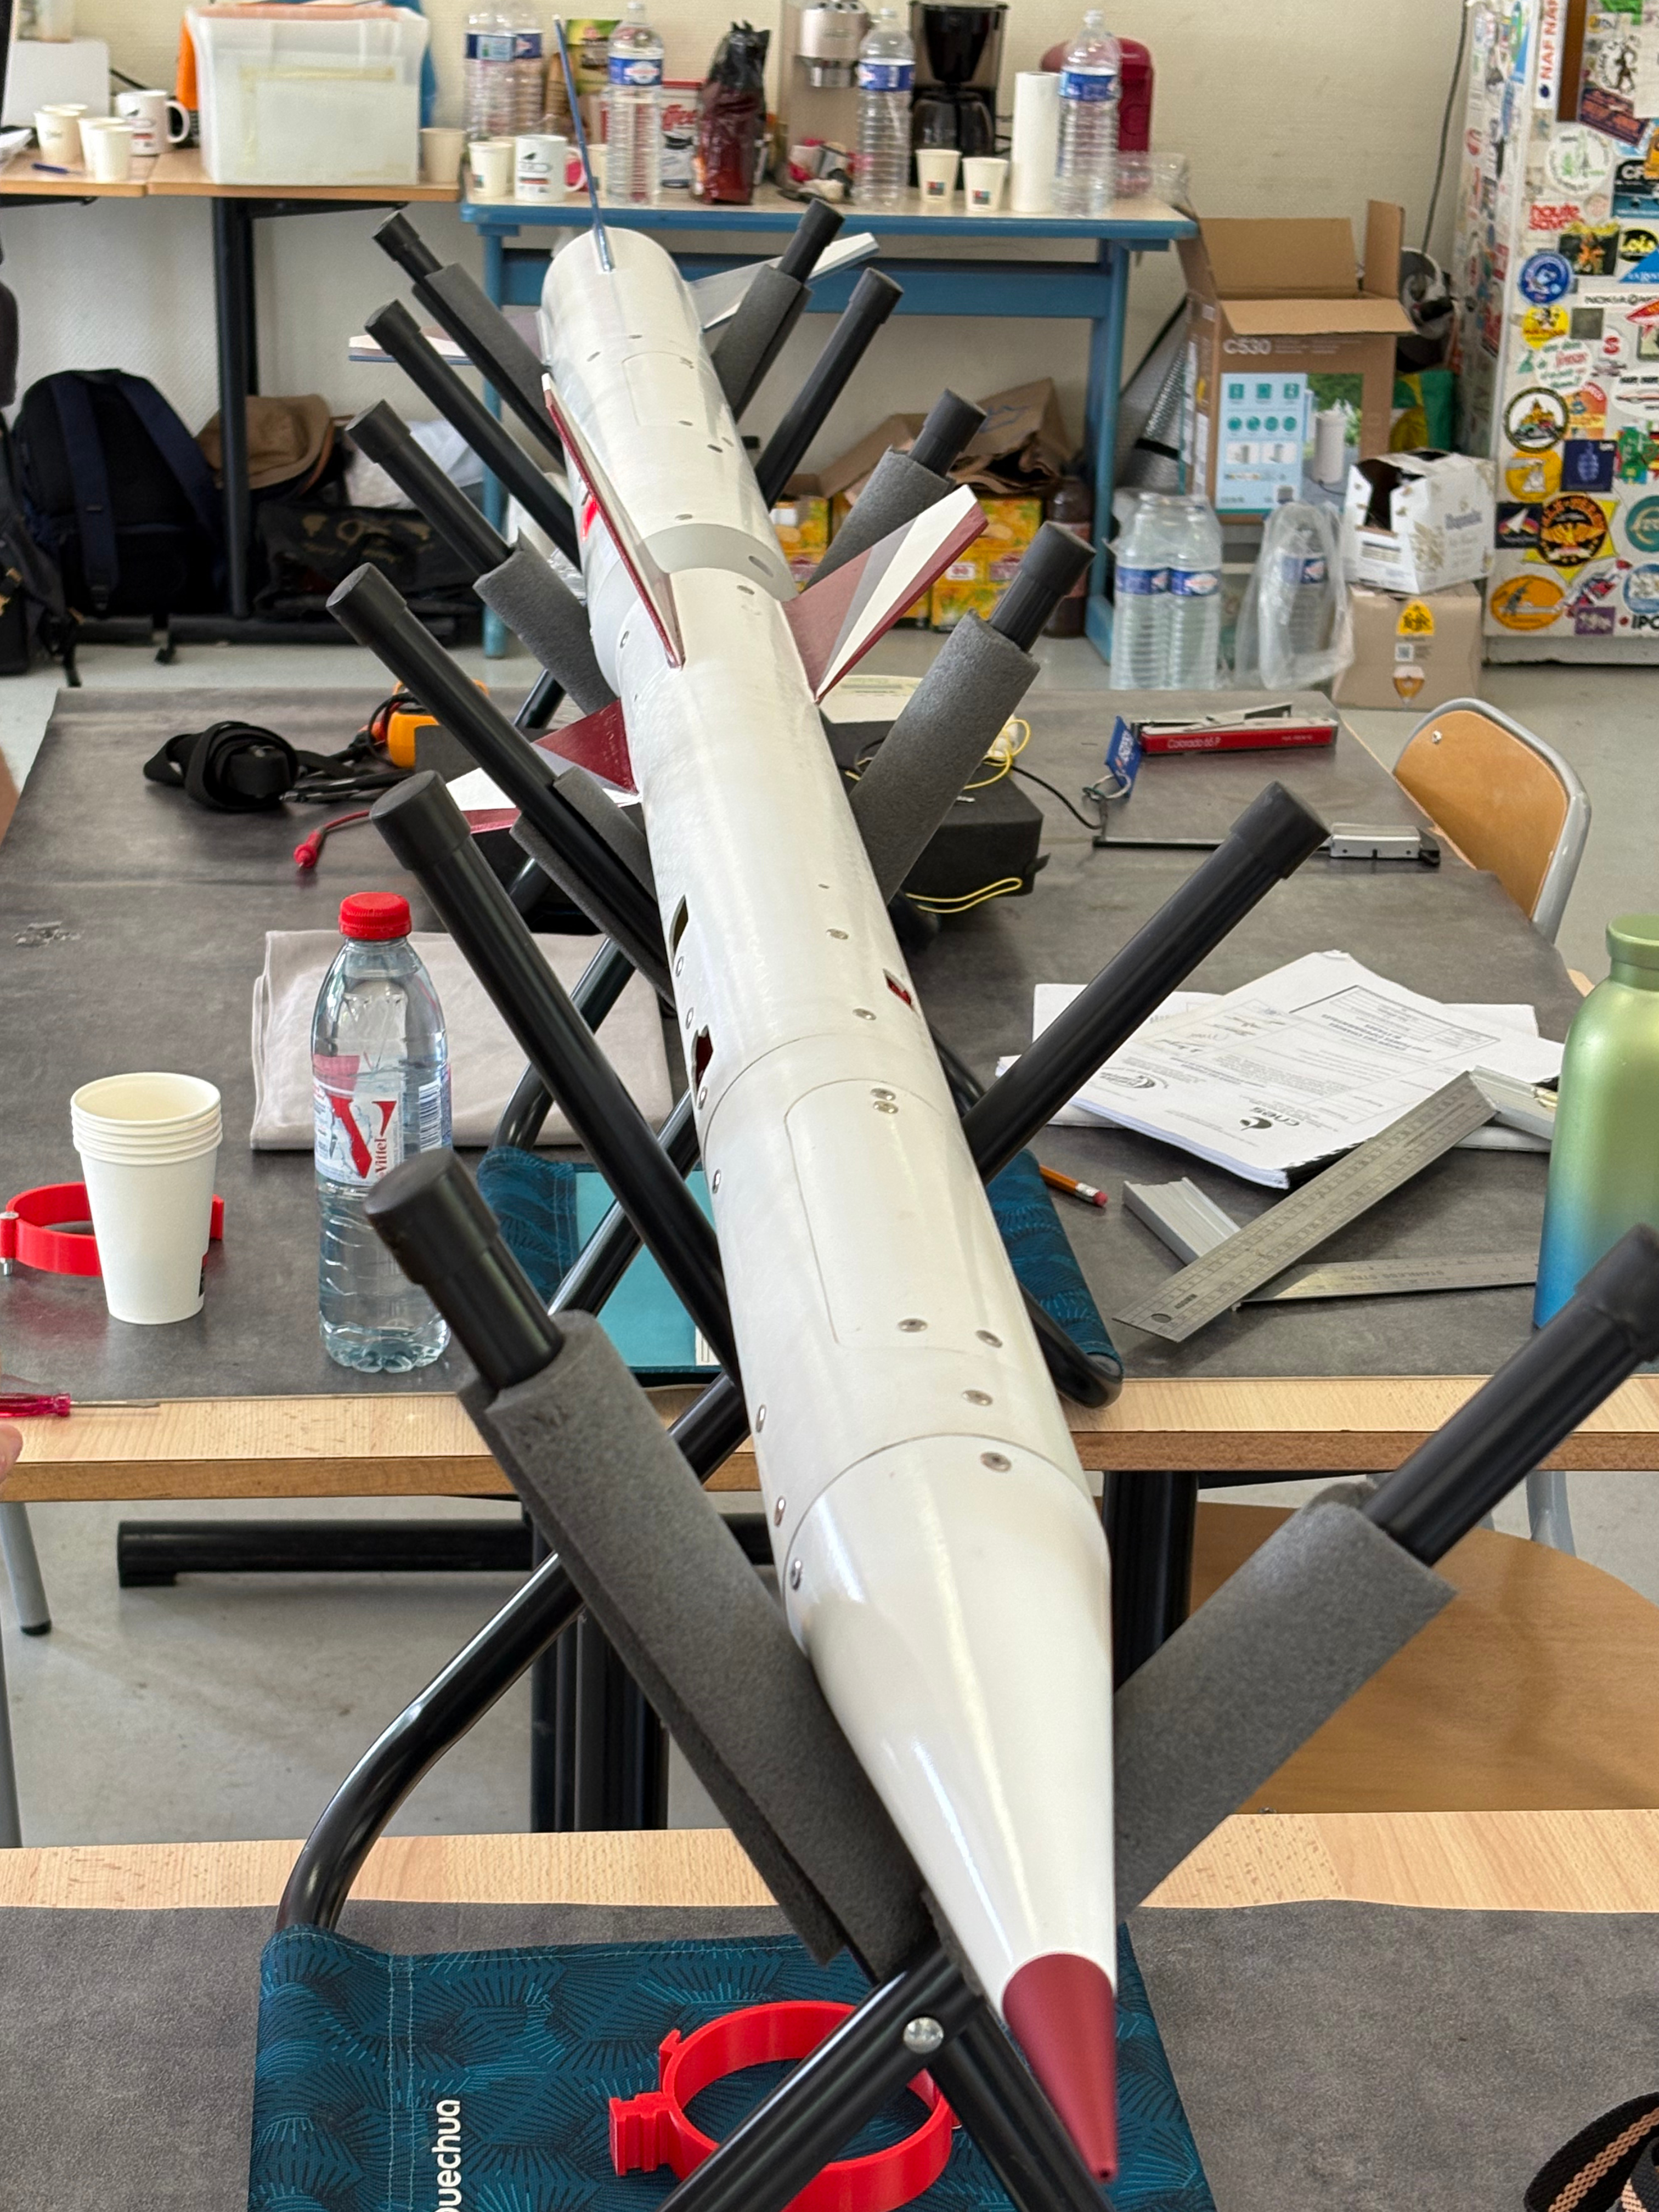
\includegraphics[width=\textwidth]{figures/sp02_controle11.png}
    \end{subfigure}
    \hfill
    \begin{subfigure}[b]{0.32\textwidth}
        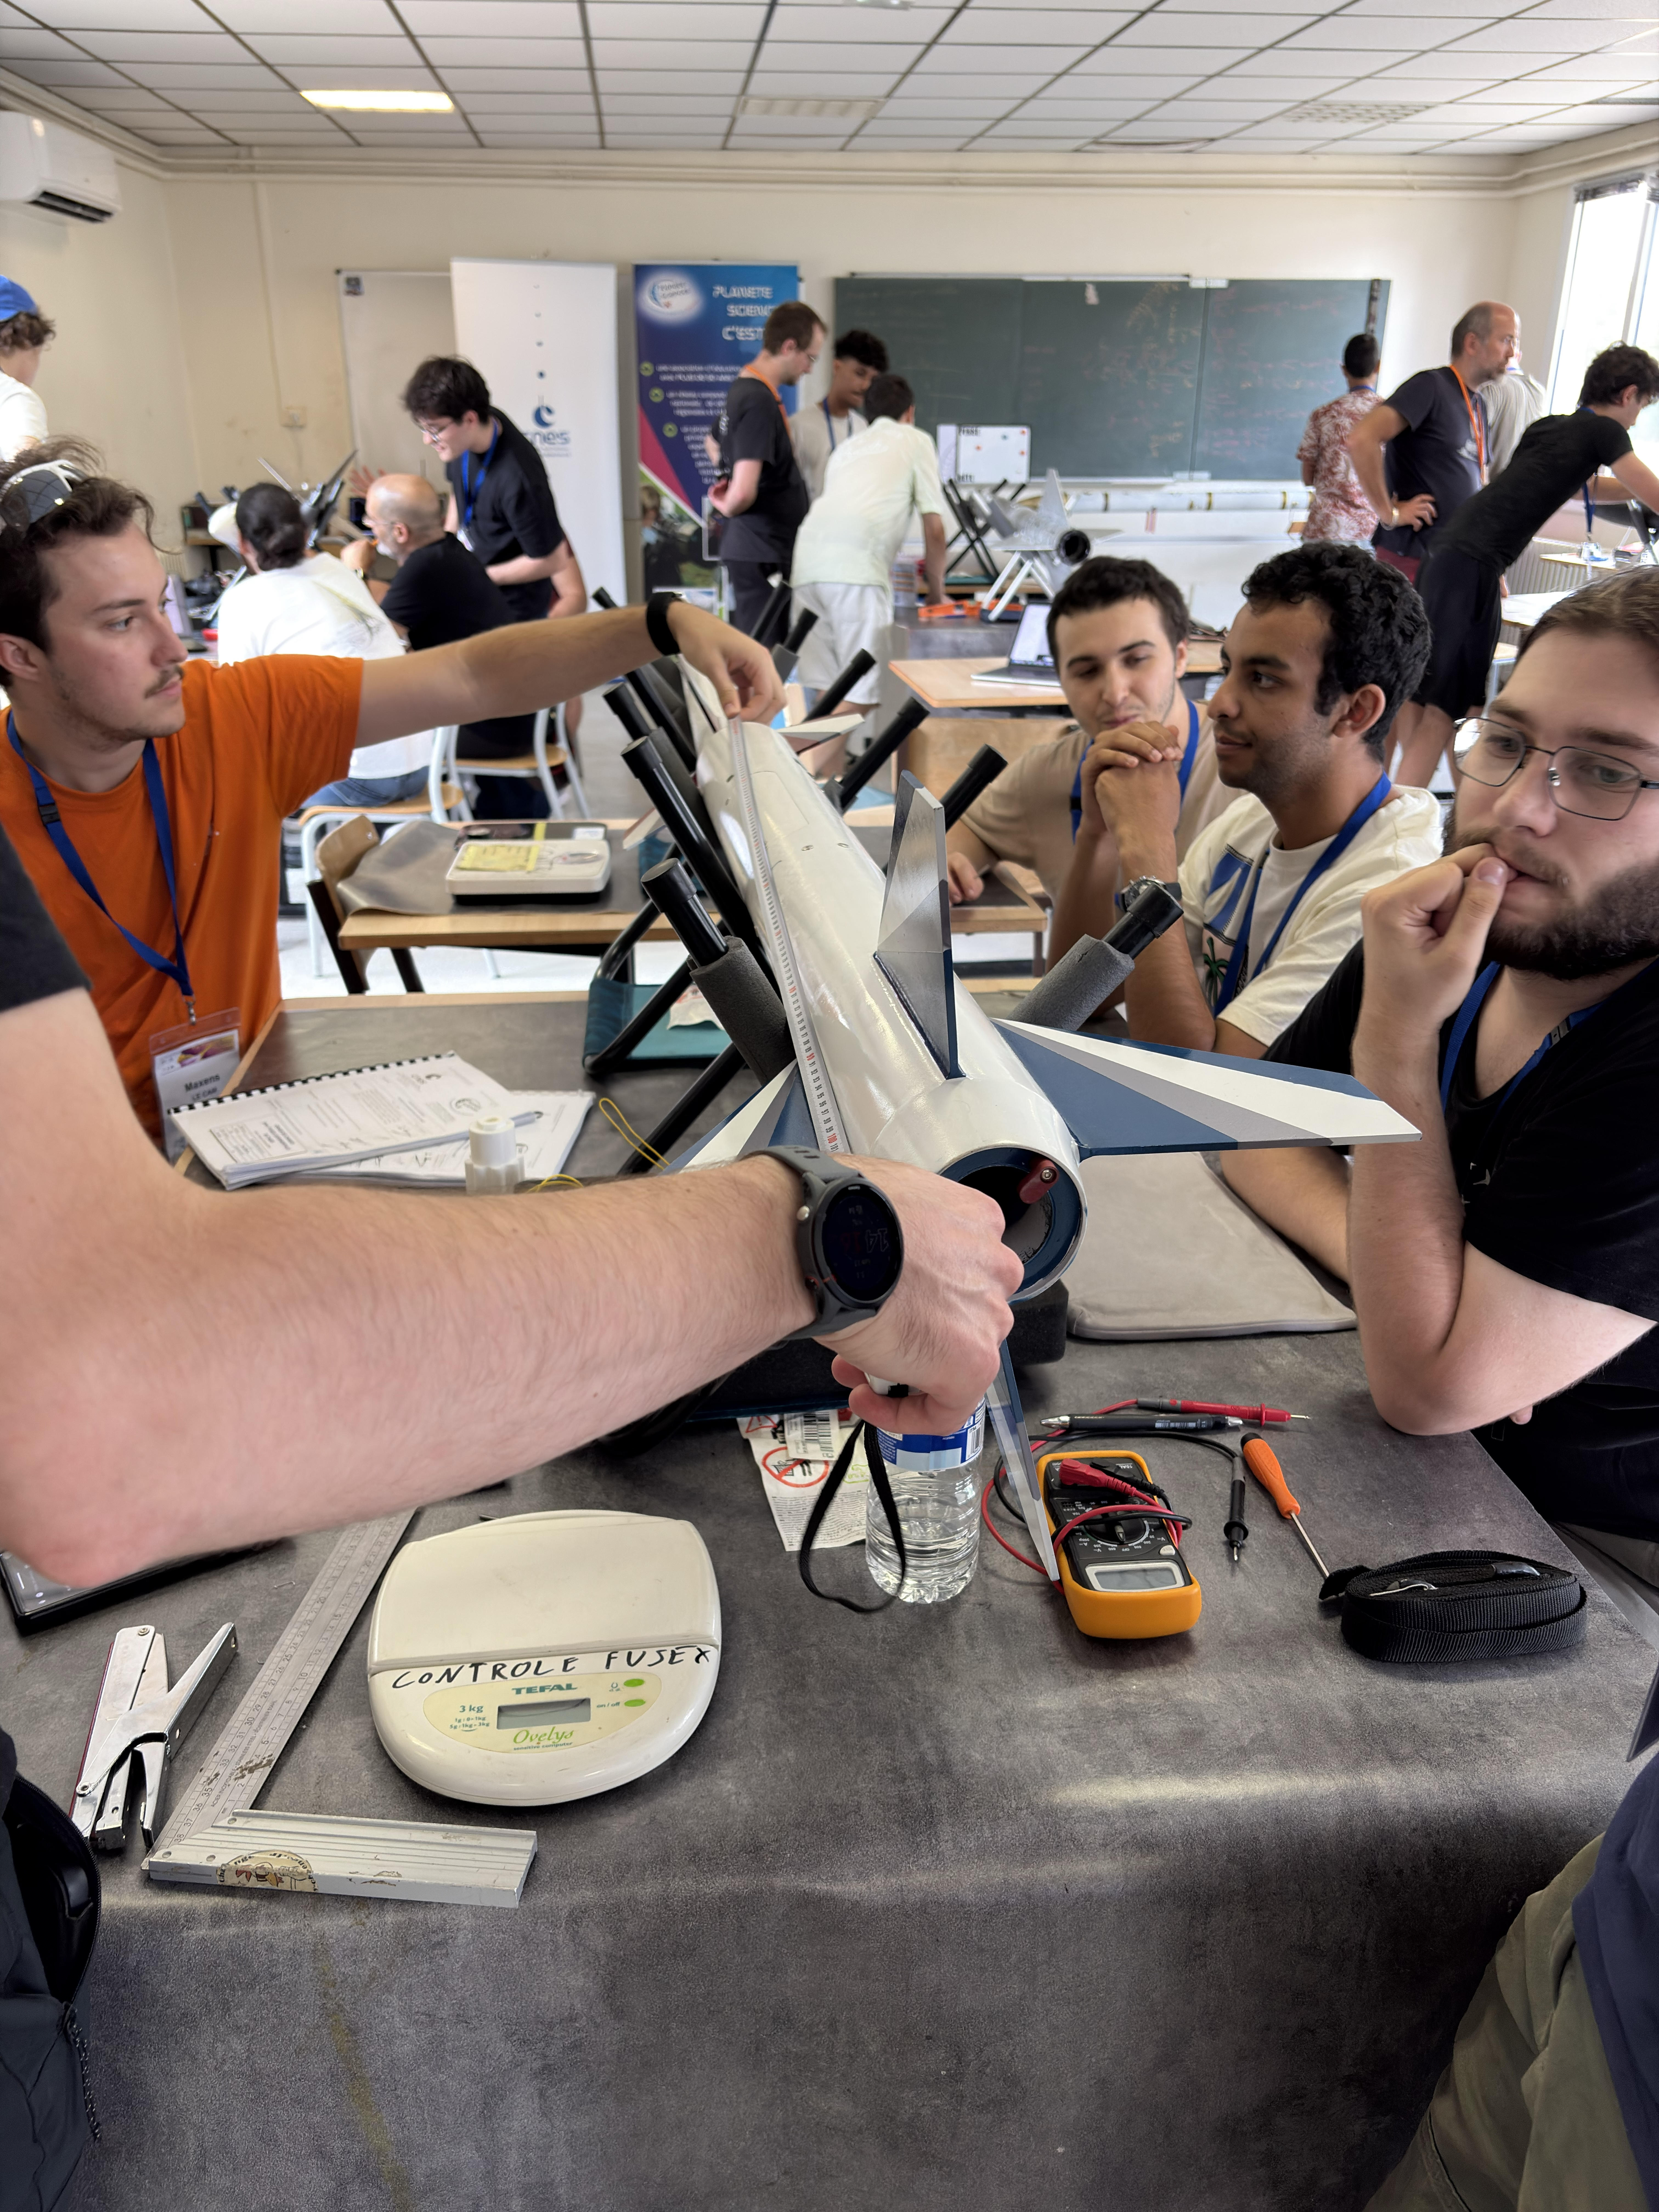
\includegraphics[width=\textwidth]{figures/sp02_controle37.jpg}
    \end{subfigure}
    \caption{Poursuite des contrôles mécaniques}
    \label{fig:controle_j2.2}
\end{figure}

\subsubsection{Mardi : adaptation et apprentissage}
Après avoir travaillé sur le deuxième étage, l'équipe a dû remonter entièrement la fusée en un temps record pour 
une compatibilité rampe, décidée tardivement. Bien que cette rampe se soit avérée trop longue et ait posé des problèmes 
lors de l'assemblage, elle a permis d'expérimenter un pseudo-lancement. Cela a inclus la mise en rampe 
de la fusée, les discussions avec les pyrotechniciens, et une leçon inattendue : \textit{la peinture blanche n'est pas 
adaptée pour maintenir une fusée propre}.

\begin{figure}[!ht]
    \centering
    \begin{subfigure}[b]{0.32\textwidth}
        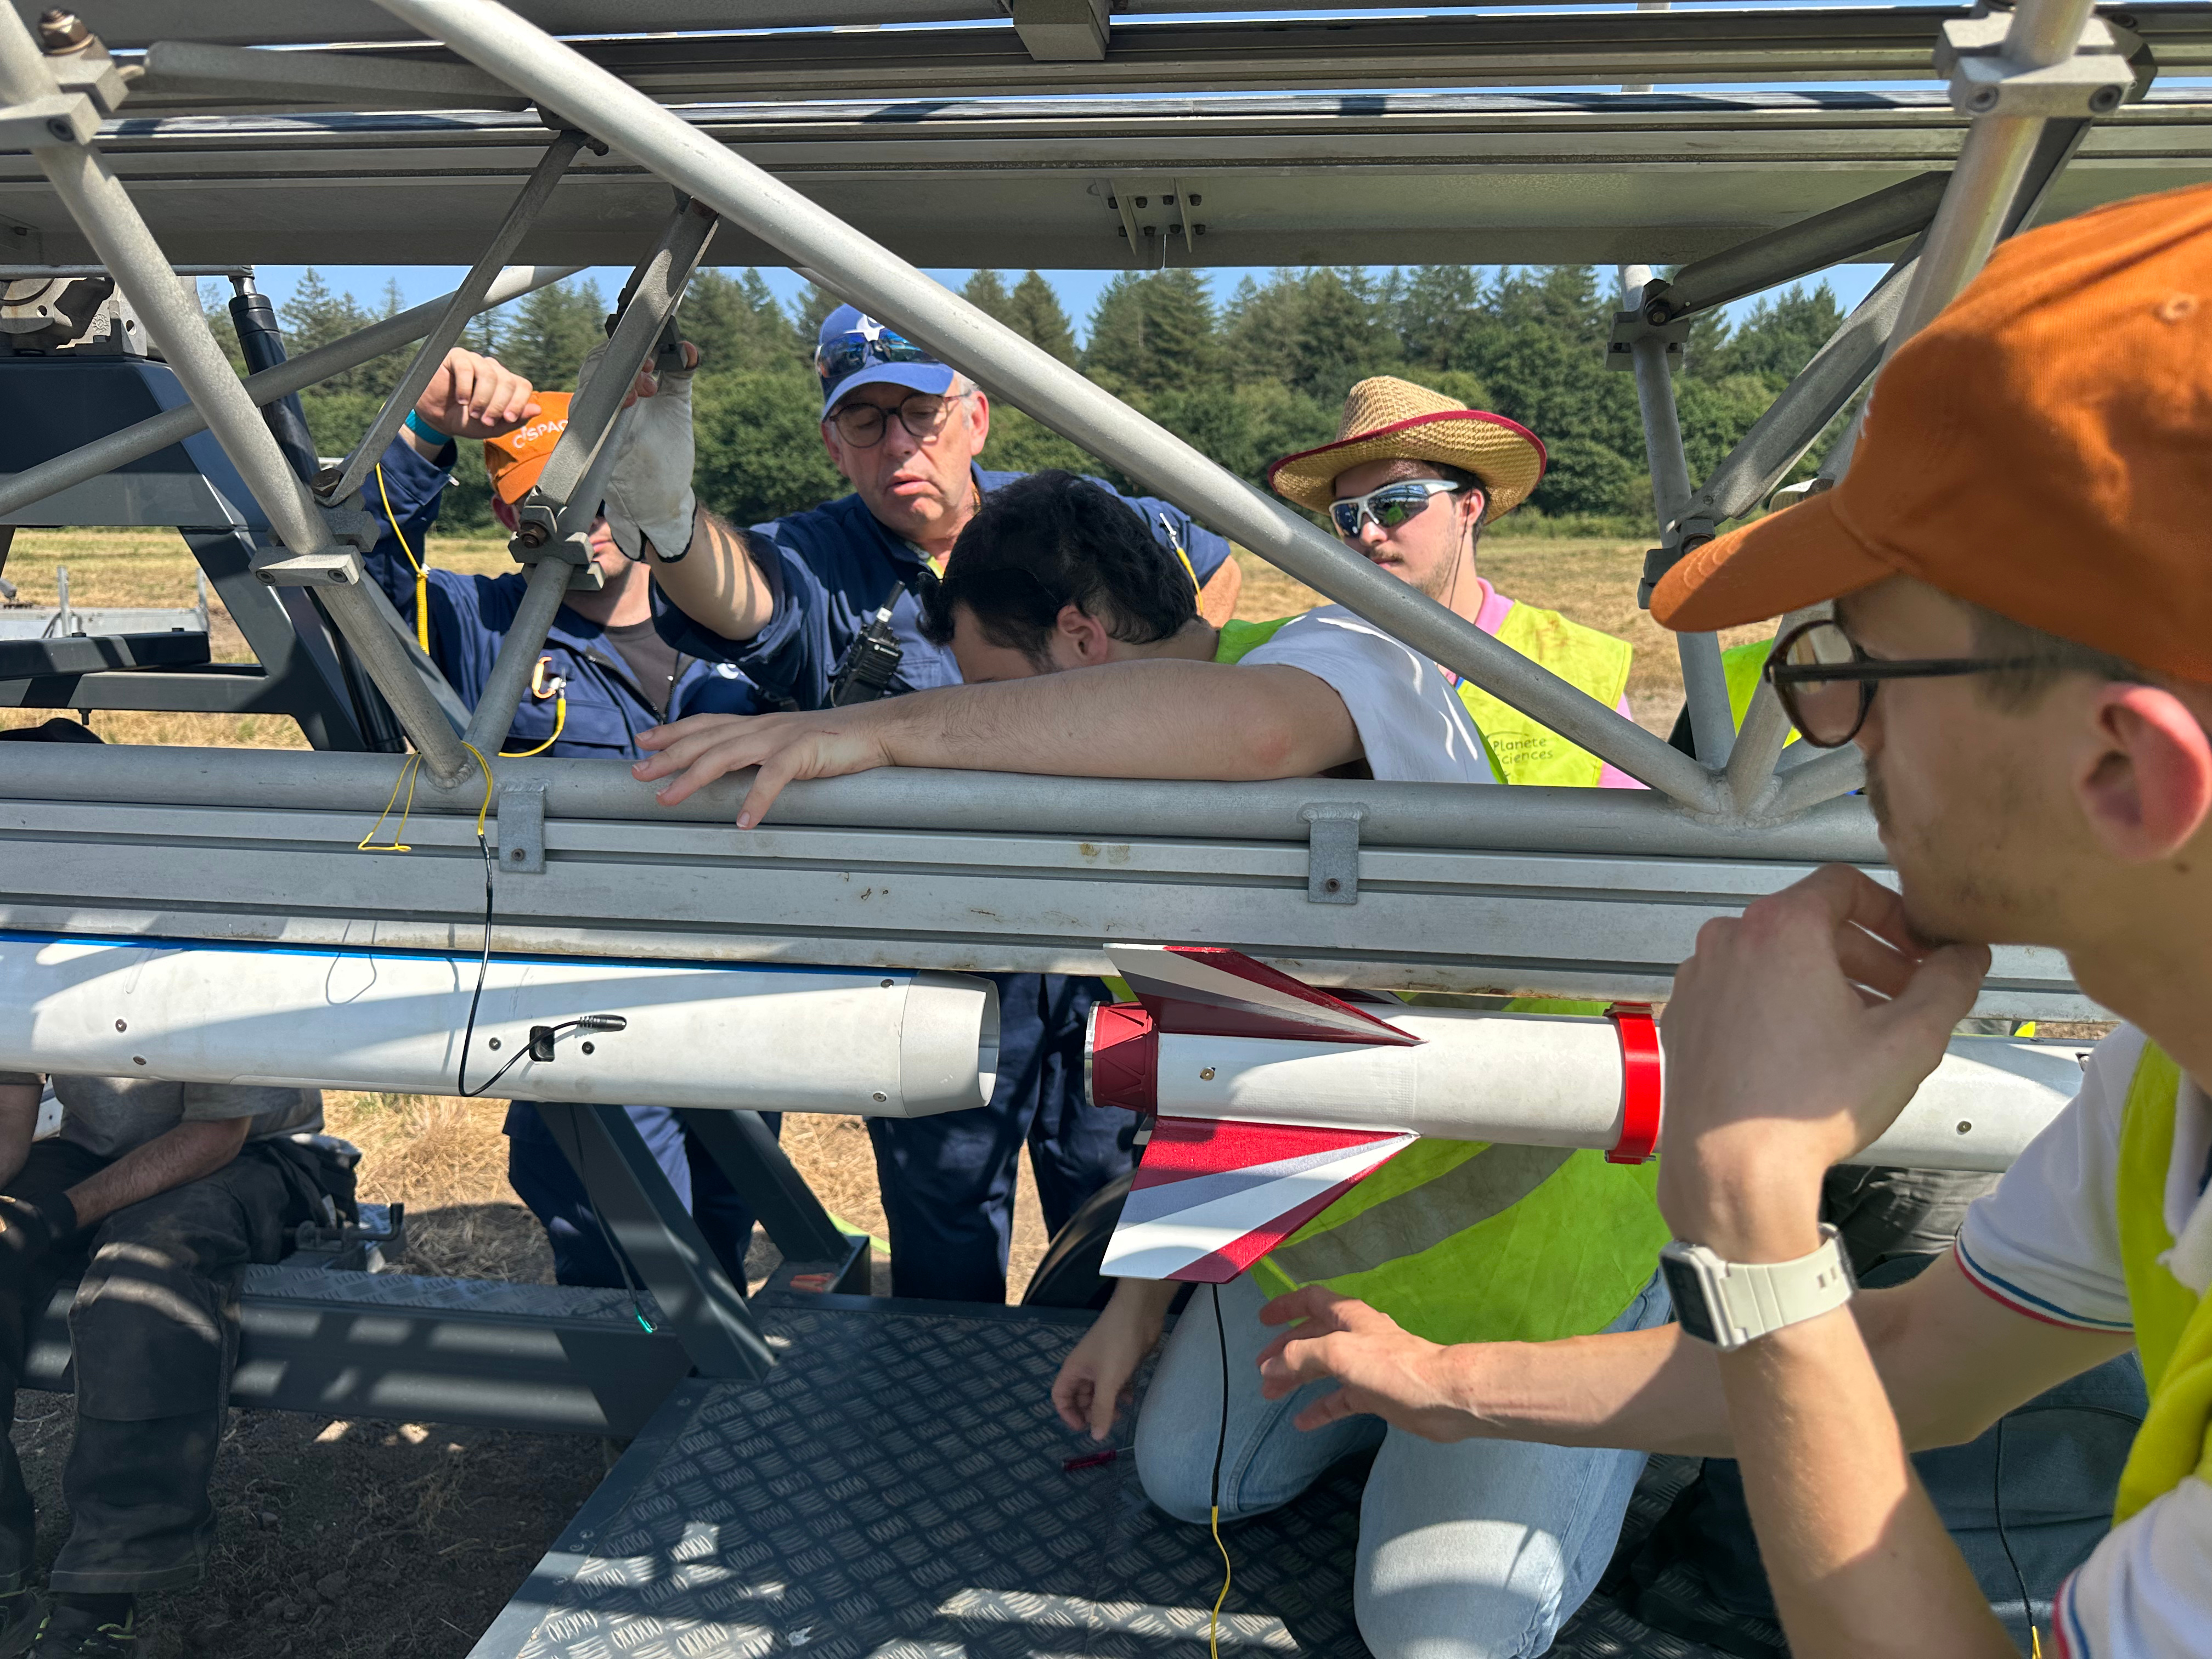
\includegraphics[width=\textwidth]{figures/sp02_mise_rampe.png}
    \end{subfigure}
    \hfill
    \begin{subfigure}[b]{0.32\textwidth}
        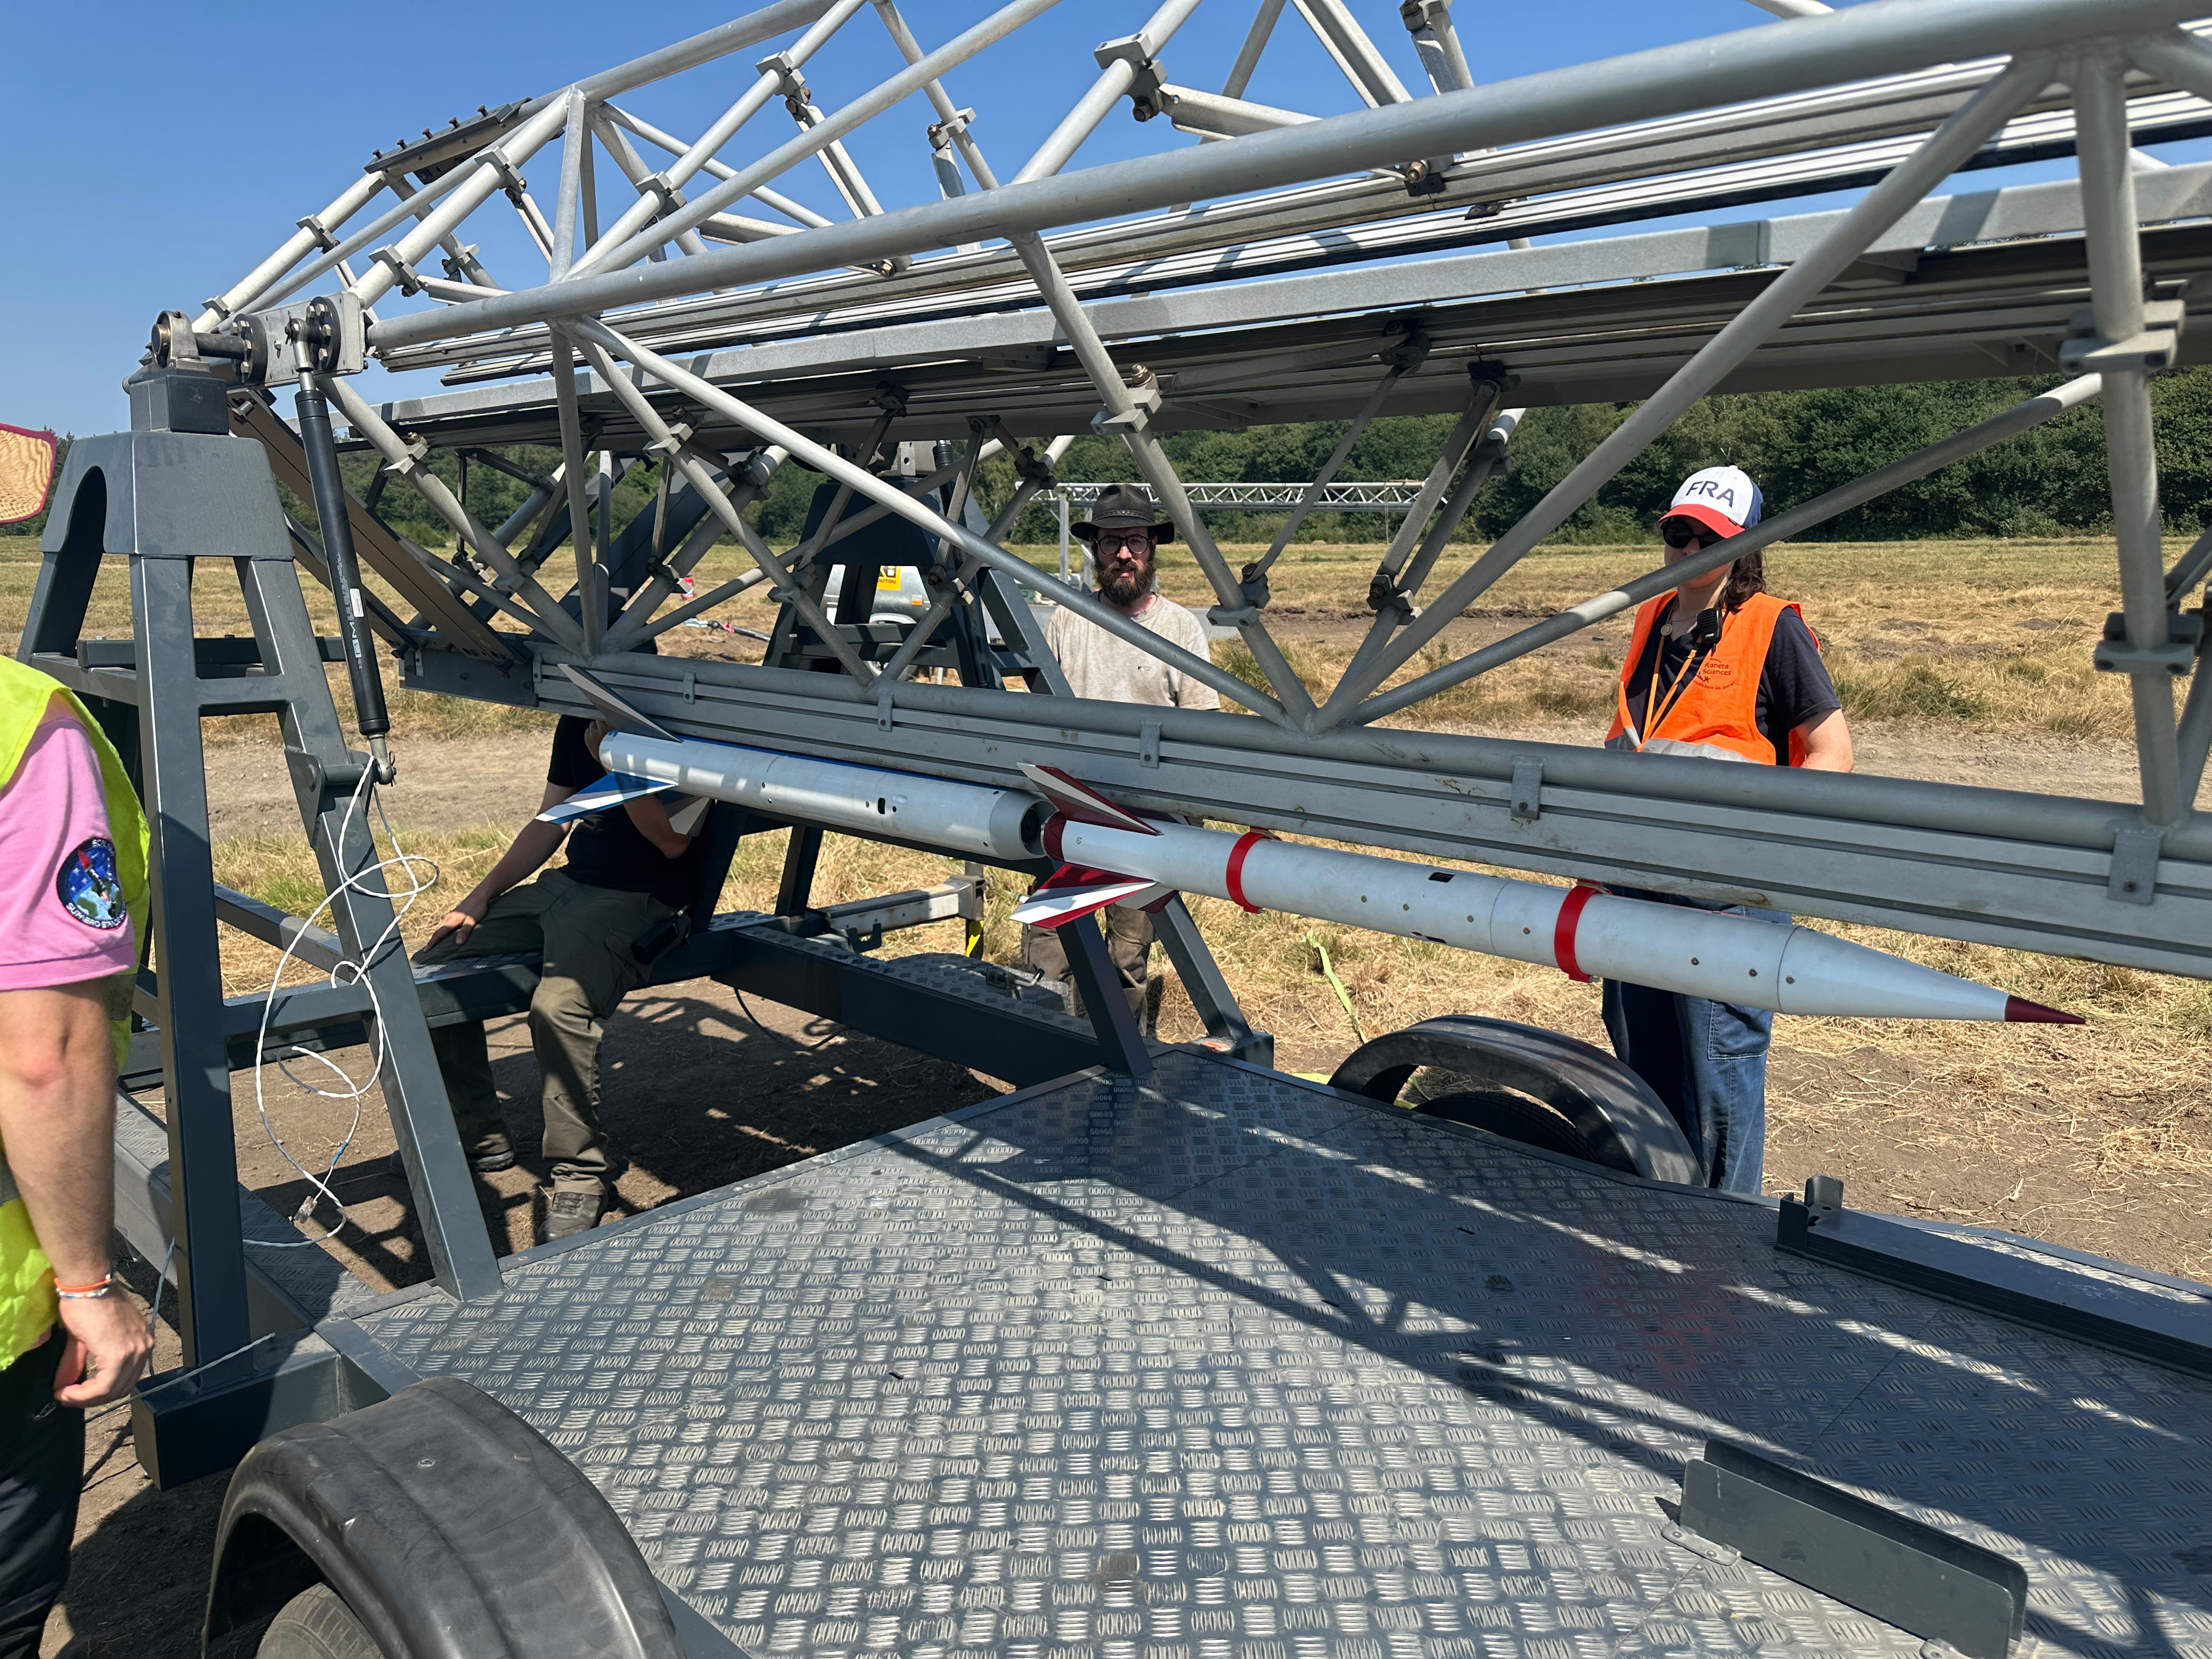
\includegraphics[width=\textwidth]{figures/sp02_mise_rampe1.png}
    \end{subfigure}
    \hfill
    \begin{subfigure}[b]{0.32\textwidth}
        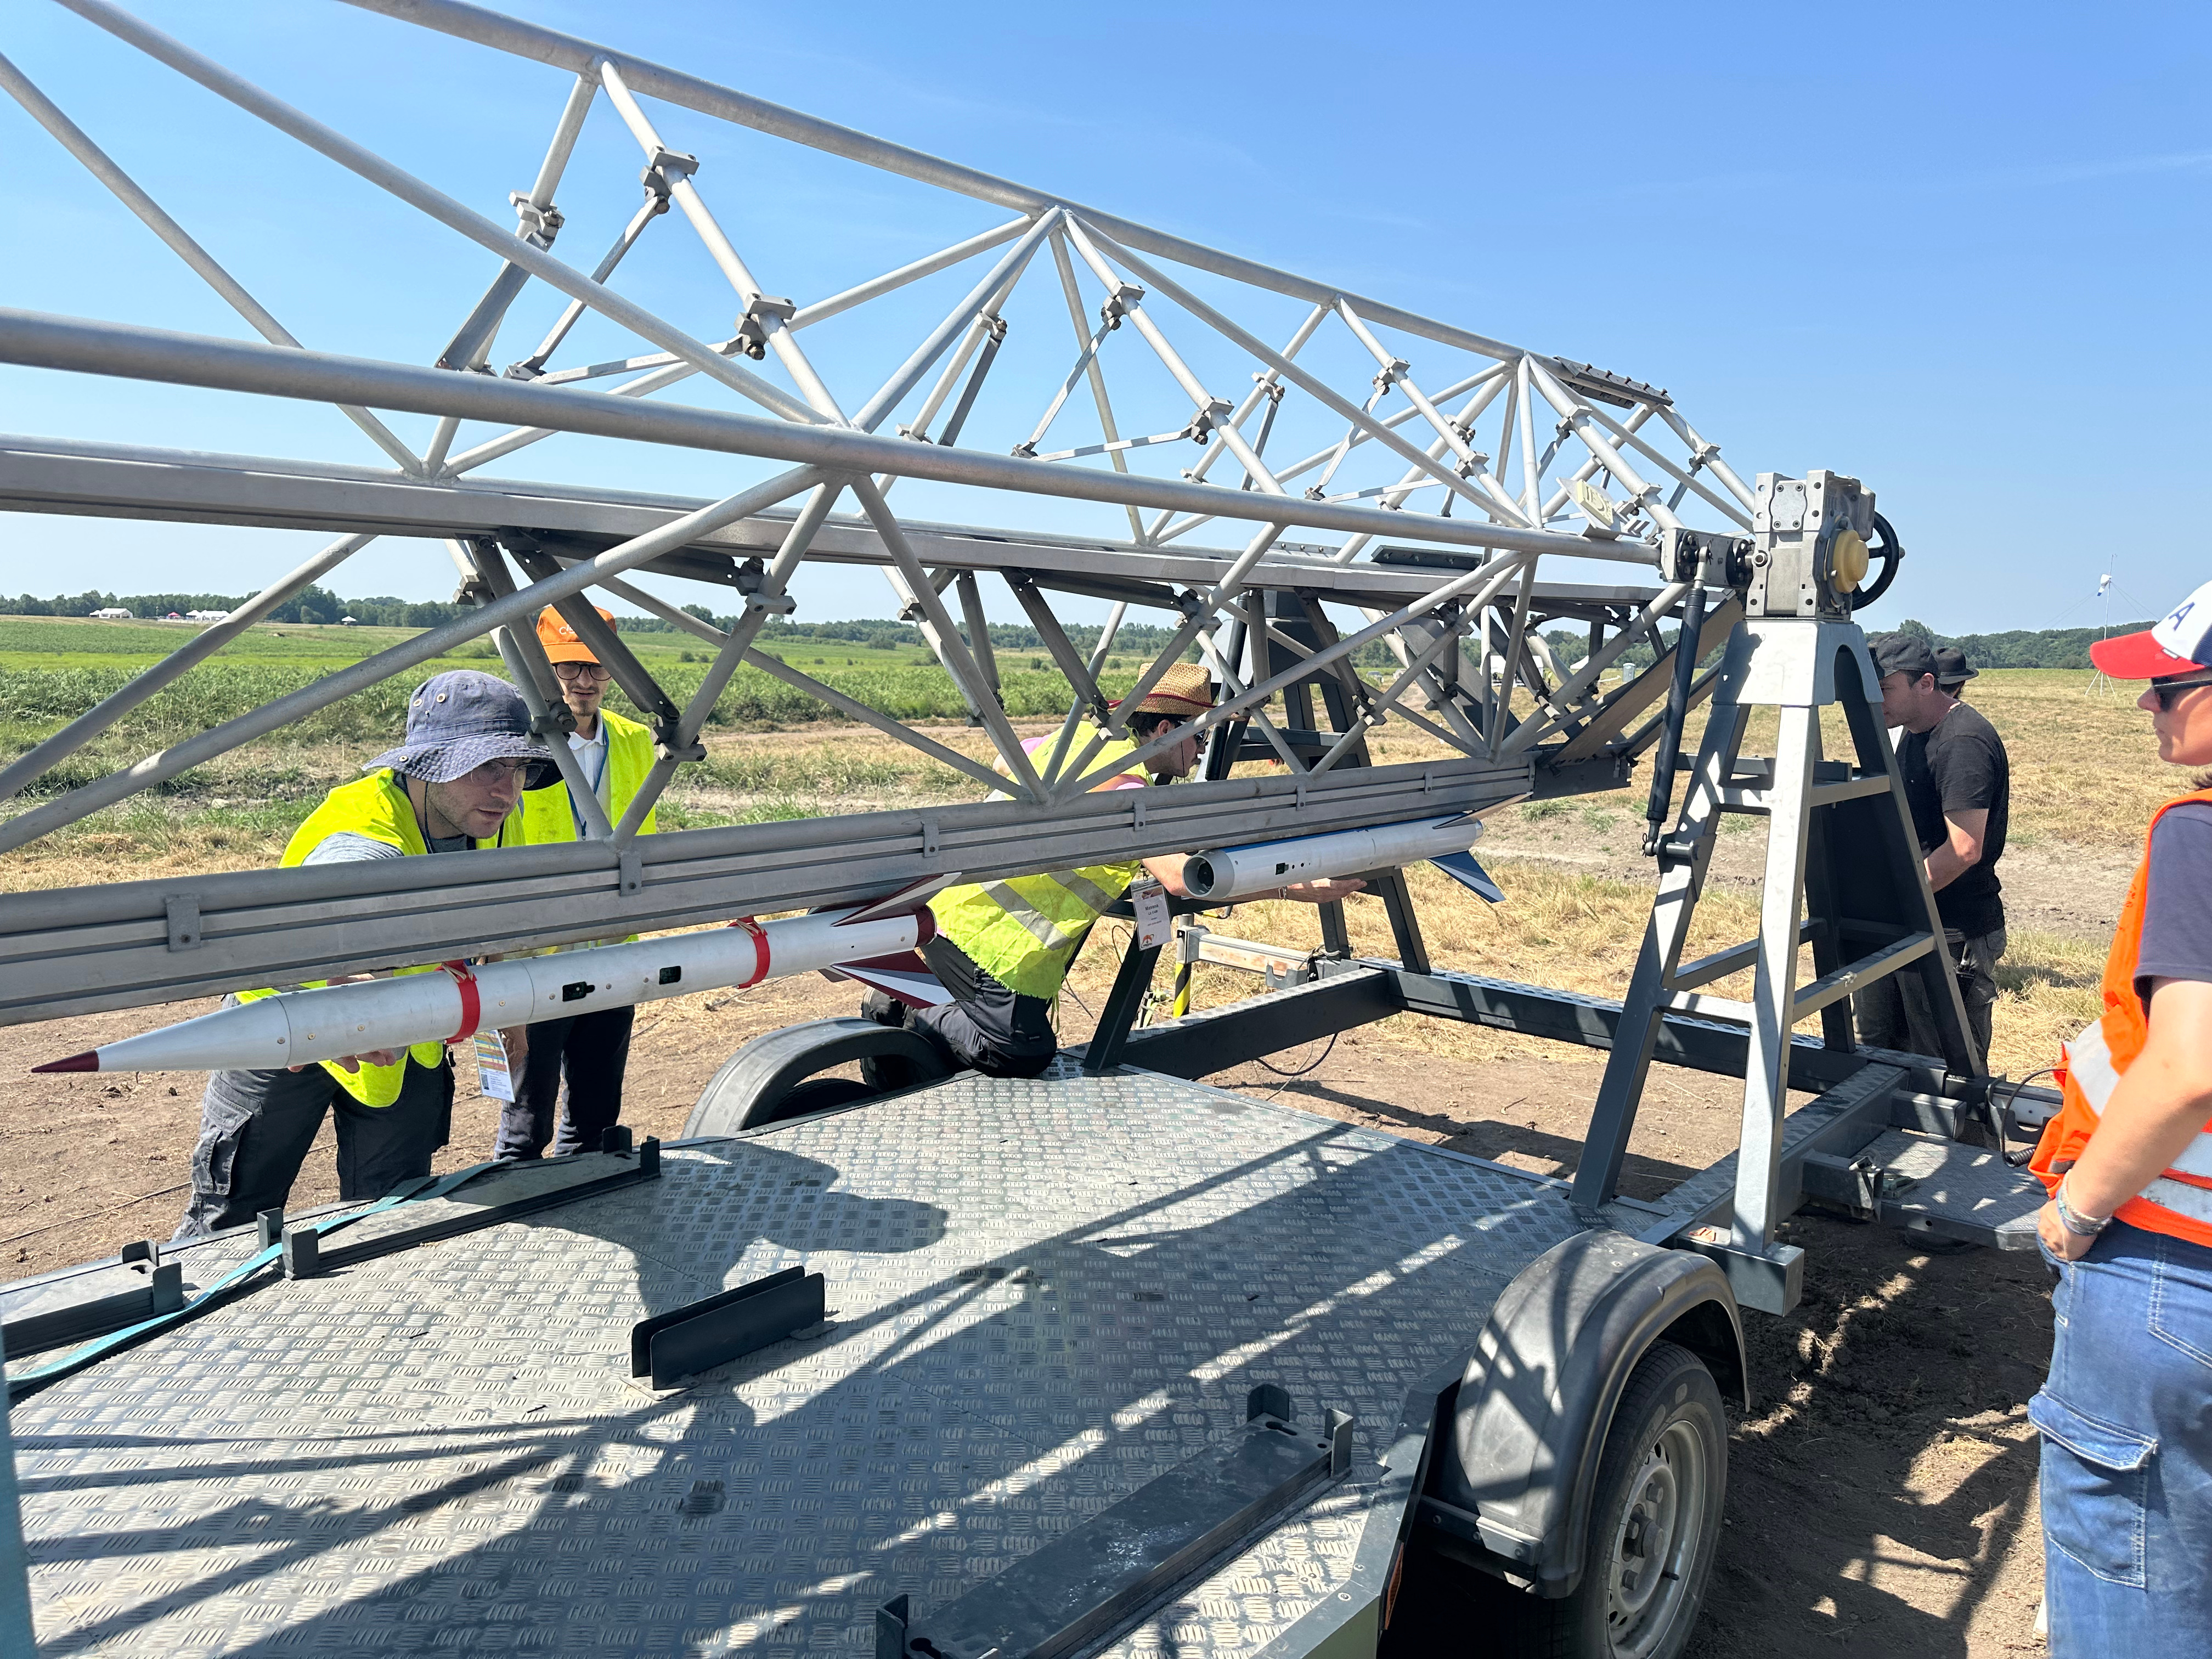
\includegraphics[width=\textwidth]{figures/sp02_mise_rampe3.png}
    \end{subfigure}
    \caption{Compatibilité rampe}
    \label{fig:controle_j2.2}
\end{figure}


\subsubsection{Mercredi : contrôles et défis techniques}
Les nombreux contrôles se sont poursuivis. Grâce à l'intervention de Nathan Garnier, l'allumeur du deuxième étage a pu 
être validé électriquement. Cependant, en fin de journée, malgré les efforts intensifs de Malo et Nathan sur la station 
sol, le code expérience n'était pas finalisé et la chaîne de télémesure n'avait pas encore été validée.

\begin{figure}[!ht]
    \centering
    \begin{subfigure}[b]{0.32\textwidth}
        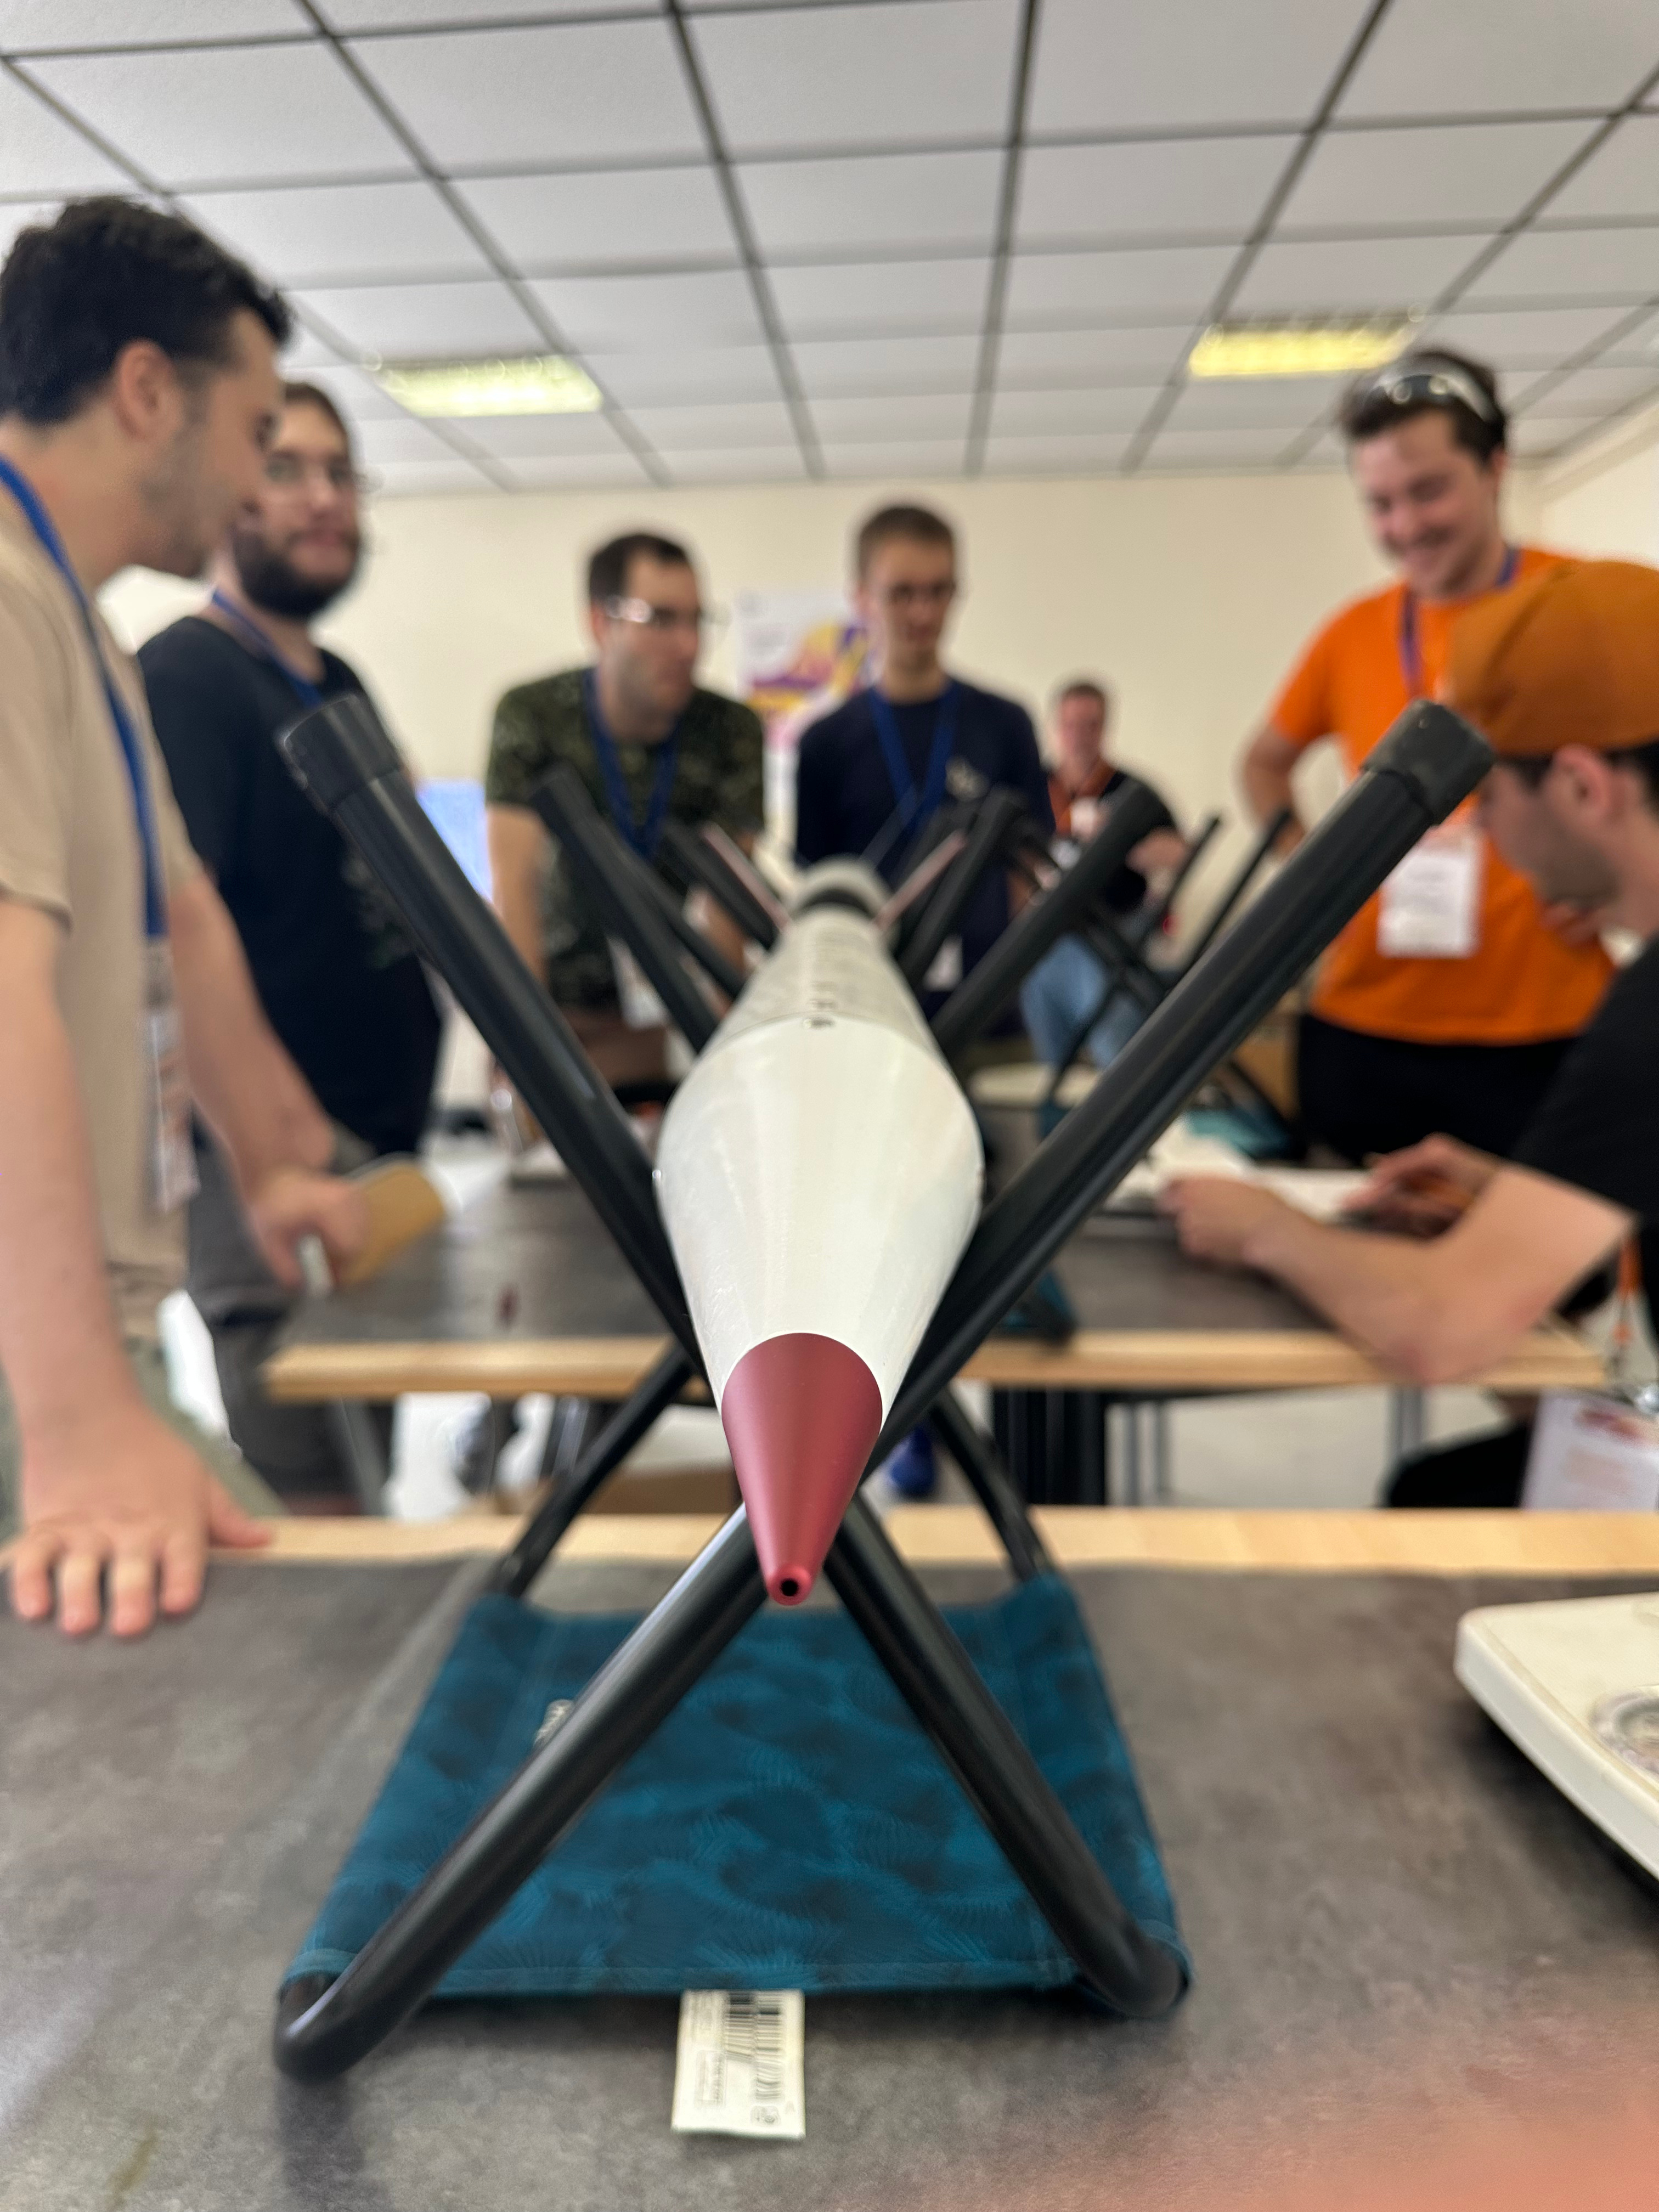
\includegraphics[width=\textwidth]{figures/sp02_controle9.png}
    \end{subfigure}
    \hfill
    \begin{subfigure}[b]{0.32\textwidth}
        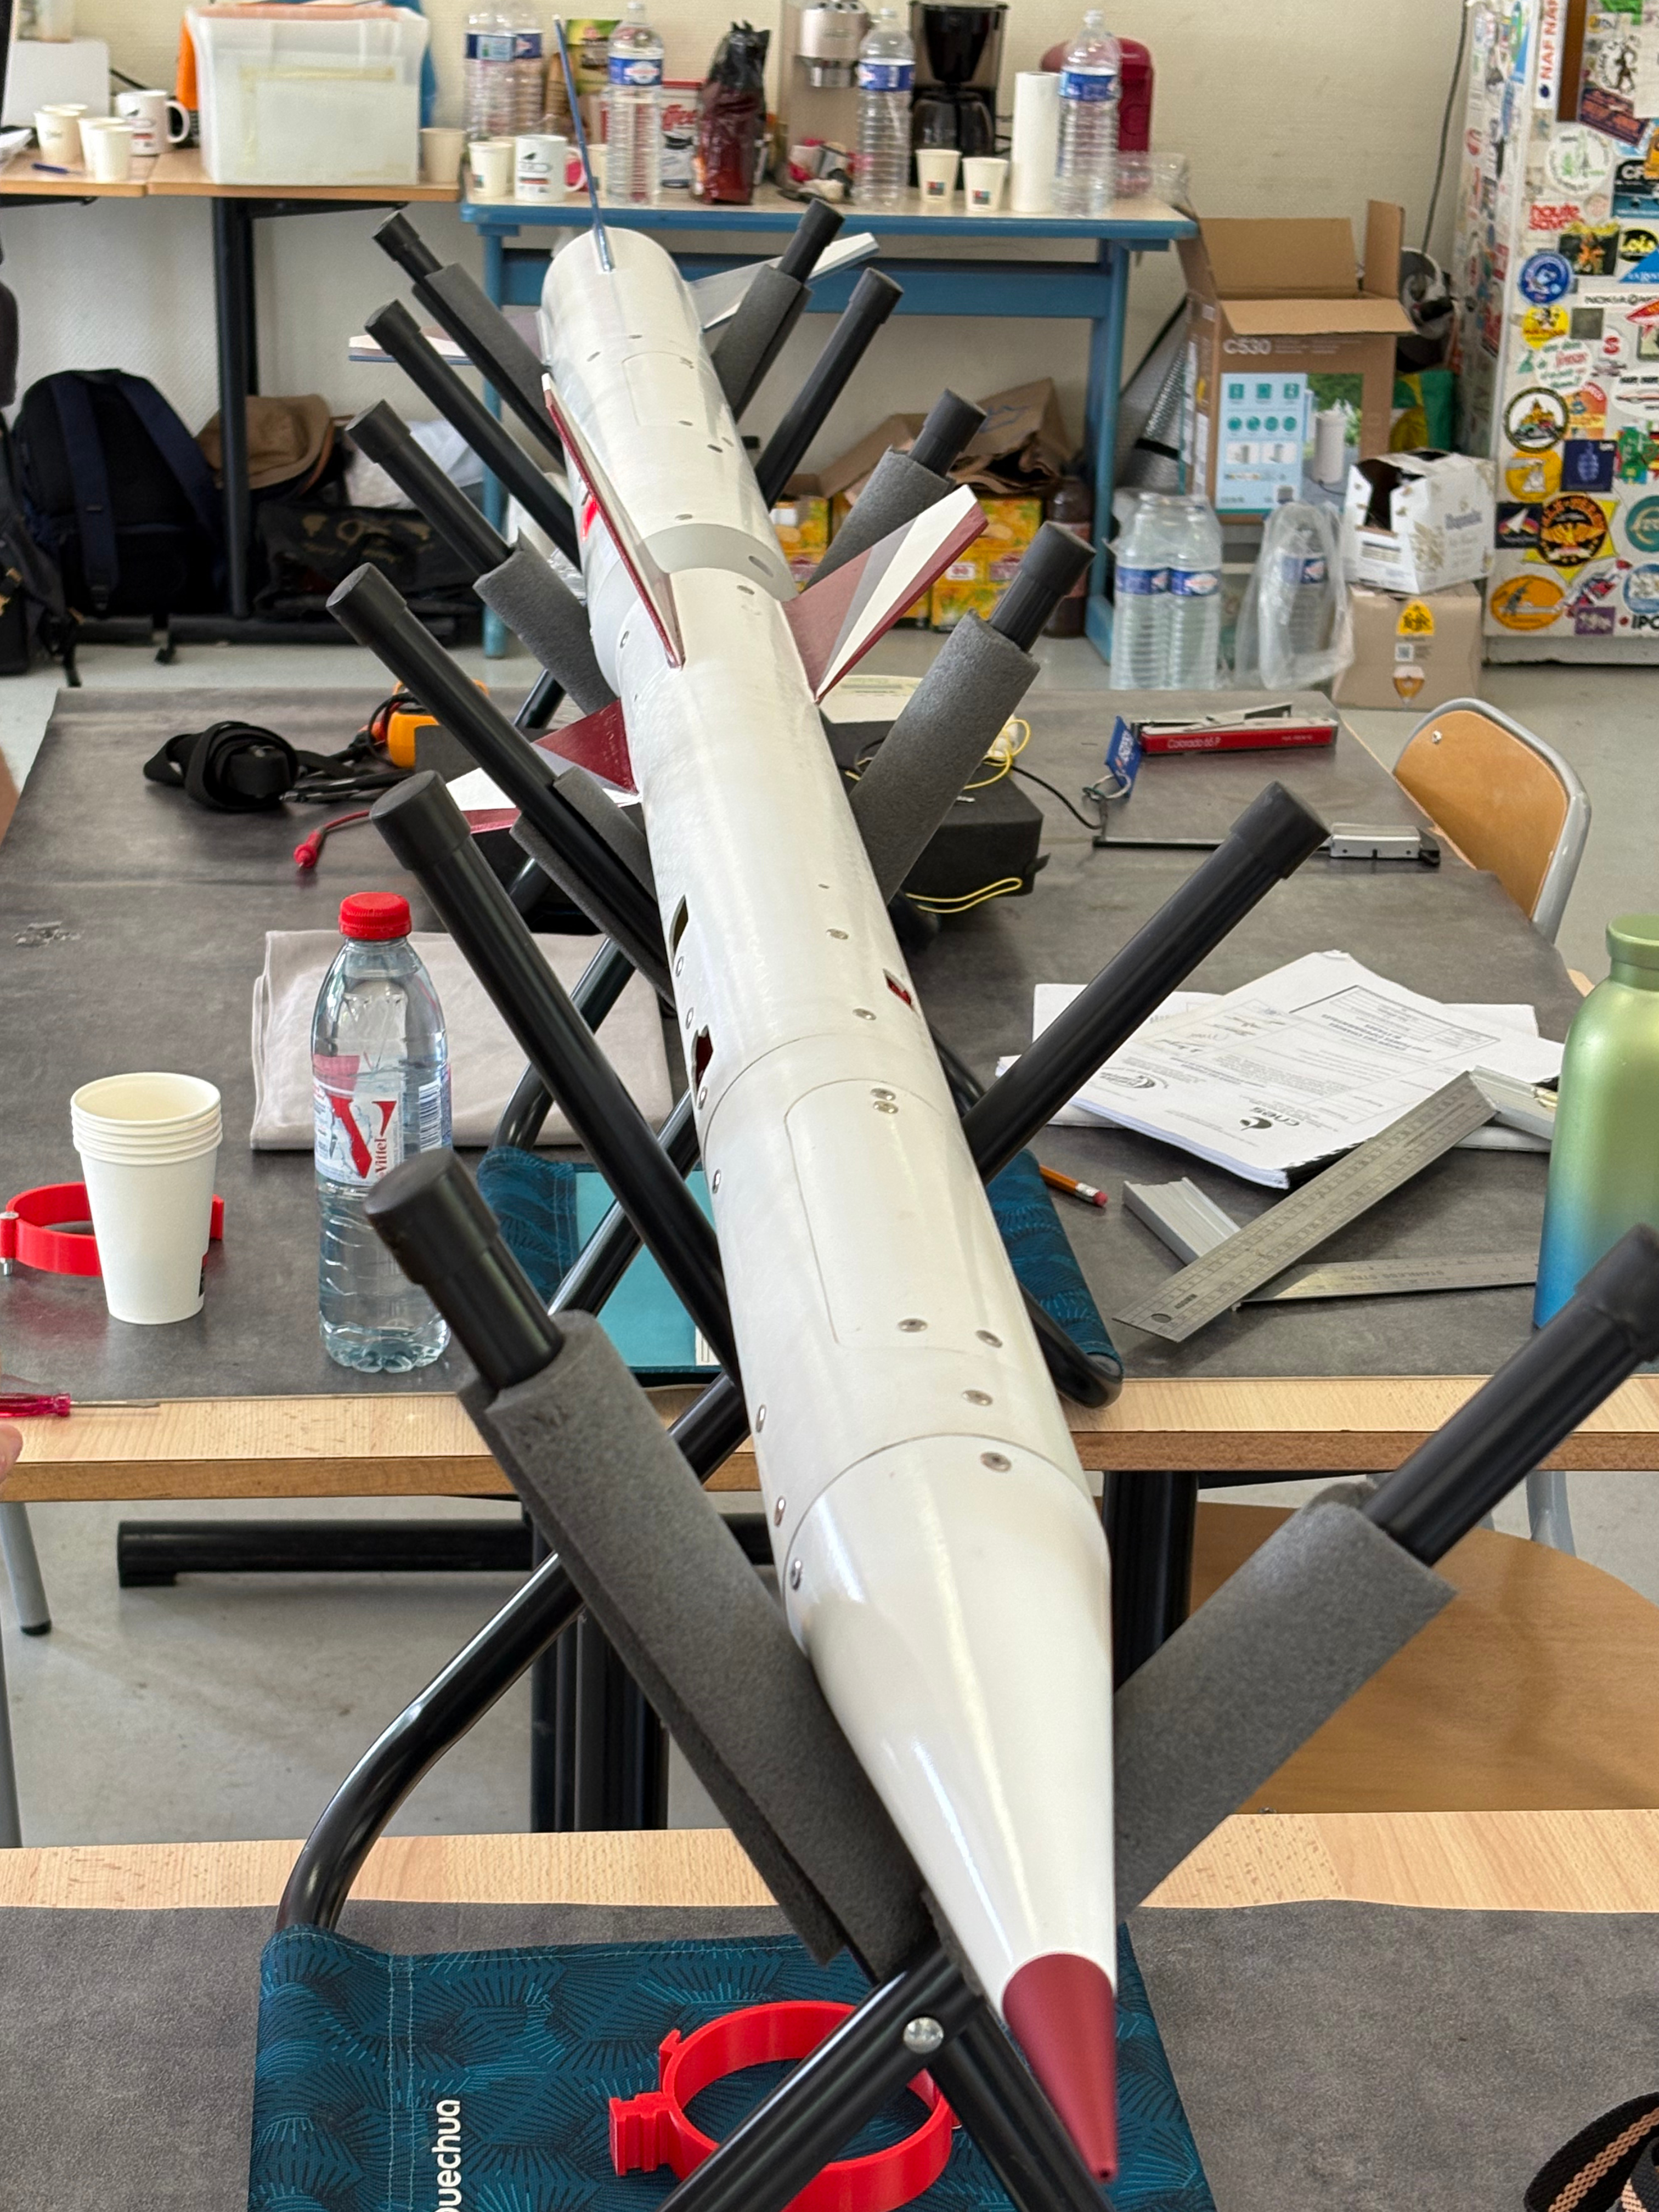
\includegraphics[width=\textwidth]{figures/sp02_controle11.png}
    \end{subfigure}
    \hfill
    \begin{subfigure}[b]{0.32\textwidth}
        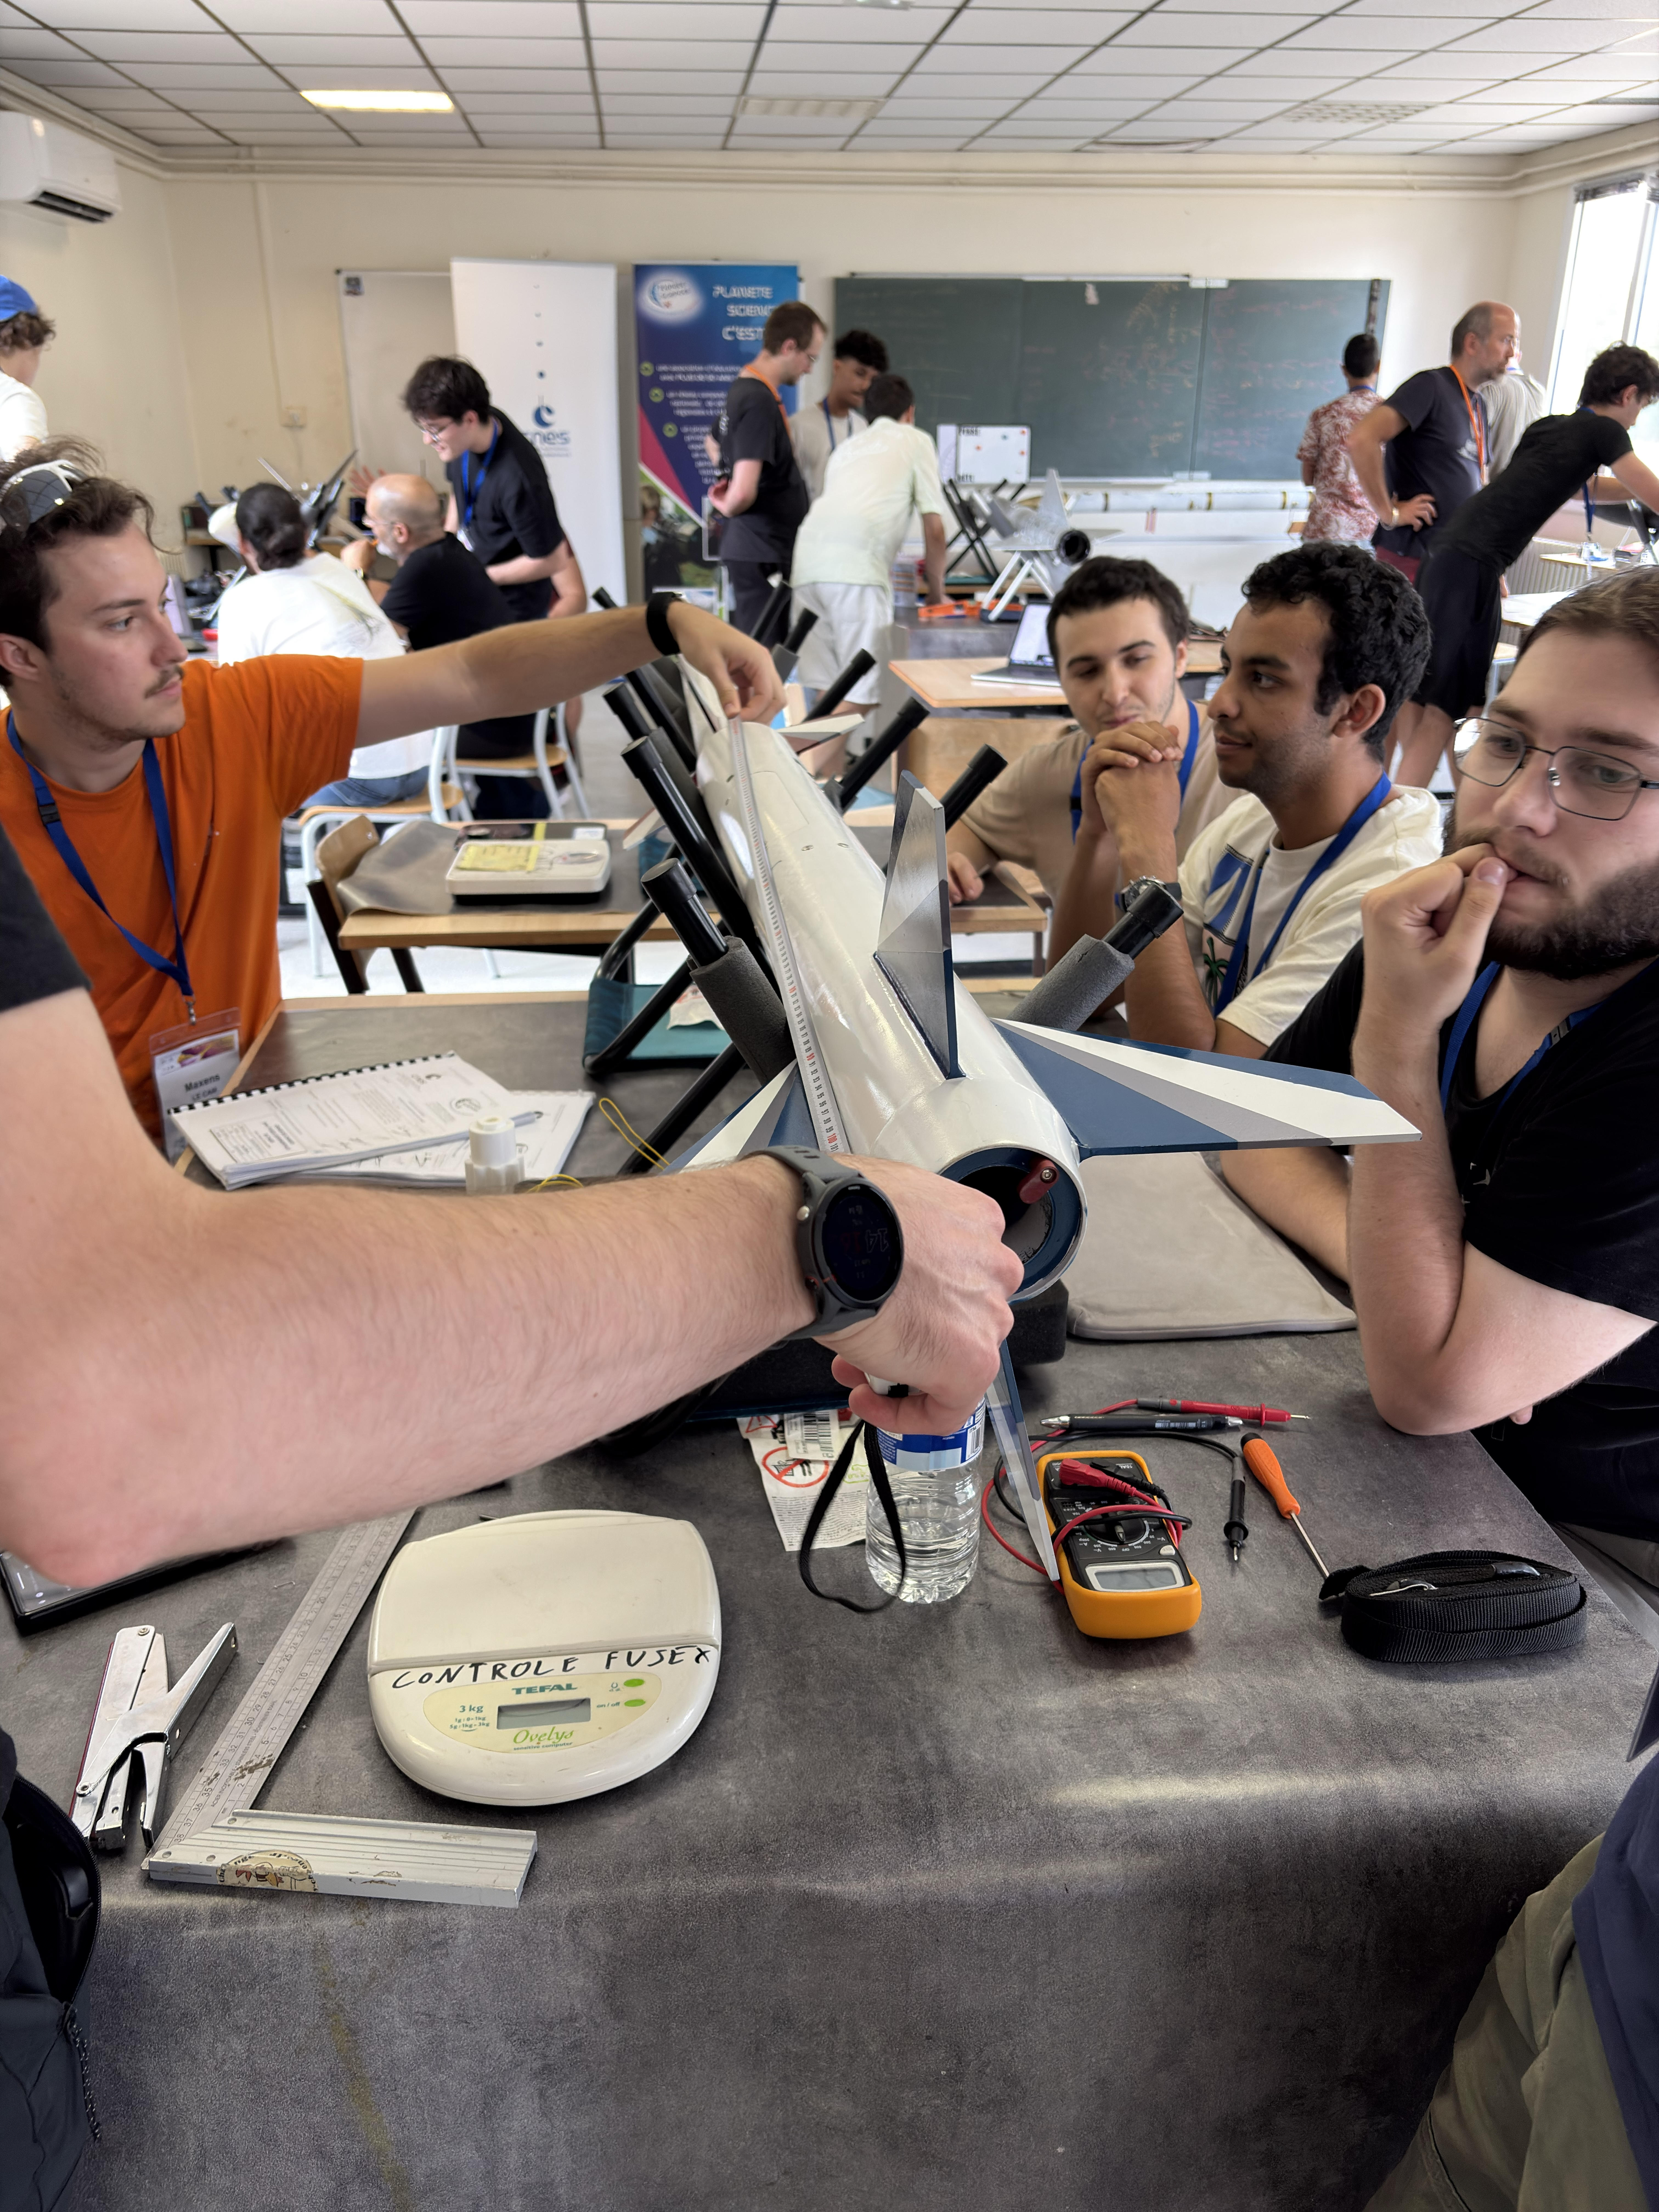
\includegraphics[width=\textwidth]{figures/sp02_controle37.jpg}
    \end{subfigure}
    \caption{Poursuite des contrôles mécaniques}
    \label{fig:controle_j2.2}
\end{figure}



\subsubsection{Jeudi : simplification et qualification}
Face à ces retards, l'équipe a décidé d'abandonner la chaîne de télémesure et de développer un code expérience simplifié. 
Une fois les batteries chargées, la fusée a été remontée en un temps record, avec tous les systèmes branchés. 
Après avoir contrôlé la séquence de lancement et corrigé les derniers bugs, l'équipe était prête pour les vols simulés.

Une chronologie parfaitement exécutée (après quelques ajustements mineurs) et une procédure pyrotechnique maîtrisée par 
Thierry Stillace ont permis de démarrer le vol simulé. Bien que la trappe du premier étage ne se soit pas ouverte lors de la 
première tentative, une seconde chance a été offerte par Flavien et Thierry. Le deuxième vol simulé s'est déroulé sans 
accroc, permettant à l'équipe d'obtenir sa \textbf{qualification}.
\begin{figure}[!ht]
    \centering
    \begin{subfigure}[b]{0.49\textwidth}
        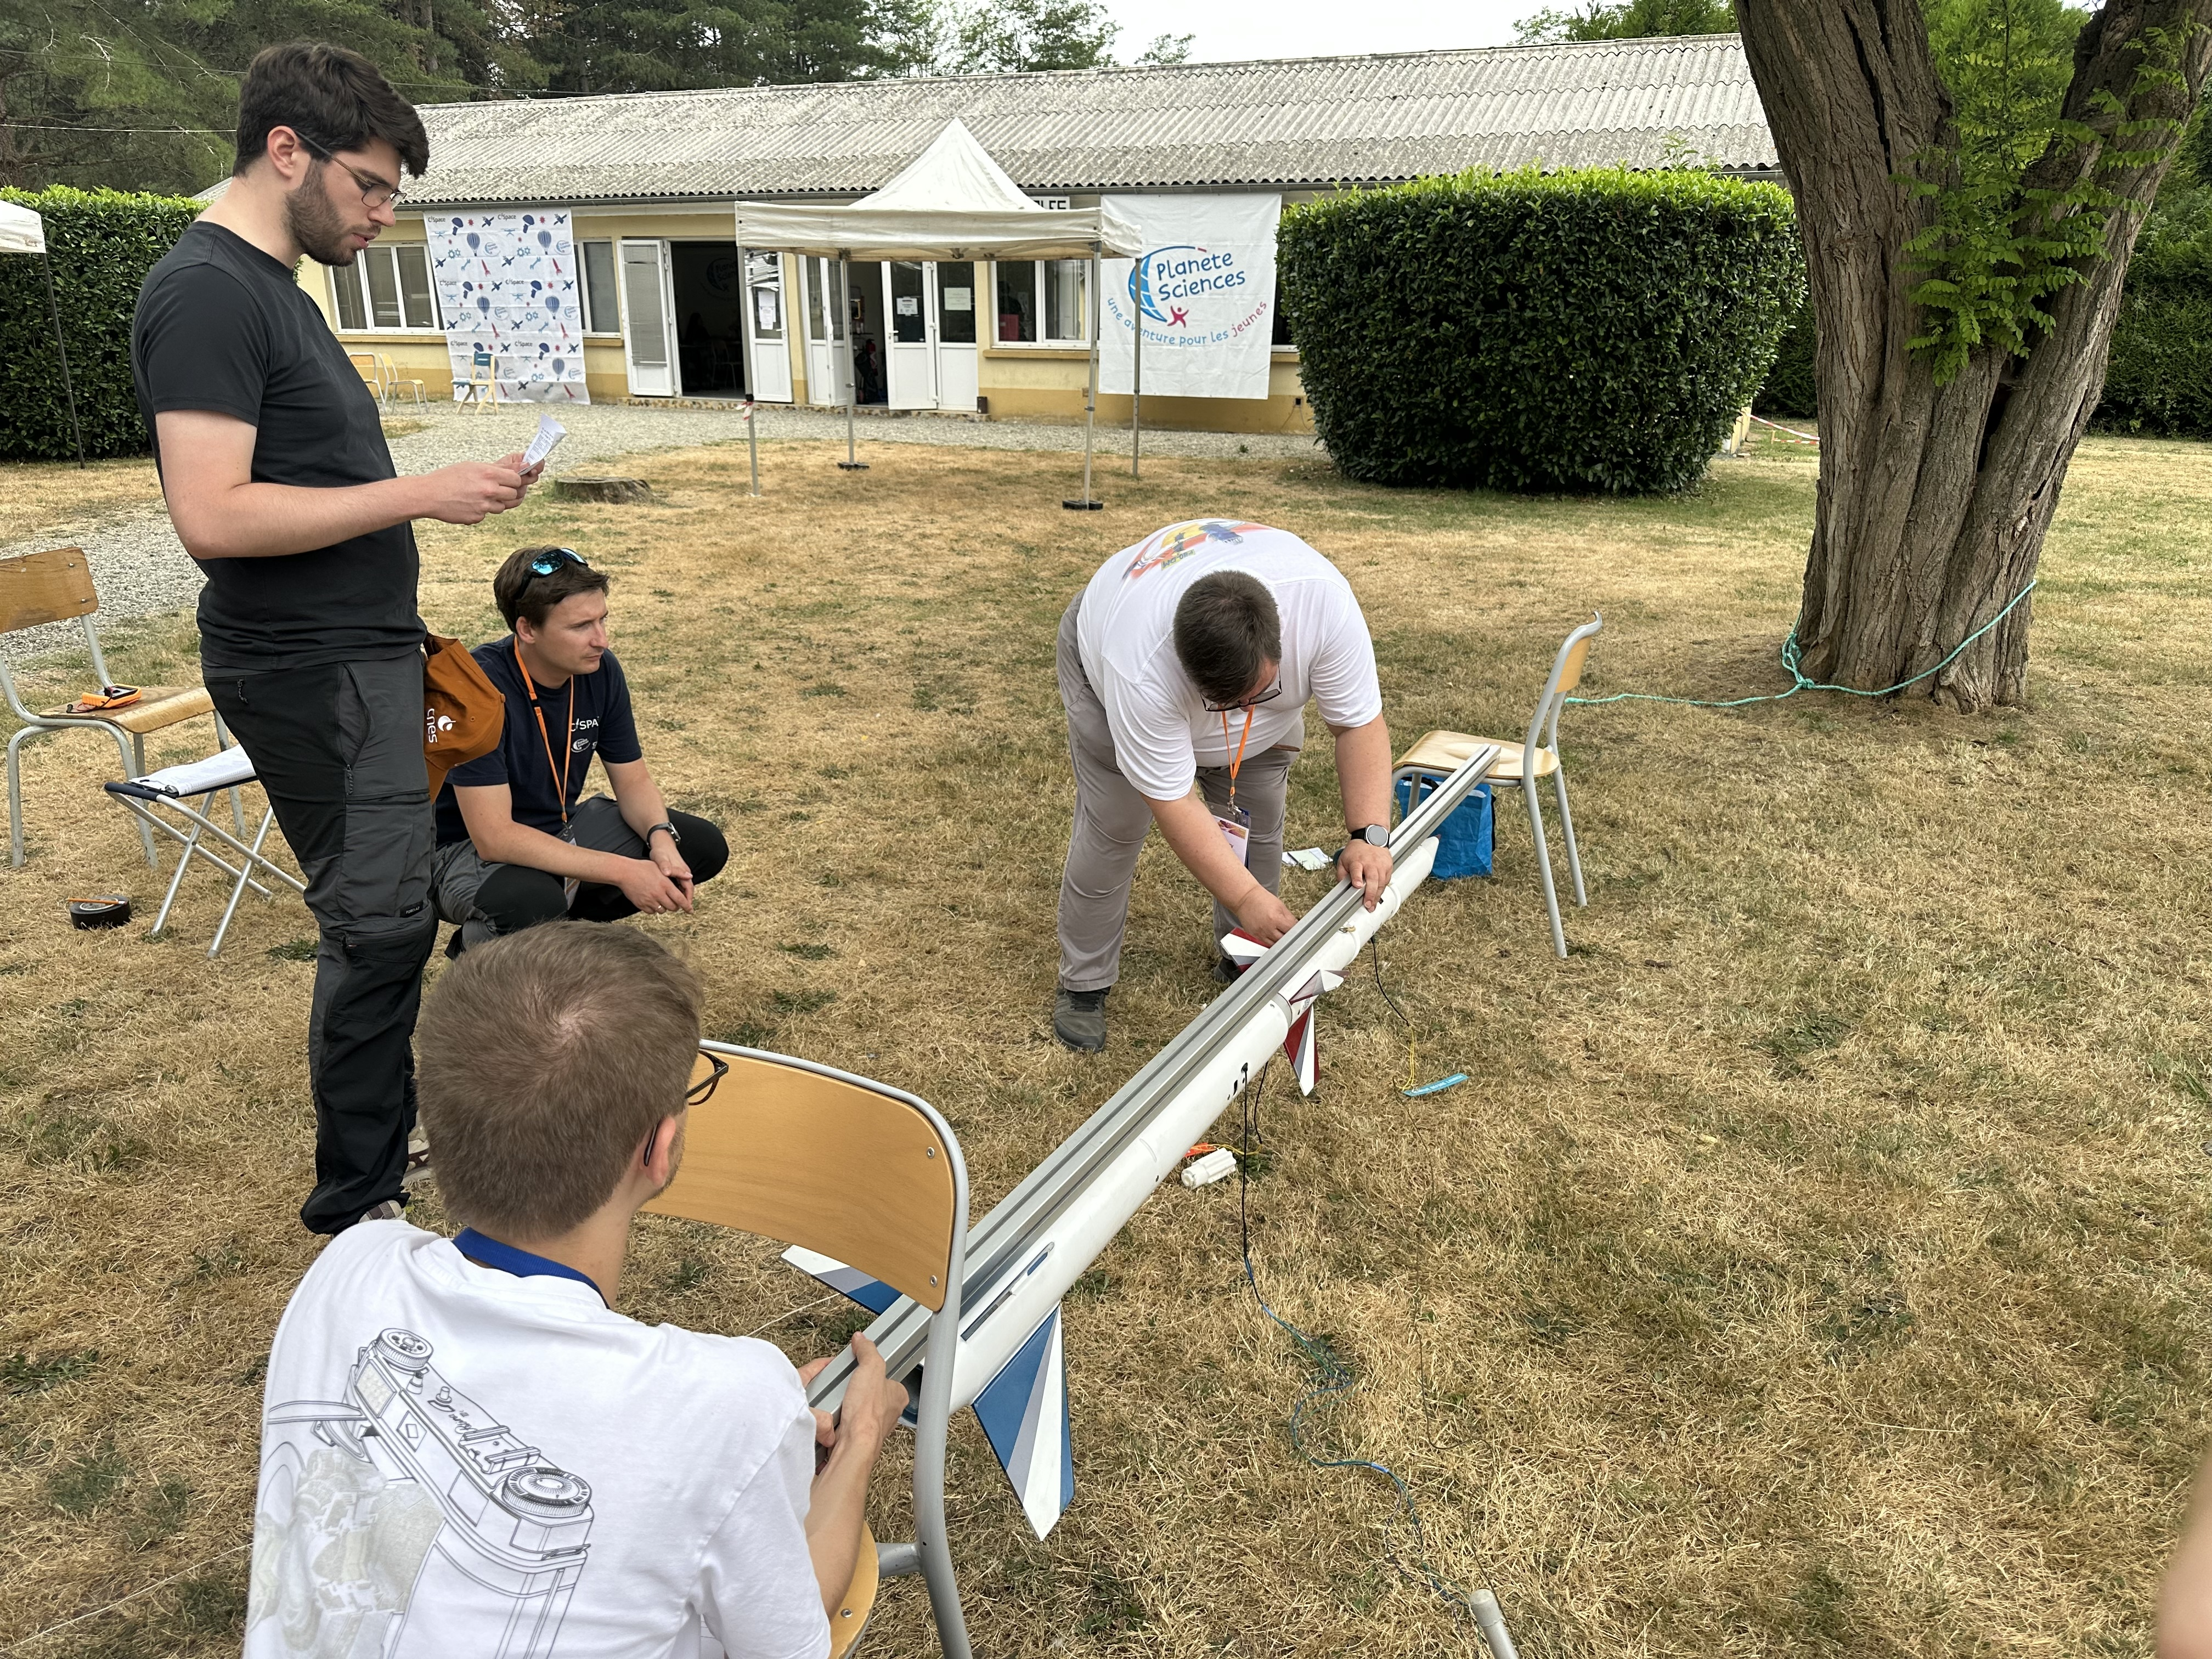
\includegraphics[width=\textwidth]{figures/sp02_controle39.jpg}
    \end{subfigure}
    \hfill
    \begin{subfigure}[b]{0.49\textwidth}
        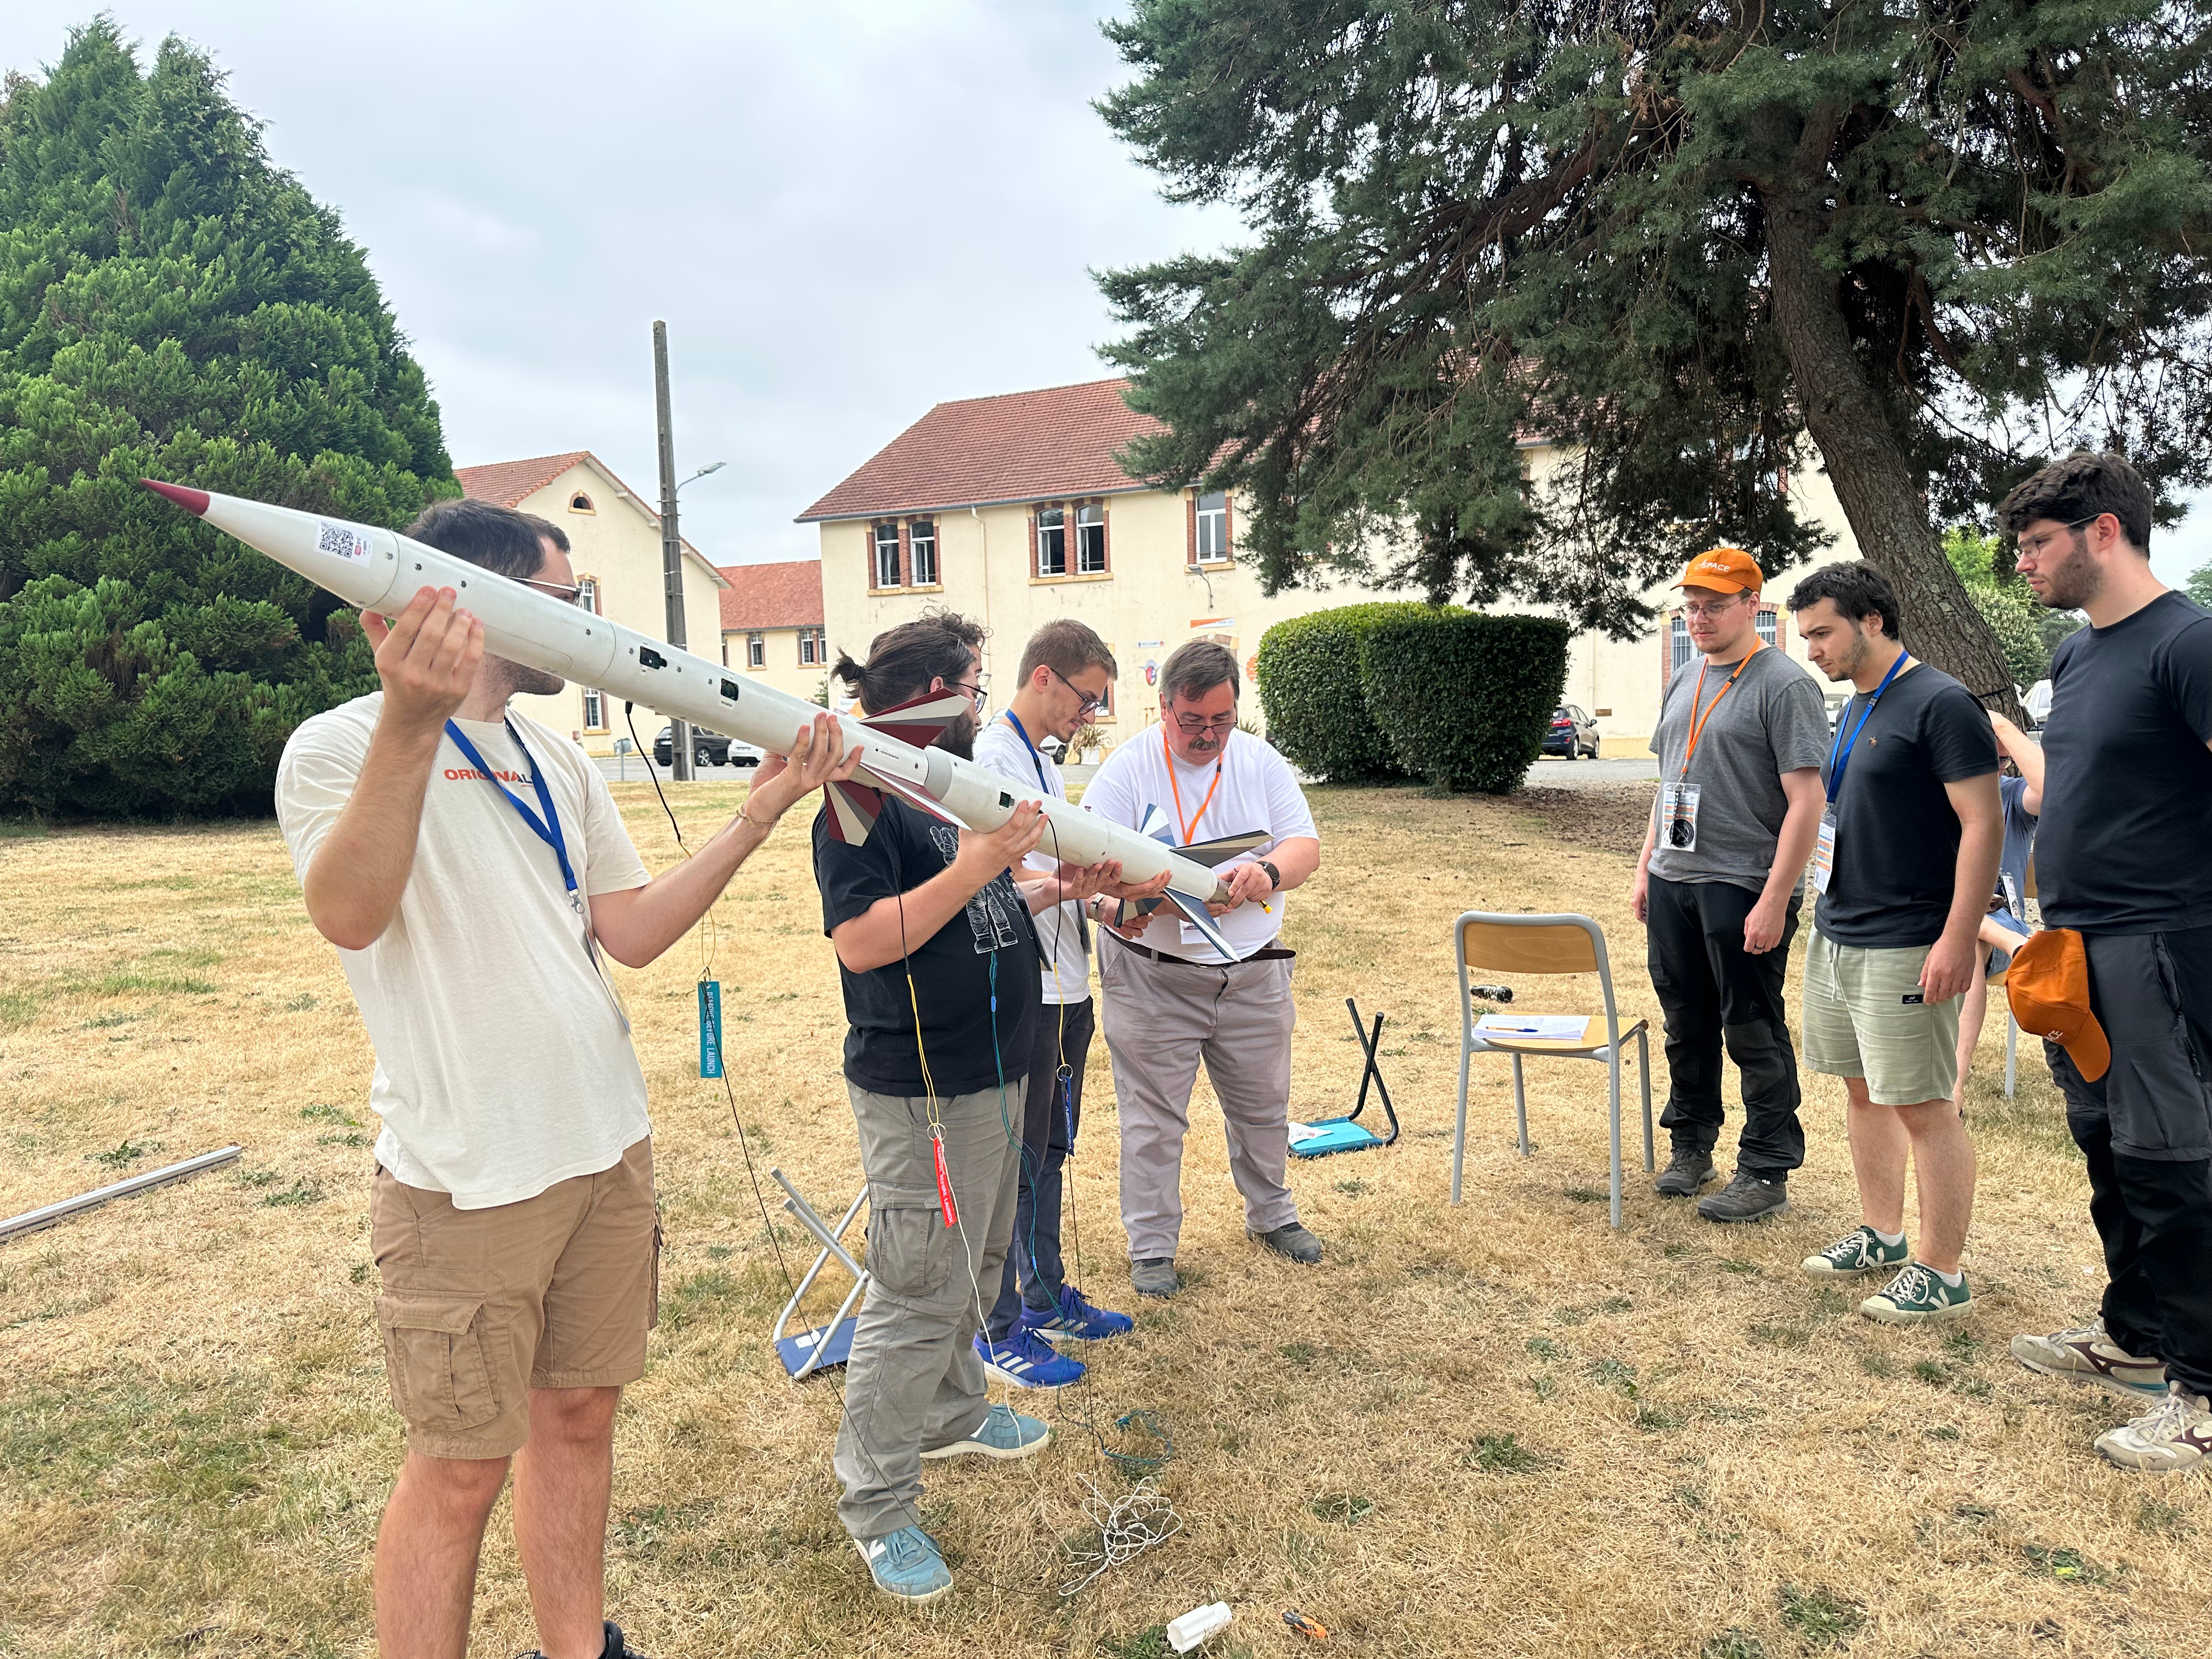
\includegraphics[width=\textwidth]{figures/sp02_controle16.png}
    \end{subfigure}
    \caption{Vol simulé}
    \label{fig:Vol_simule}
\end{figure}


\newpage
\subsubsection{Vendredi : jour de lancement}
Le vendredi matin, la fusée était montée et prête en Zone Air-Sol (ZAS) sous un ciel très nuageux, avec 
un plafond bas. Malgré la pluie lors de la mise en rampe, la chronologie s'est déroulée parfaitement, tant du côté de 
l'équipe que des pyrotechniciens du CNES. Au décollage, après un compte à rebours nominal, les deux étages se sont 
séparés et ont disparu dans les nuages. Après quelques secondes, le bruit d'un parachute s'ouvrant a été entendu, 
suivi d'un bruit aérodynamique de redescente, indiquant un \textit{POC balistique}.

\begin{figure}[H]
    \centering
    % Première ligne : 2 images
    \begin{subfigure}{0.45\textwidth}
        \centering
        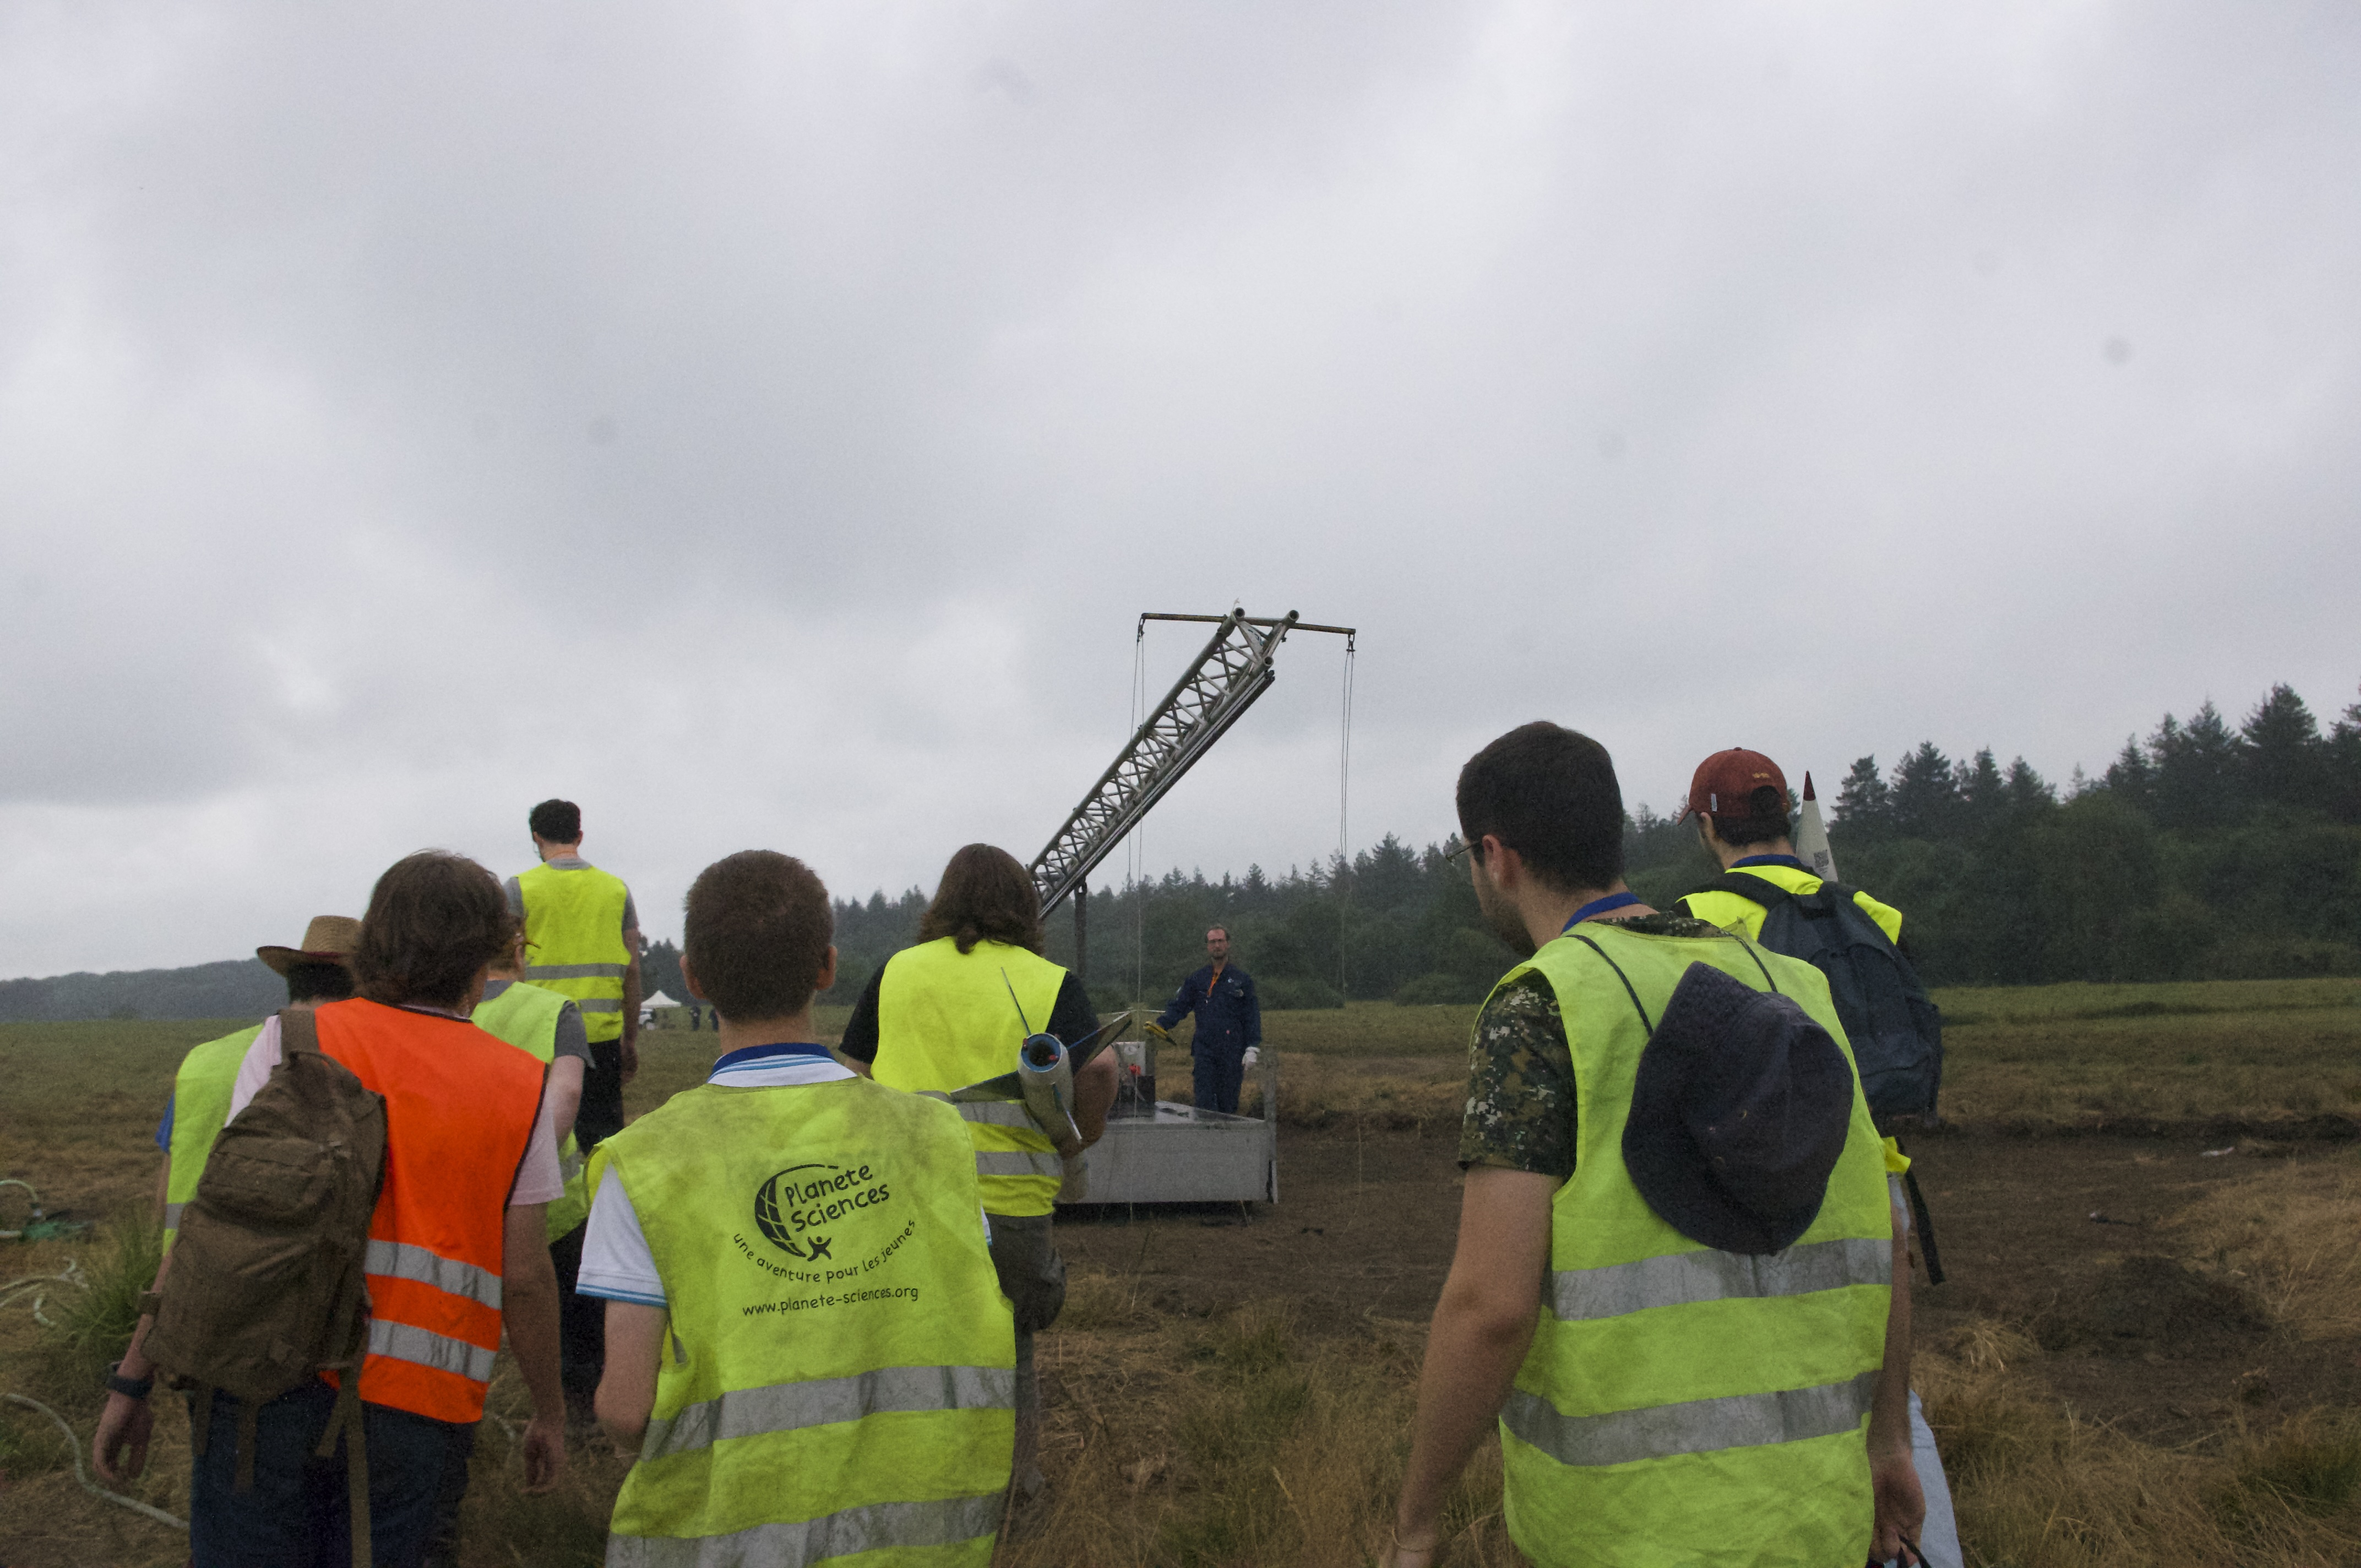
\includegraphics[width=\linewidth]{figures/sp02_lancement8.jpeg}
    \end{subfigure}
    \hfill % Espacement horizontal entre les sous-figures
    \begin{subfigure}{0.45\textwidth}
        \centering
        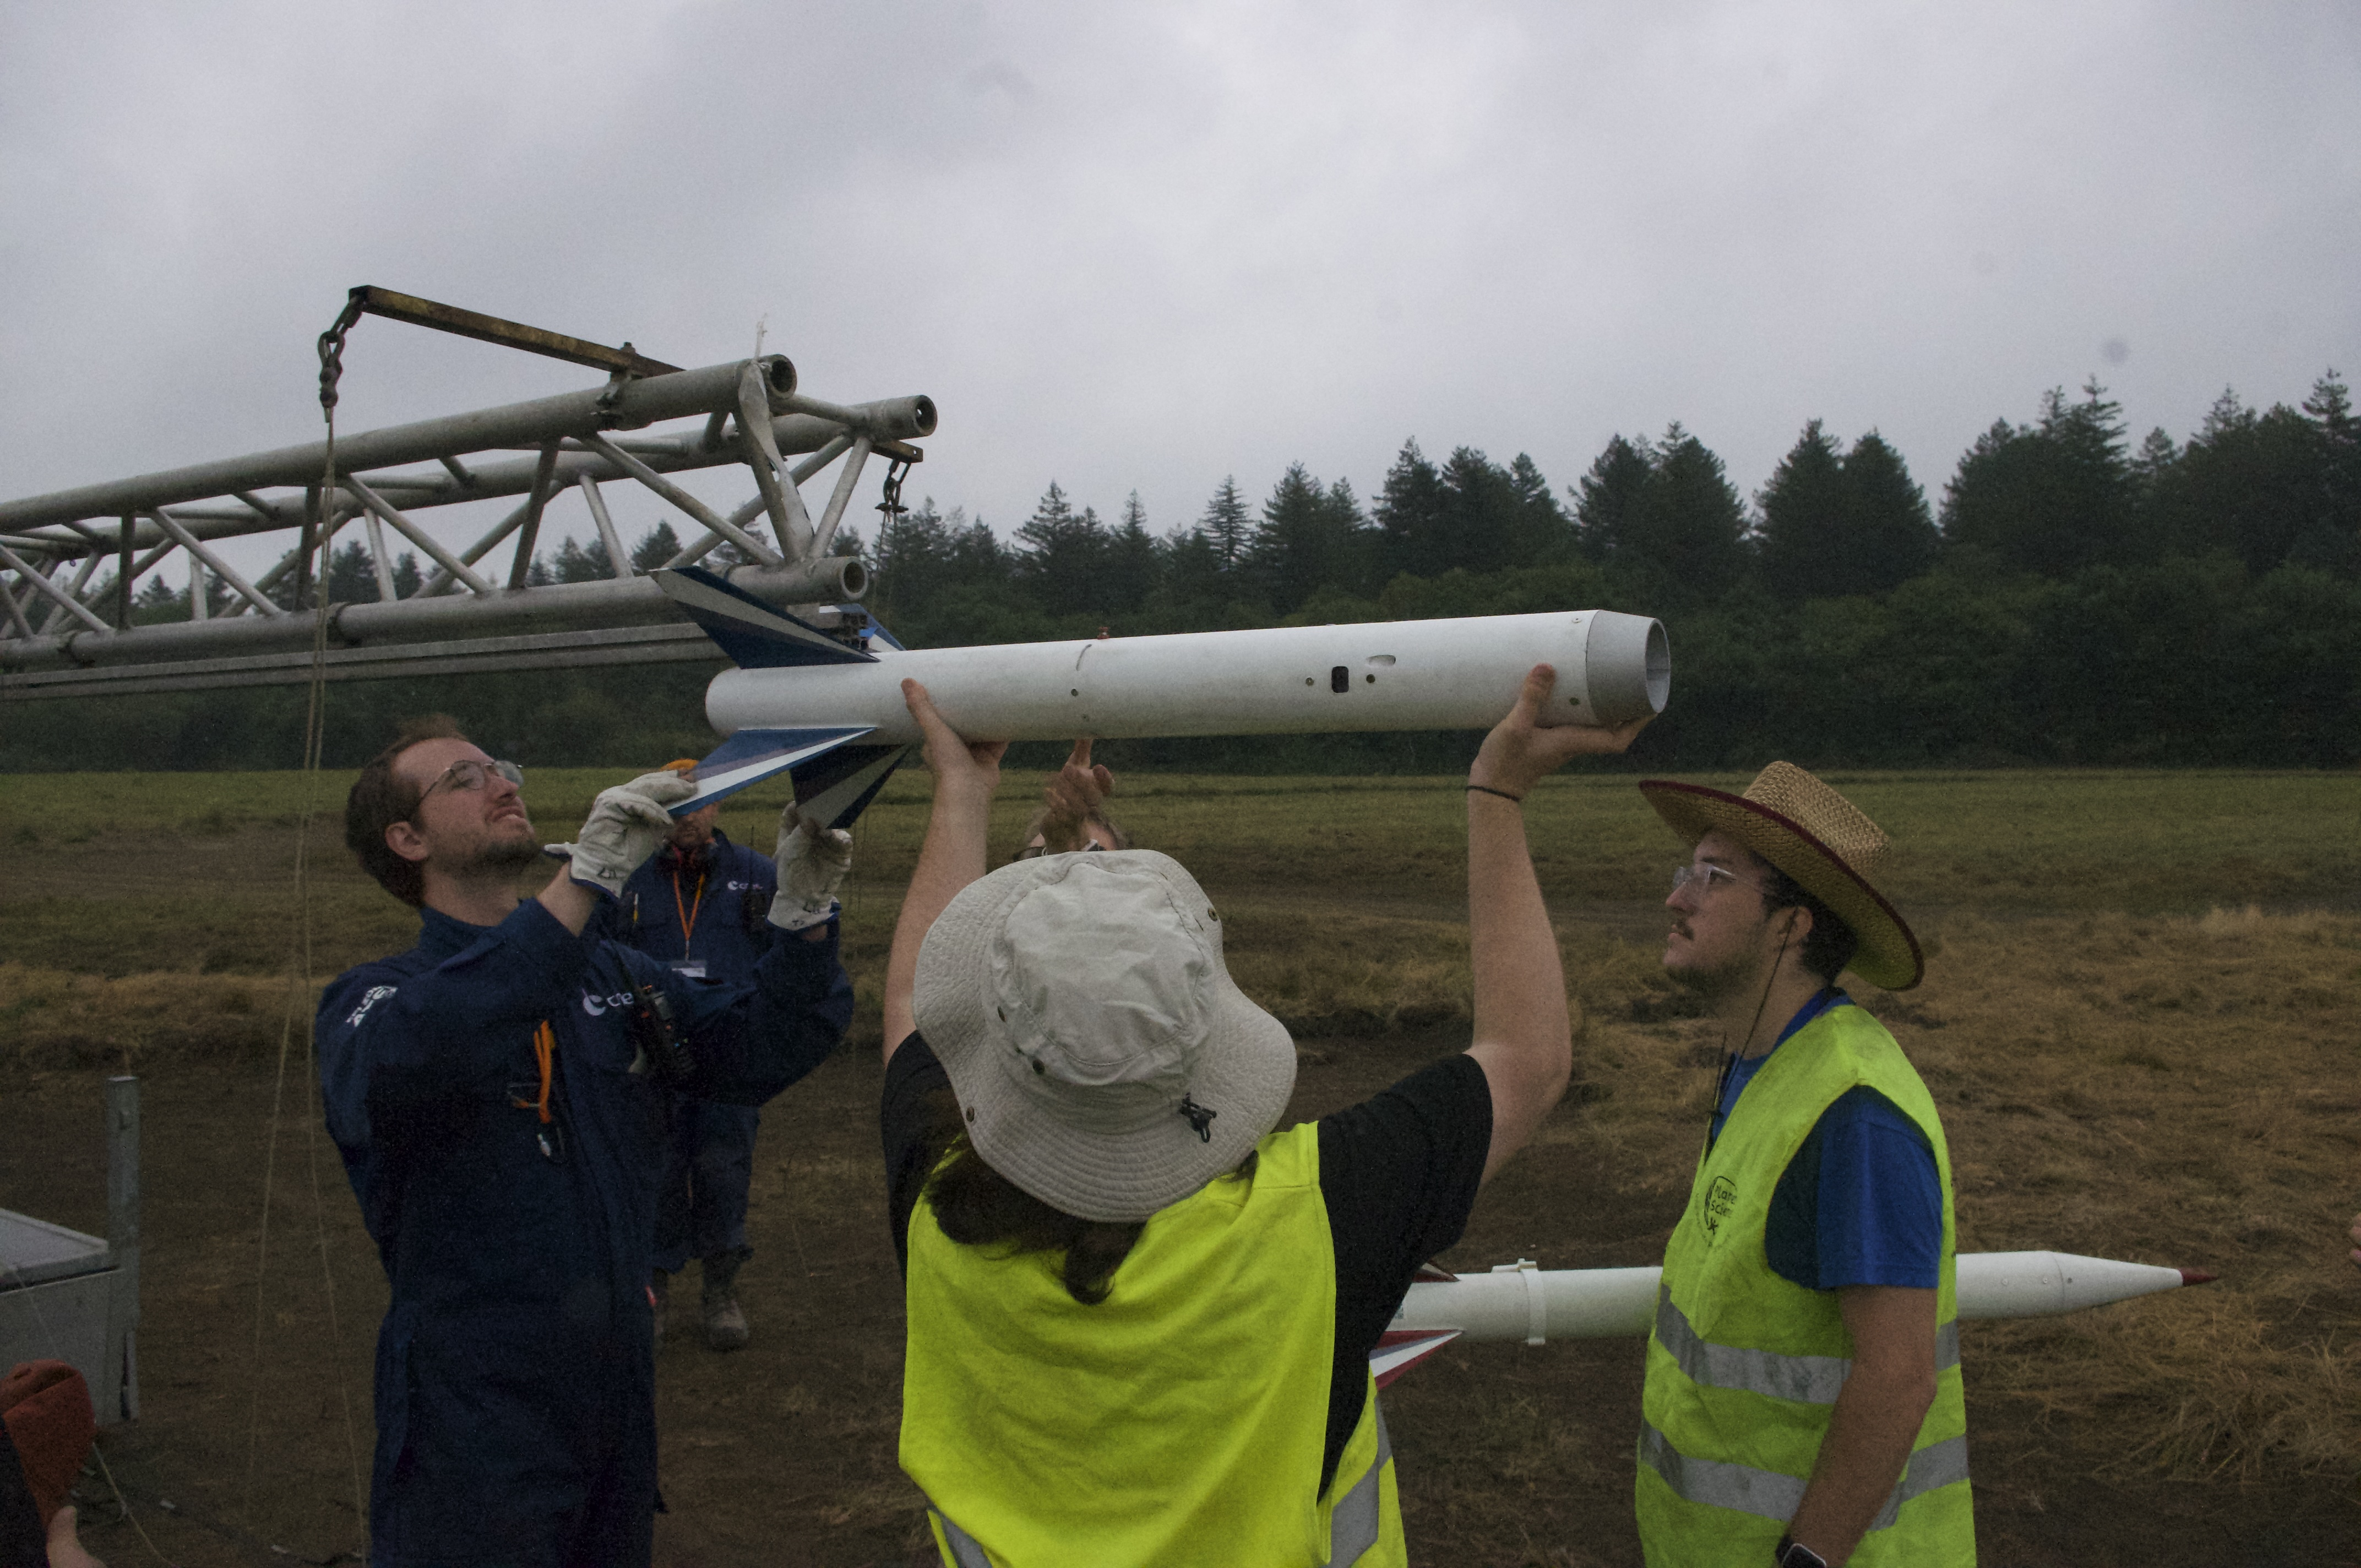
\includegraphics[width=\linewidth]{figures/sp02_lancement17.jpeg}
    \end{subfigure}
    % Deuxième ligne : 2 images
    \begin{subfigure}{0.45\textwidth}
        \centering
        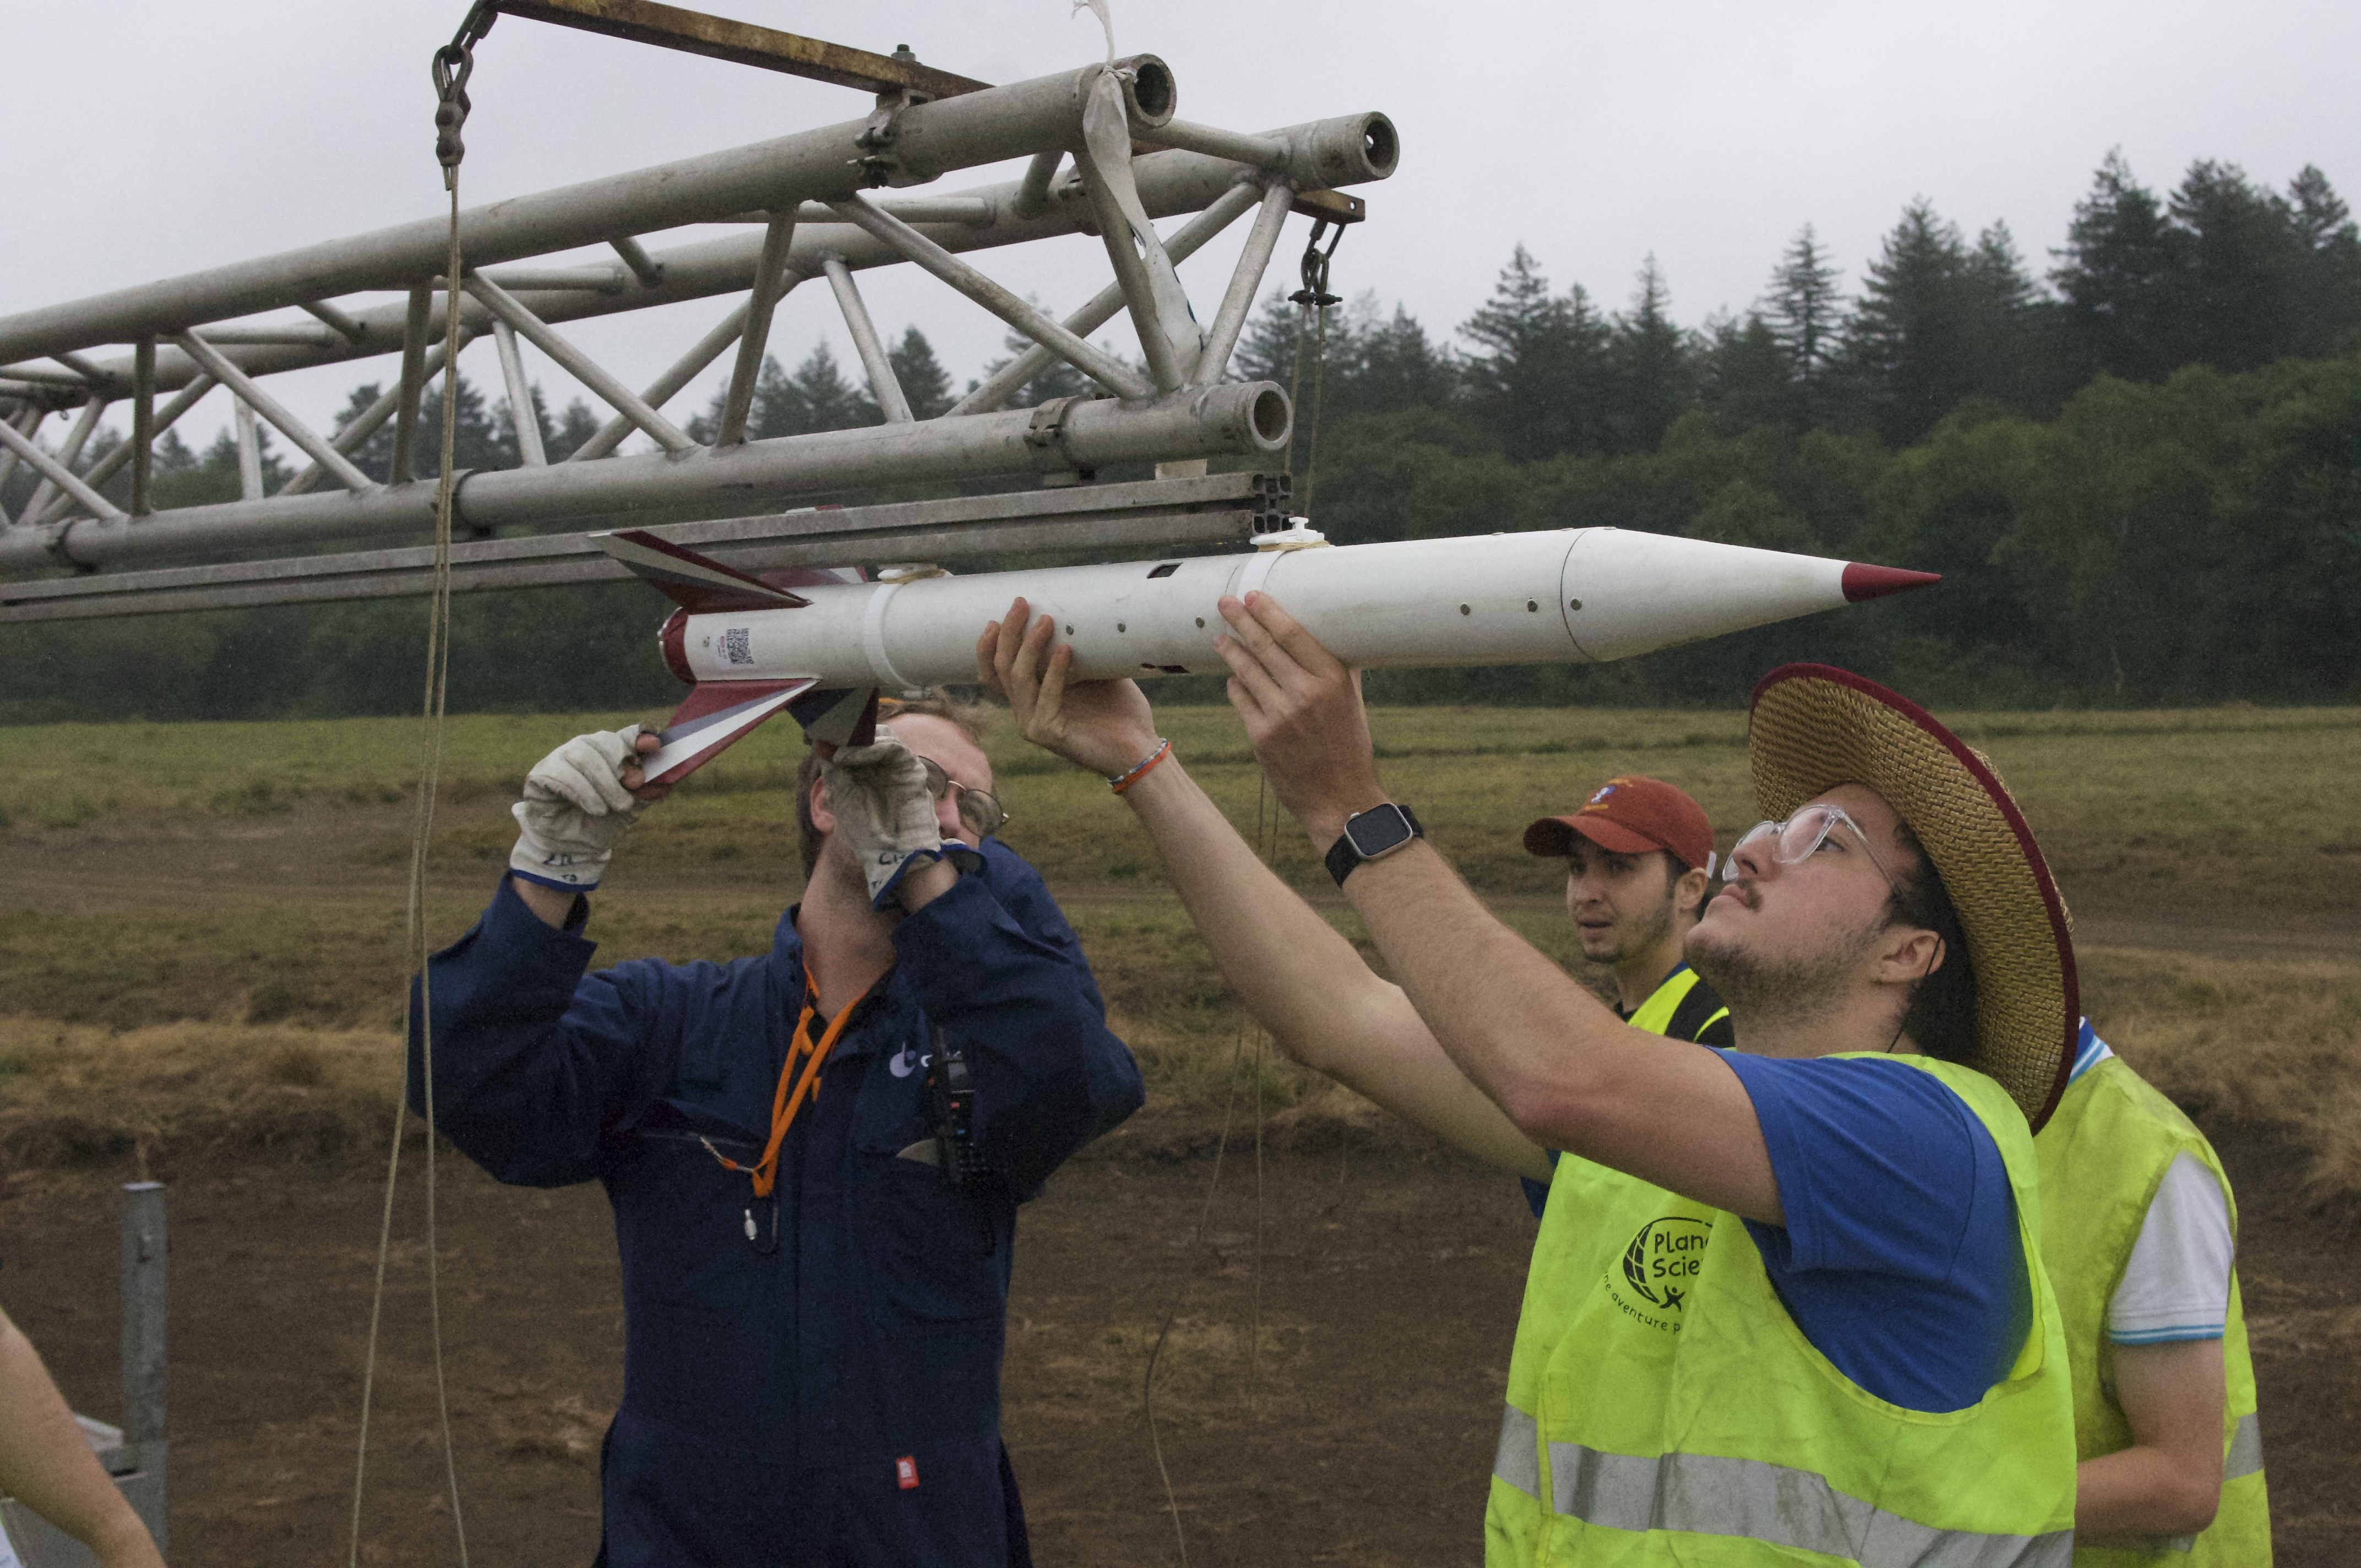
\includegraphics[width=\linewidth]{figures/sp02_lancement20.jpeg}
    \end{subfigure}
    \hfill % Espacement horizontal entre les sous-figures
    \begin{subfigure}{0.45\textwidth}
        \centering
        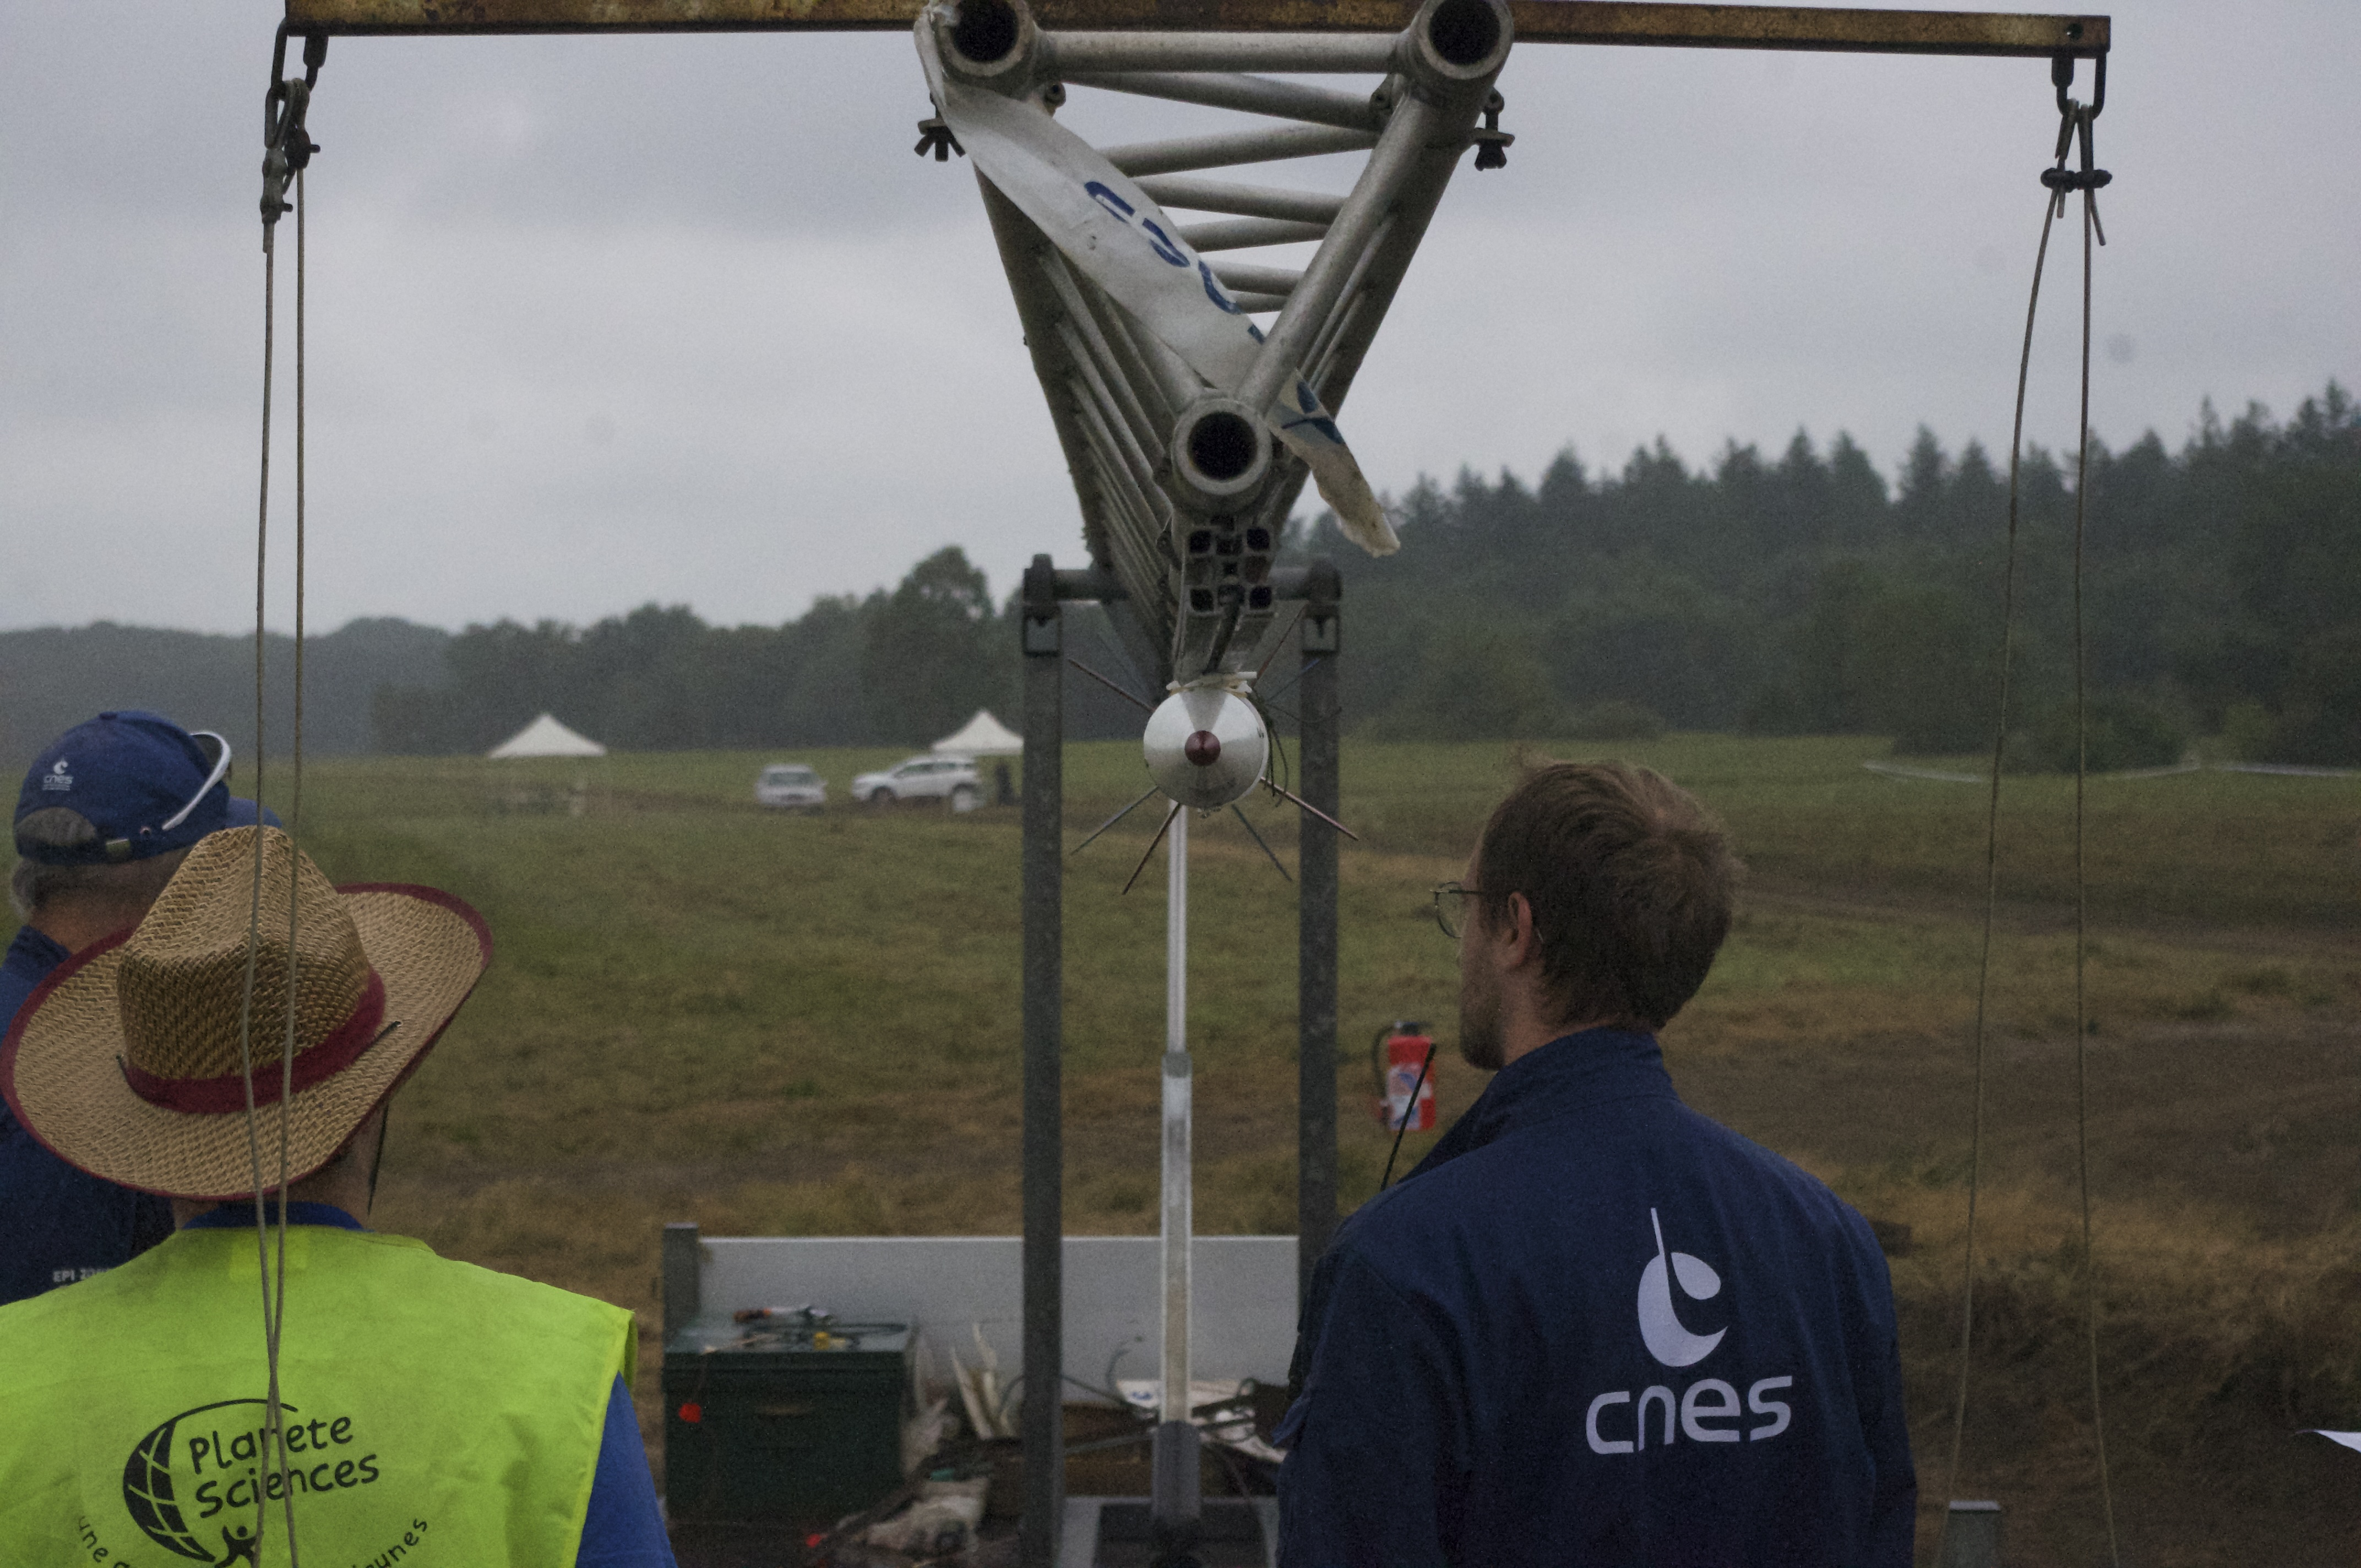
\includegraphics[width=\linewidth]{figures/sp02_lancement21.jpeg}
    \end{subfigure}    
    % Troisième ligne : 2 images
    \begin{subfigure}{0.45\textwidth}
        \centering
        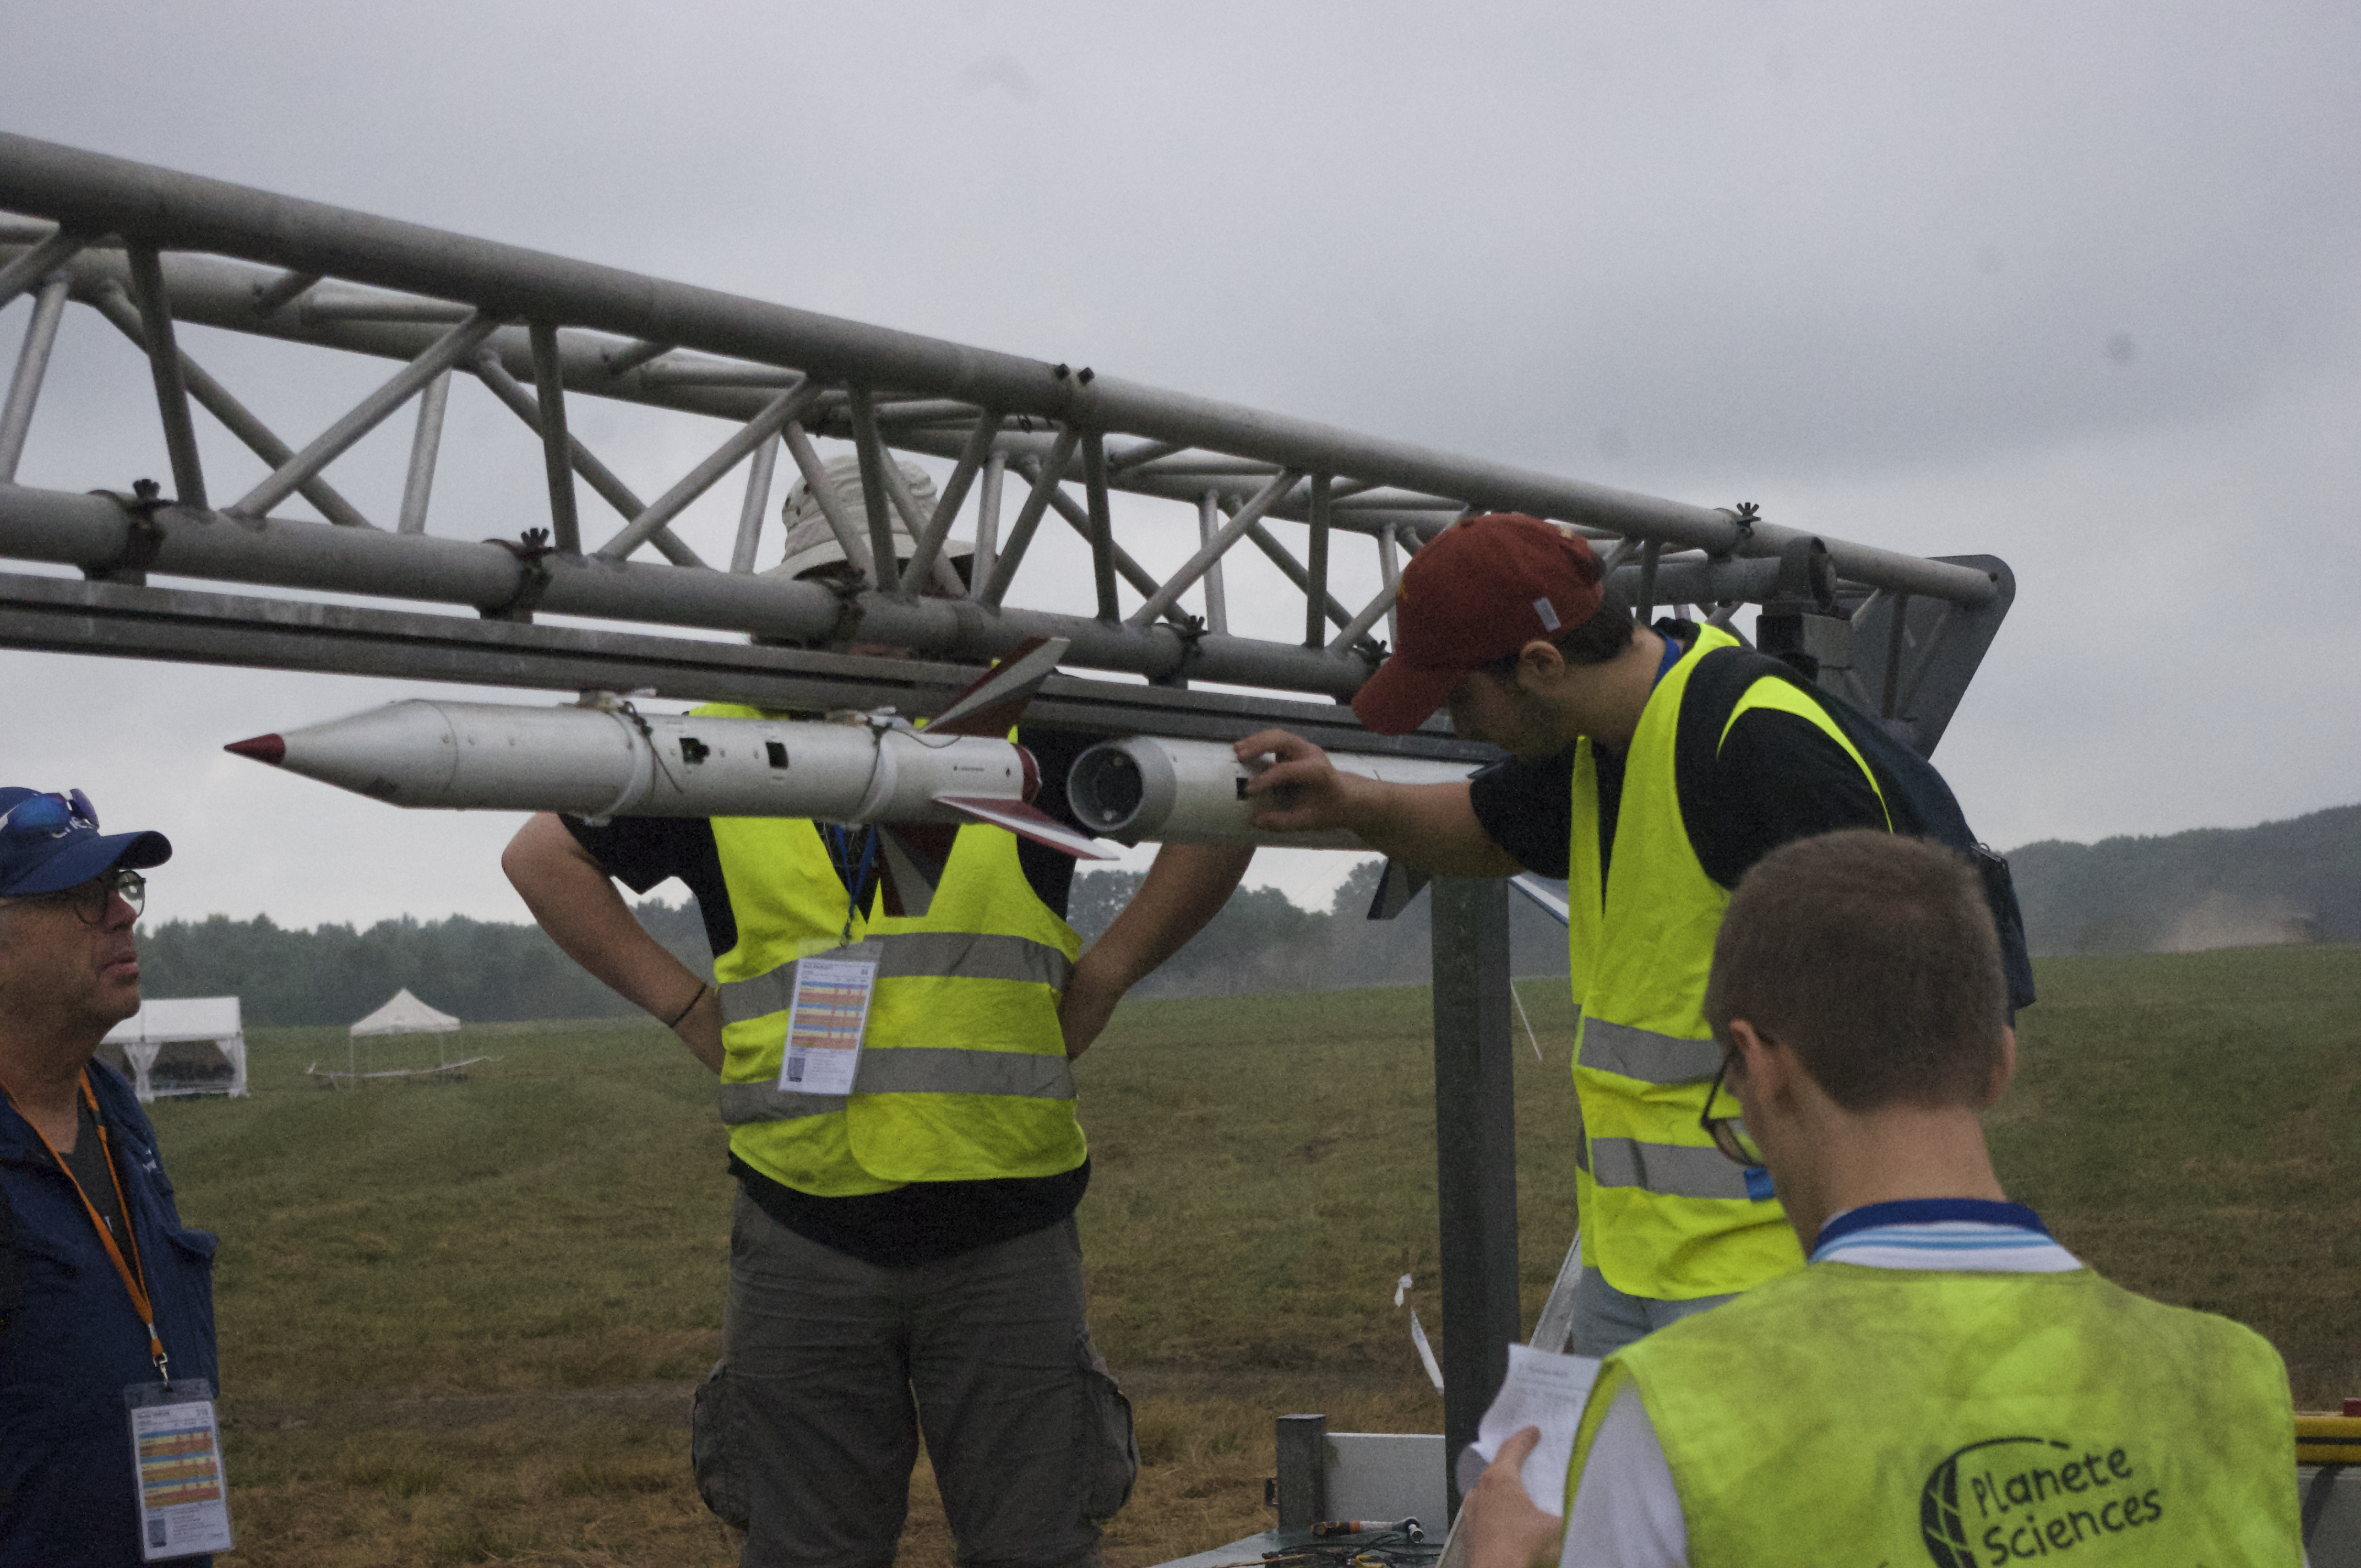
\includegraphics[width=\linewidth]{figures/sp02_lancement24.jpg}
    \end{subfigure}
    \hfill
    \begin{subfigure}{0.45\textwidth}
        \centering
        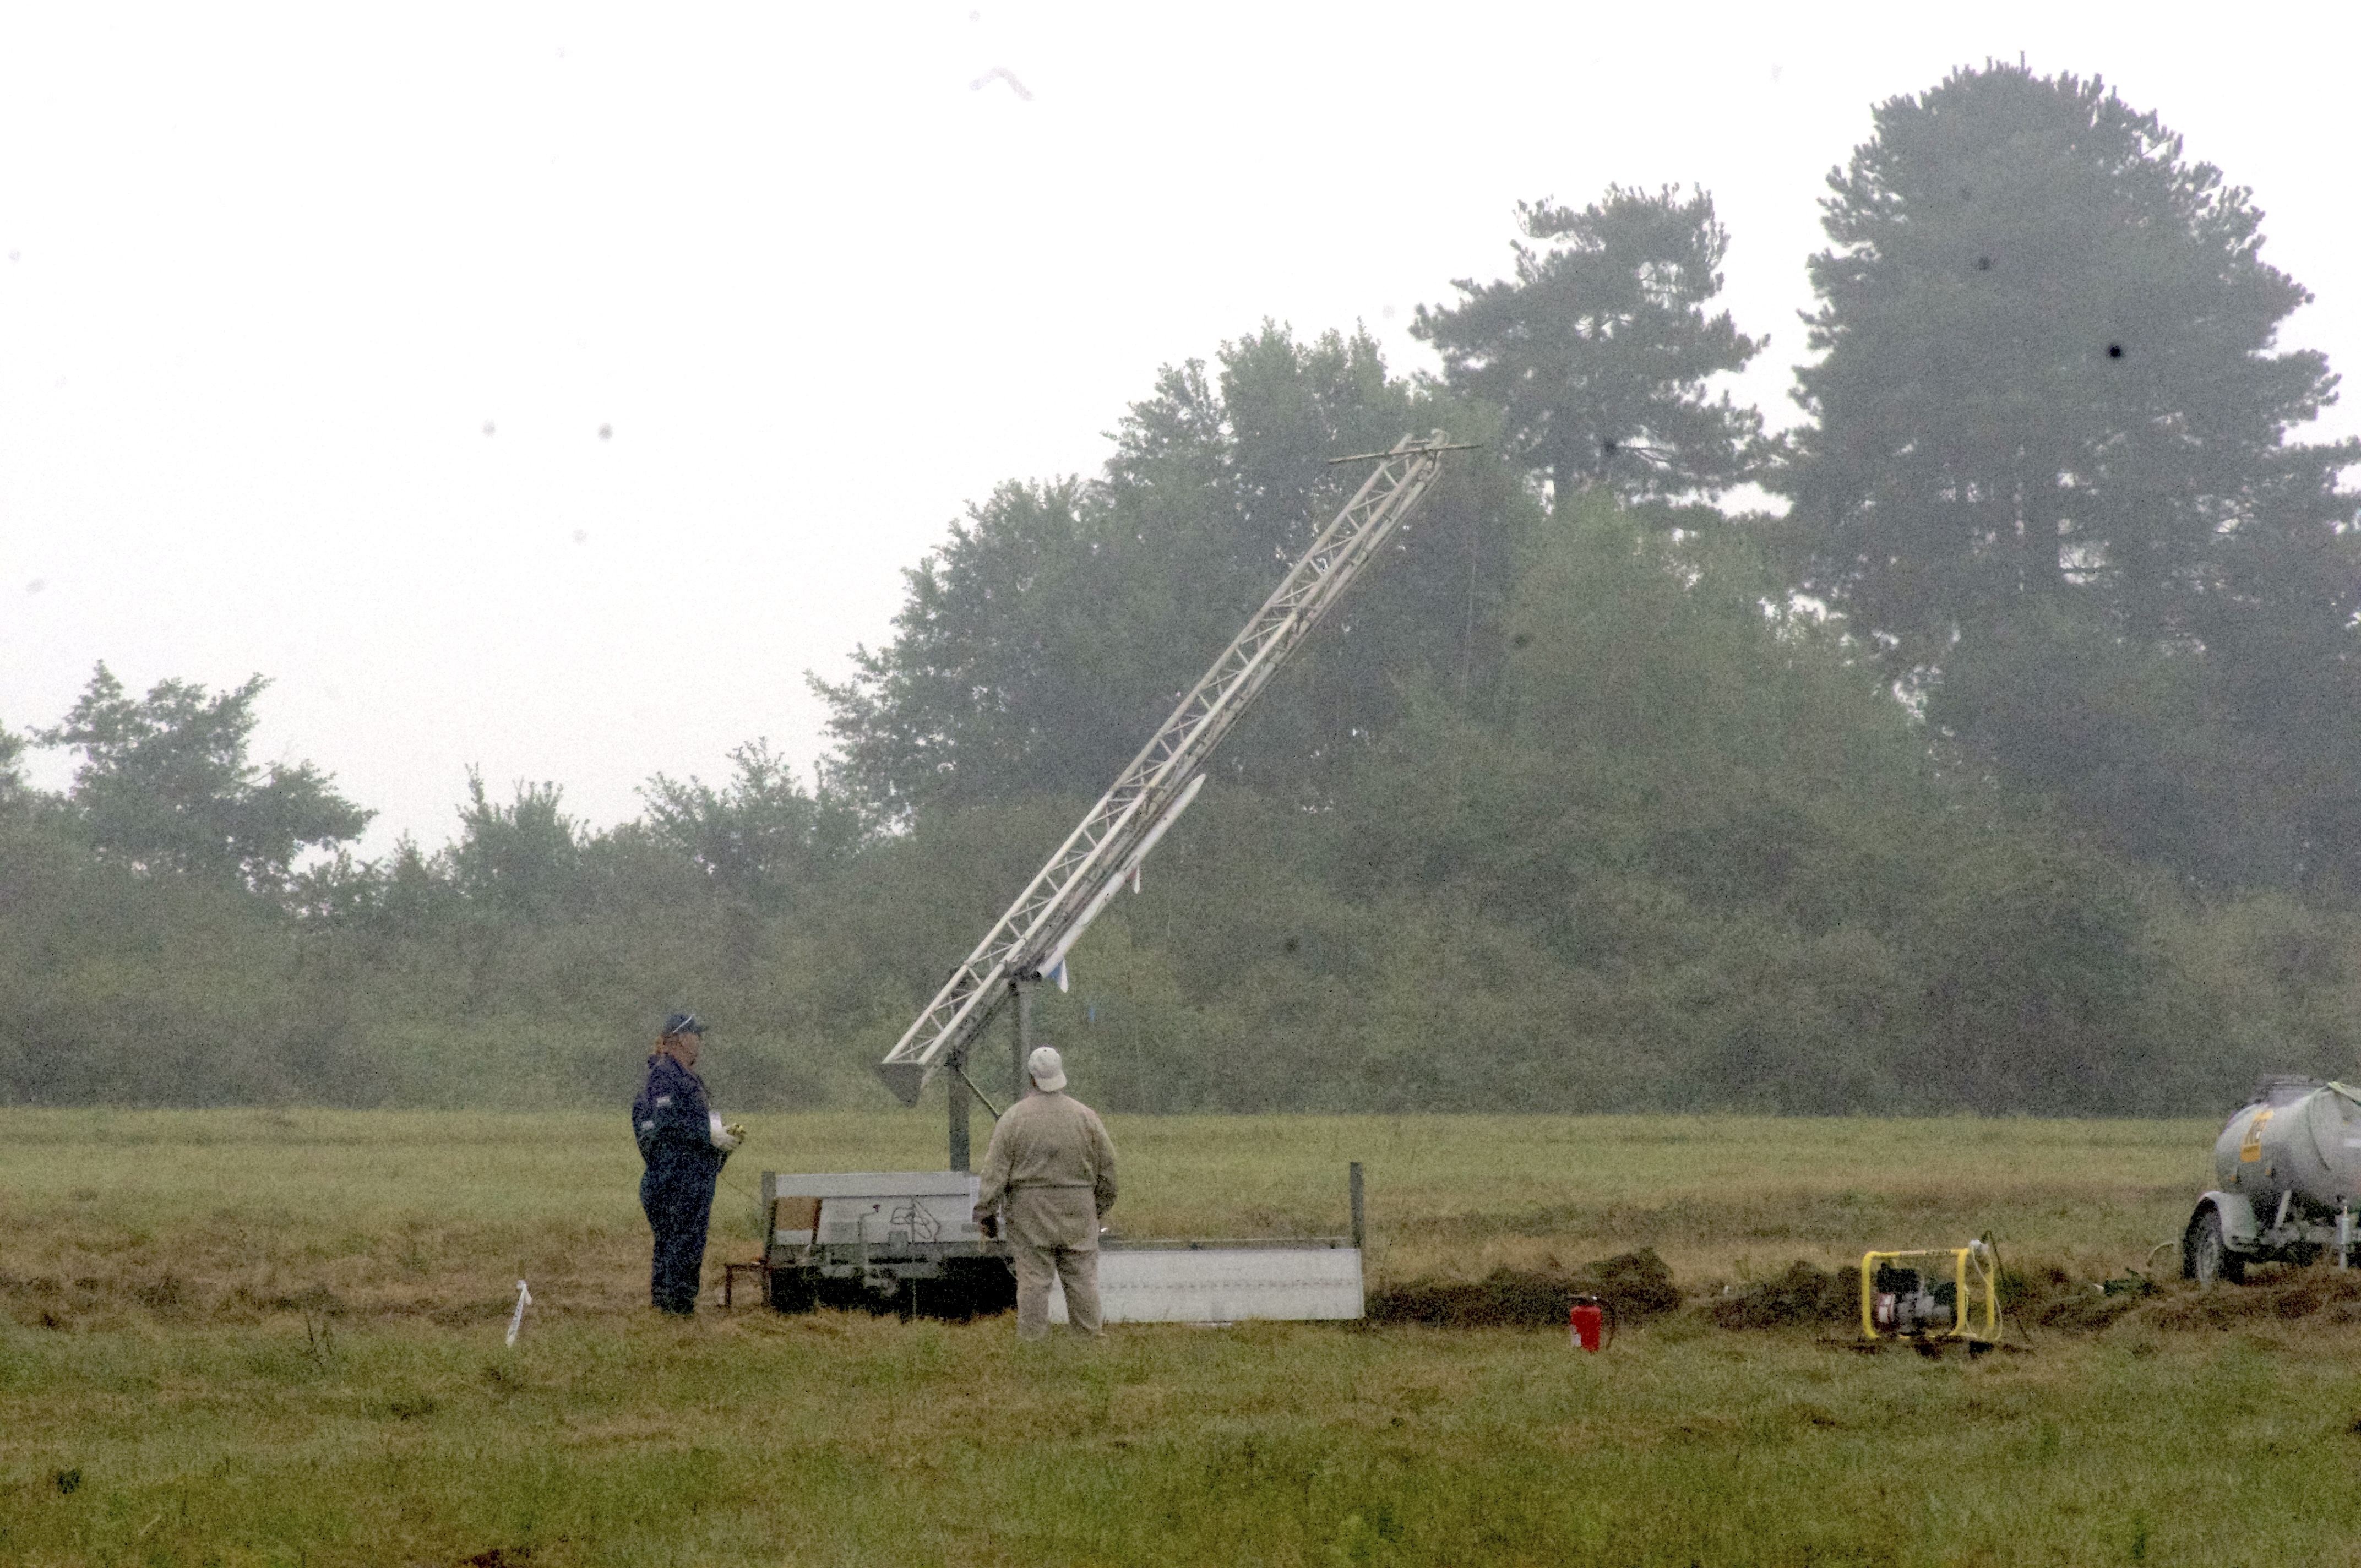
\includegraphics[width=\linewidth]{figures/sp02_lancement29.jpeg}
    \end{subfigure}
    % Légende globale pour les 4 premières images
    \caption{Placement et application des renforts de fibre sur le second étage}
    \label{fig:ailerons_etage2_SP02}
\end{figure}



\newpage
\subsubsection{Recherches et bilan technique}
Les recherches par drones et les rares témoignages ont permis de localiser le deuxième étage, intact en grande partie, 
atterri en zone rouge. Son propulseur ne s'était pas allumé. Après négociations entre le CNES, Planète Sciences et les 
militaires, il a été décidé de récupérer cet étage pour éviter tout danger. Le premier étage, quant à lui, est resté 
introuvable.

\begin{figure}[!ht]
    \centering
    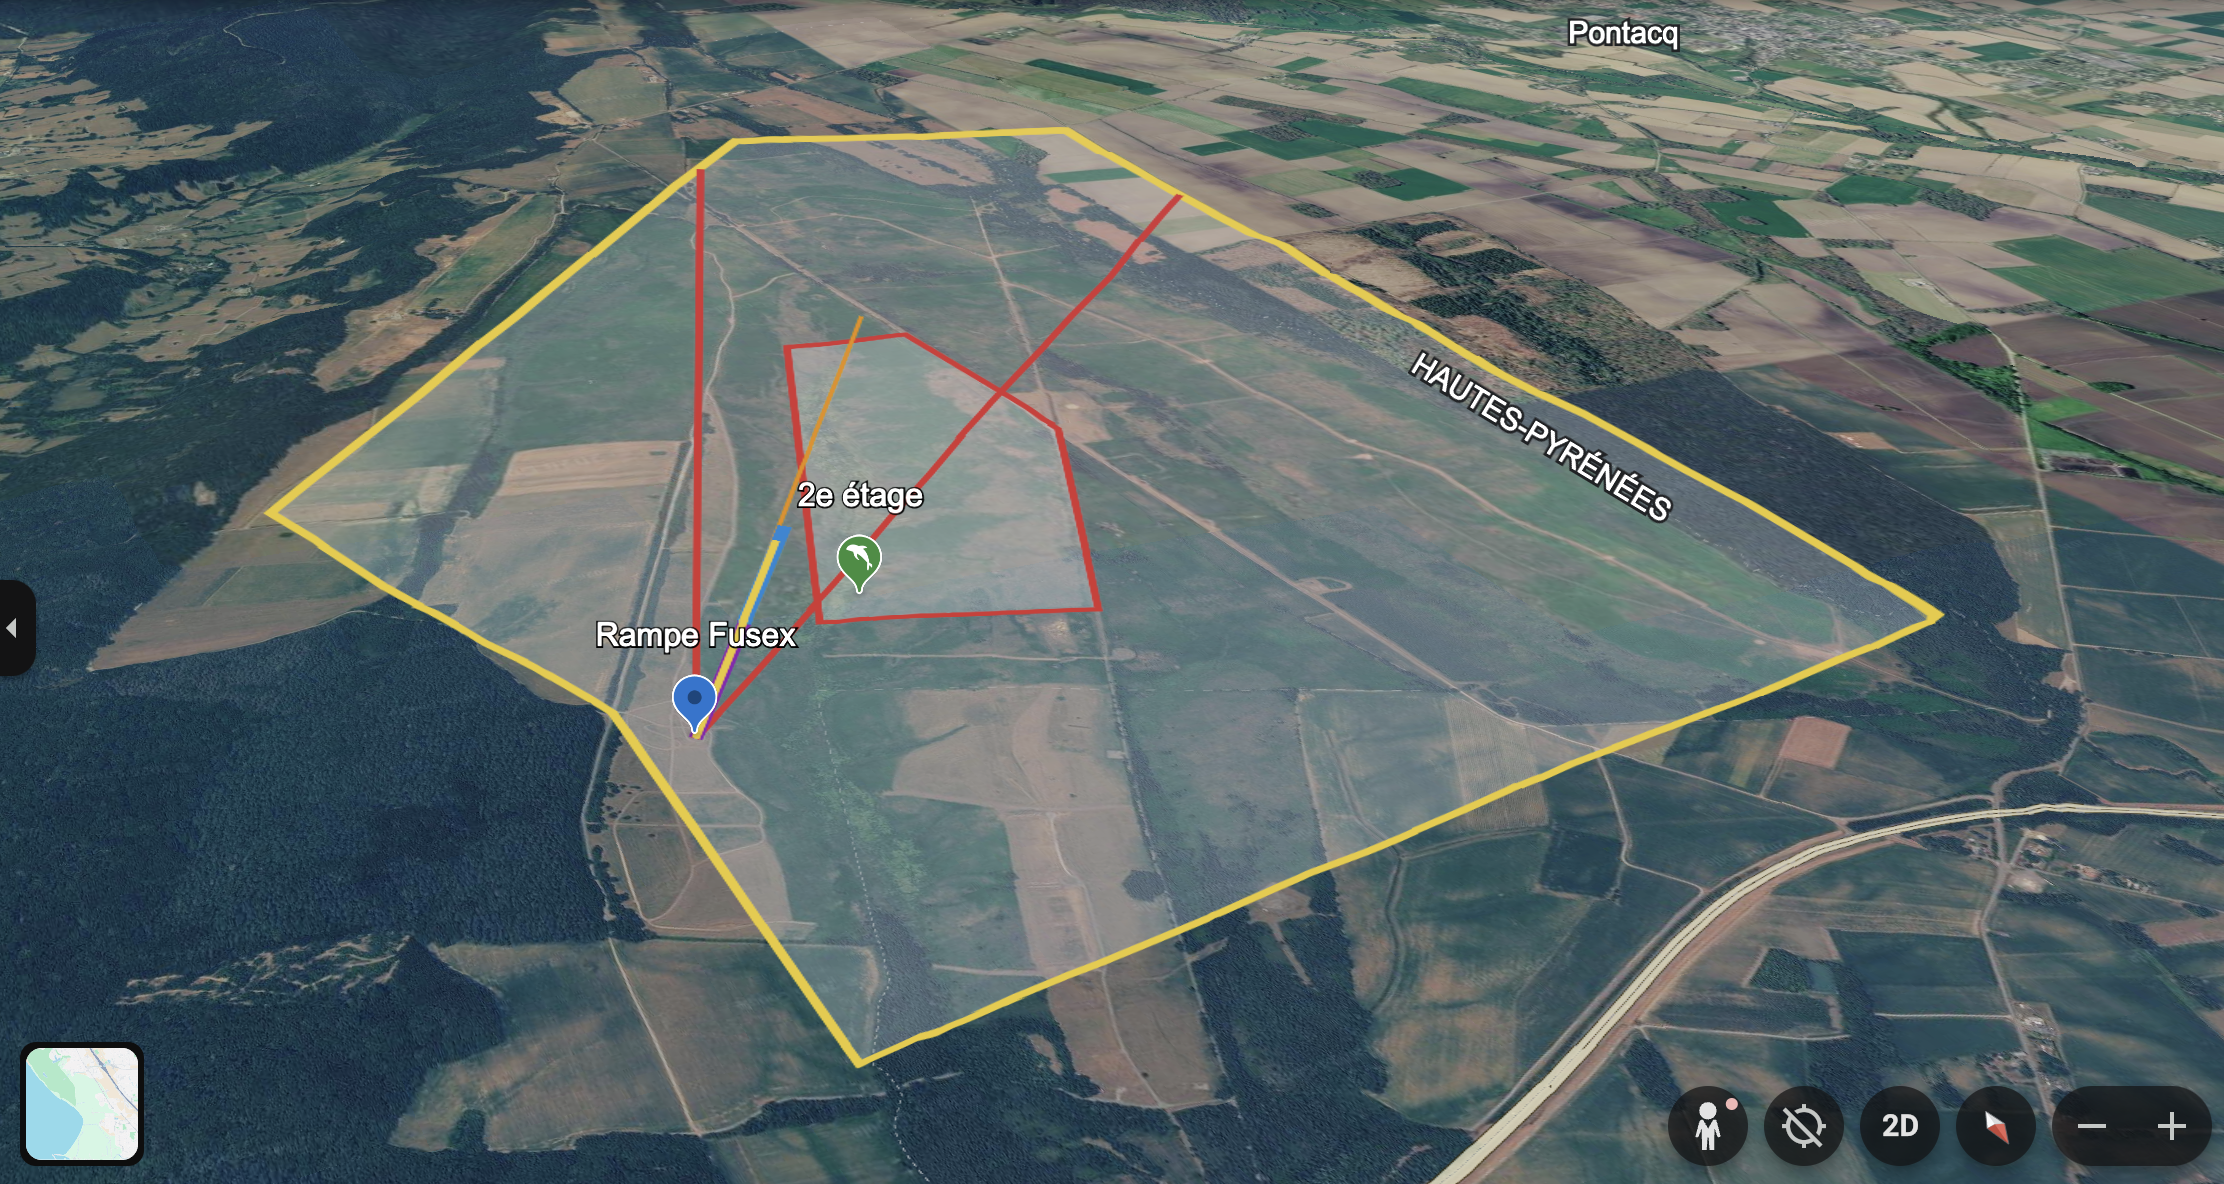
\includegraphics[width=0.58\linewidth]{figures/loc_2nd_etage_SP02.png}
    \caption{Vue satellite des points sur la zone de lancement}
    \label{fig:vue_satellite}
\end{figure}

Le programme de l'expérience, écrit la veille du lancement et jamais testé, contenait des bugs, empêchant la récupération 
de données de vol. Les caméras embarquées n'ont pas fonctionné pour des raisons indéterminées. Les seules informations 
disponibles proviennent des vidéos au sol. \textbf{Néanmoins, l'équipe a réussi à lancer une fusée bi-étage et à effectuer 
une séparation en vol exemplaire.}

\subsubsection{Bilan et perspectives}
Il serait difficile de déterminer précisément ce qui s'est passé ou ce qui aurait pu être fait différemment. Ce projet 
était ambitieux, complexe, et a demandé un investissement considérable de la part de toute l'équipe. Malgré les contraintes 
de temps et de disponibilité, l'équipe a su relever ce défi avec brio.

Ce projet restera comme une expérience inoubliable, marquée par la solidarité, la persévérance et l'innovation. Pour les 
futurs membres de l'AéroIPSA, ce message : \textit{Osez vous lancer dans des projets ambitieux, qui vous dépasseront. 
C'est ainsi que vous grandirez, que vous vivrez des expériences uniques, et que vous réaliserez l'importance d'une équipe 
soudée pour transformer un rêve en réalité.}

\begin{figure}[h!]
    \centering
    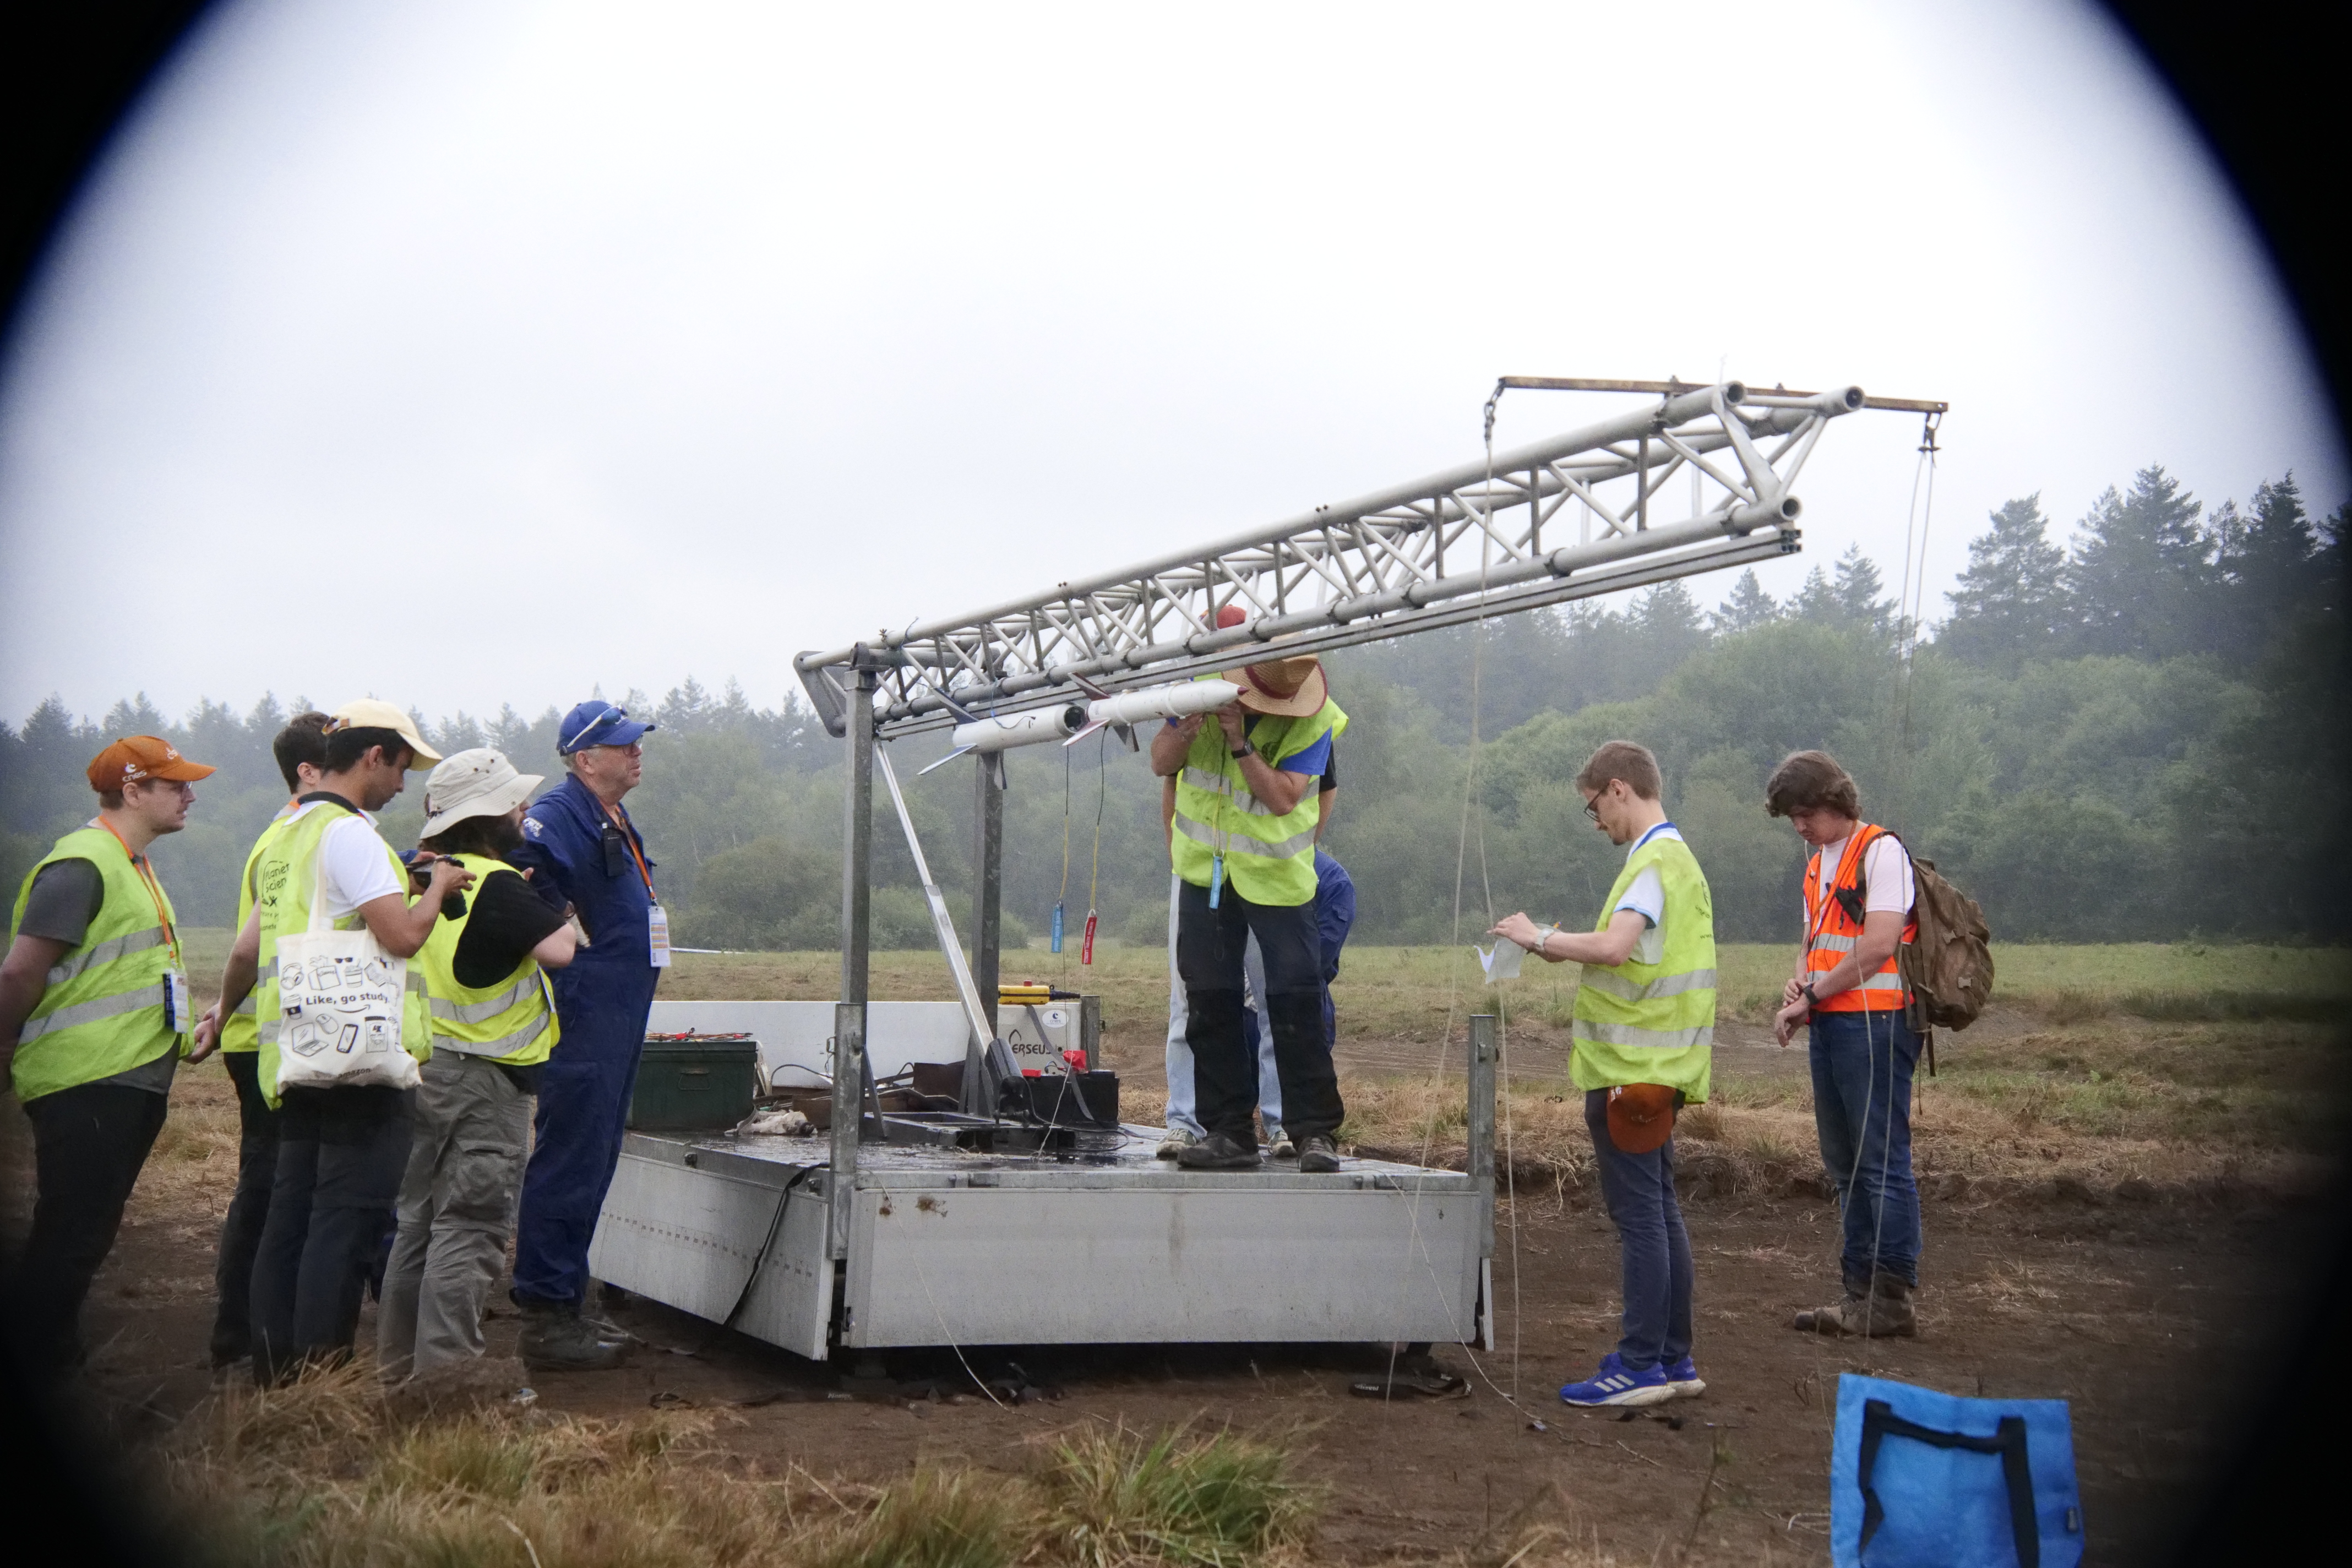
\includegraphics[width=0.8\textwidth]{figures/1057280.jpg}
    \caption{SP-02 en rampe}
    \label{fig:rampe_SP02_oeil}
\end{figure}

\newpage
